% Options for packages loaded elsewhere
\PassOptionsToPackage{unicode}{hyperref}
\PassOptionsToPackage{hyphens}{url}
%
\documentclass[
]{article}
\usepackage{amsmath,amssymb}
\usepackage{lmodern}
\usepackage{iftex}
\ifPDFTeX
  \usepackage[T1]{fontenc}
  \usepackage[utf8]{inputenc}
  \usepackage{textcomp} % provide euro and other symbols
\else % if luatex or xetex
  \usepackage{unicode-math}
  \defaultfontfeatures{Scale=MatchLowercase}
  \defaultfontfeatures[\rmfamily]{Ligatures=TeX,Scale=1}
\fi
% Use upquote if available, for straight quotes in verbatim environments
\IfFileExists{upquote.sty}{\usepackage{upquote}}{}
\IfFileExists{microtype.sty}{% use microtype if available
  \usepackage[]{microtype}
  \UseMicrotypeSet[protrusion]{basicmath} % disable protrusion for tt fonts
}{}
\makeatletter
\@ifundefined{KOMAClassName}{% if non-KOMA class
  \IfFileExists{parskip.sty}{%
    \usepackage{parskip}
  }{% else
    \setlength{\parindent}{0pt}
    \setlength{\parskip}{6pt plus 2pt minus 1pt}}
}{% if KOMA class
  \KOMAoptions{parskip=half}}
\makeatother
\usepackage{xcolor}
\IfFileExists{xurl.sty}{\usepackage{xurl}}{} % add URL line breaks if available
\IfFileExists{bookmark.sty}{\usepackage{bookmark}}{\usepackage{hyperref}}
\hypersetup{
  pdflang={pt-br},
  hidelinks,
  pdfcreator={LaTeX via pandoc}}
\urlstyle{same} % disable monospaced font for URLs
\usepackage[left=0.9cm,right=0.9cm,top=0.7cm,bottom=1.5cm]{geometry}
\usepackage{color}
\usepackage{fancyvrb}
\newcommand{\VerbBar}{|}
\newcommand{\VERB}{\Verb[commandchars=\\\{\}]}
\DefineVerbatimEnvironment{Highlighting}{Verbatim}{commandchars=\\\{\}}
% Add ',fontsize=\small' for more characters per line
\usepackage{framed}
\definecolor{shadecolor}{RGB}{248,248,248}
\newenvironment{Shaded}{\begin{snugshade}}{\end{snugshade}}
\newcommand{\AlertTok}[1]{\textcolor[rgb]{0.94,0.16,0.16}{#1}}
\newcommand{\AnnotationTok}[1]{\textcolor[rgb]{0.56,0.35,0.01}{\textbf{\textit{#1}}}}
\newcommand{\AttributeTok}[1]{\textcolor[rgb]{0.77,0.63,0.00}{#1}}
\newcommand{\BaseNTok}[1]{\textcolor[rgb]{0.00,0.00,0.81}{#1}}
\newcommand{\BuiltInTok}[1]{#1}
\newcommand{\CharTok}[1]{\textcolor[rgb]{0.31,0.60,0.02}{#1}}
\newcommand{\CommentTok}[1]{\textcolor[rgb]{0.56,0.35,0.01}{\textit{#1}}}
\newcommand{\CommentVarTok}[1]{\textcolor[rgb]{0.56,0.35,0.01}{\textbf{\textit{#1}}}}
\newcommand{\ConstantTok}[1]{\textcolor[rgb]{0.00,0.00,0.00}{#1}}
\newcommand{\ControlFlowTok}[1]{\textcolor[rgb]{0.13,0.29,0.53}{\textbf{#1}}}
\newcommand{\DataTypeTok}[1]{\textcolor[rgb]{0.13,0.29,0.53}{#1}}
\newcommand{\DecValTok}[1]{\textcolor[rgb]{0.00,0.00,0.81}{#1}}
\newcommand{\DocumentationTok}[1]{\textcolor[rgb]{0.56,0.35,0.01}{\textbf{\textit{#1}}}}
\newcommand{\ErrorTok}[1]{\textcolor[rgb]{0.64,0.00,0.00}{\textbf{#1}}}
\newcommand{\ExtensionTok}[1]{#1}
\newcommand{\FloatTok}[1]{\textcolor[rgb]{0.00,0.00,0.81}{#1}}
\newcommand{\FunctionTok}[1]{\textcolor[rgb]{0.00,0.00,0.00}{#1}}
\newcommand{\ImportTok}[1]{#1}
\newcommand{\InformationTok}[1]{\textcolor[rgb]{0.56,0.35,0.01}{\textbf{\textit{#1}}}}
\newcommand{\KeywordTok}[1]{\textcolor[rgb]{0.13,0.29,0.53}{\textbf{#1}}}
\newcommand{\NormalTok}[1]{#1}
\newcommand{\OperatorTok}[1]{\textcolor[rgb]{0.81,0.36,0.00}{\textbf{#1}}}
\newcommand{\OtherTok}[1]{\textcolor[rgb]{0.56,0.35,0.01}{#1}}
\newcommand{\PreprocessorTok}[1]{\textcolor[rgb]{0.56,0.35,0.01}{\textit{#1}}}
\newcommand{\RegionMarkerTok}[1]{#1}
\newcommand{\SpecialCharTok}[1]{\textcolor[rgb]{0.00,0.00,0.00}{#1}}
\newcommand{\SpecialStringTok}[1]{\textcolor[rgb]{0.31,0.60,0.02}{#1}}
\newcommand{\StringTok}[1]{\textcolor[rgb]{0.31,0.60,0.02}{#1}}
\newcommand{\VariableTok}[1]{\textcolor[rgb]{0.00,0.00,0.00}{#1}}
\newcommand{\VerbatimStringTok}[1]{\textcolor[rgb]{0.31,0.60,0.02}{#1}}
\newcommand{\WarningTok}[1]{\textcolor[rgb]{0.56,0.35,0.01}{\textbf{\textit{#1}}}}
\usepackage{longtable,booktabs,array}
\usepackage{calc} % for calculating minipage widths
% Correct order of tables after \paragraph or \subparagraph
\usepackage{etoolbox}
\makeatletter
\patchcmd\longtable{\par}{\if@noskipsec\mbox{}\fi\par}{}{}
\makeatother
% Allow footnotes in longtable head/foot
\IfFileExists{footnotehyper.sty}{\usepackage{footnotehyper}}{\usepackage{footnote}}
\makesavenoteenv{longtable}
\usepackage{graphicx}
\makeatletter
\def\maxwidth{\ifdim\Gin@nat@width>\linewidth\linewidth\else\Gin@nat@width\fi}
\def\maxheight{\ifdim\Gin@nat@height>\textheight\textheight\else\Gin@nat@height\fi}
\makeatother
% Scale images if necessary, so that they will not overflow the page
% margins by default, and it is still possible to overwrite the defaults
% using explicit options in \includegraphics[width, height, ...]{}
\setkeys{Gin}{width=\maxwidth,height=\maxheight,keepaspectratio}
% Set default figure placement to htbp
\makeatletter
\def\fps@figure{htbp}
\makeatother
\setlength{\emergencystretch}{3em} % prevent overfull lines
\providecommand{\tightlist}{%
  \setlength{\itemsep}{0pt}\setlength{\parskip}{0pt}}
\setcounter{secnumdepth}{-\maxdimen} % remove section numbering
\ifLuaTeX
\usepackage[bidi=basic]{babel}
\else
\usepackage[bidi=default]{babel}
\fi
\babelprovide[main,import]{brazilian}
% get rid of language-specific shorthands (see #6817):
\let\LanguageShortHands\languageshorthands
\def\languageshorthands#1{}
\usepackage{fancyhdr}
\ifLuaTeX
  \usepackage{selnolig}  % disable illegal ligatures
\fi

\title{Geração de relatórios e apresentações com R}
\usepackage{etoolbox}
\makeatletter
\providecommand{\subtitle}[1]{% add subtitle to \maketitle
  \apptocmd{\@title}{\par {\large #1 \par}}{}{}
}
\makeatother
\subtitle{Aplicação prática no contexto de ocorrências aeronáuticas}
\author{João Matheus Slujala Krüger Taborda Hneda}
\date{19/06/2022}

\begin{document}
\maketitle

\renewcommand*\contentsname{Sumário}
{
\setcounter{tocdepth}{5}
\tableofcontents
}
\newpage

\hypertarget{introduuxe7uxe3o}{%
\section{Introdução}\label{introduuxe7uxe3o}}

Quando o assunto é aviação civil e transporte aéreo, vários eventos ou
intercorrências podem ocorrer pelo percurso. Formalmente falando, esses
eventos podem ser chamados de ocorrências aeronáuticas.

Ocorrência aeronáutica é qualquer evento envolvendo aeronave que poderá
ser classificado como incidente, incidente grave ou acidente
\href{https://www3.fmb.unesp.br/sete/pluginfile.php/20354/mod_page/content/2/A_Investigacao_de_acidentes_aeronauticos_Conforme_a_Lei_no_7.pdf}{(link)},
permitindo ao SIPAER (Sistema de Investigação e Prevenção de Acidentes
Aeronáuticos) a adoção dos procedimentos pertinentes.

\begin{itemize}
\tightlist
\item
  Incidente é toda ocorrência aeronáutica que não chega a se
  caracterizar como um acidente mas que afeta ou possa afetar a
  segurança da operação.
\item
  Incidente grave é um incidente que ocorre sob circunstâncias em que um
  acidente quase ocorreu.
\item
  Acidente é uma ocorrência tal que qualquer pessoa sofra lesão grave ou
  morra.
\end{itemize}

Dadas essas possíveis classificações de uma ocorrência aeronáutica, é
importante conhecer fatores que estão associados a ocorrências
aeronáuticas perigosas com objetivos de prevenção.

\begin{figure}

{\centering 
\includegraphics[width=400px]{imagens/brasao_fab} 

}

\caption{Gládio - Símbolo  da Força Aérea Brasileira}\label{fig:unnamed-chunk-1}
\end{figure}

\newpage

\hypertarget{apresentauxe7uxe3o-do-problema}{%
\section{Apresentação do
problema}\label{apresentauxe7uxe3o-do-problema}}

\begin{itemize}
\item
  O trabalho consiste em gerar documentos (relatórios e apresentação)
  resultantes da exploração da base de dados ``Ocorrências Aeronáuticas
  na Aviação Civil Brasileira''
\item
  A base de dados é composta por 5 tabelas que são gerenciadas pelo
  Centro de Investigação e Prevenção de Acidentes Aeronáuticos (CENIPA)
  - Organização Militar Brasileira vinculada ao Comando da Aeronáutica
\item
  Para obter as tabelas, consulte o link:
  \url{https://dados.gov.br/dataset/ocorrencias-aeronauticas-da-aviacao-civil-brasileira}
\item
  As tabelas têm informações sobre: aeronaves envolvidas, fatalidades,
  local, data, tipo de ocorrência, fatores contribuintes, etc.
\end{itemize}

\begin{figure}

{\centering 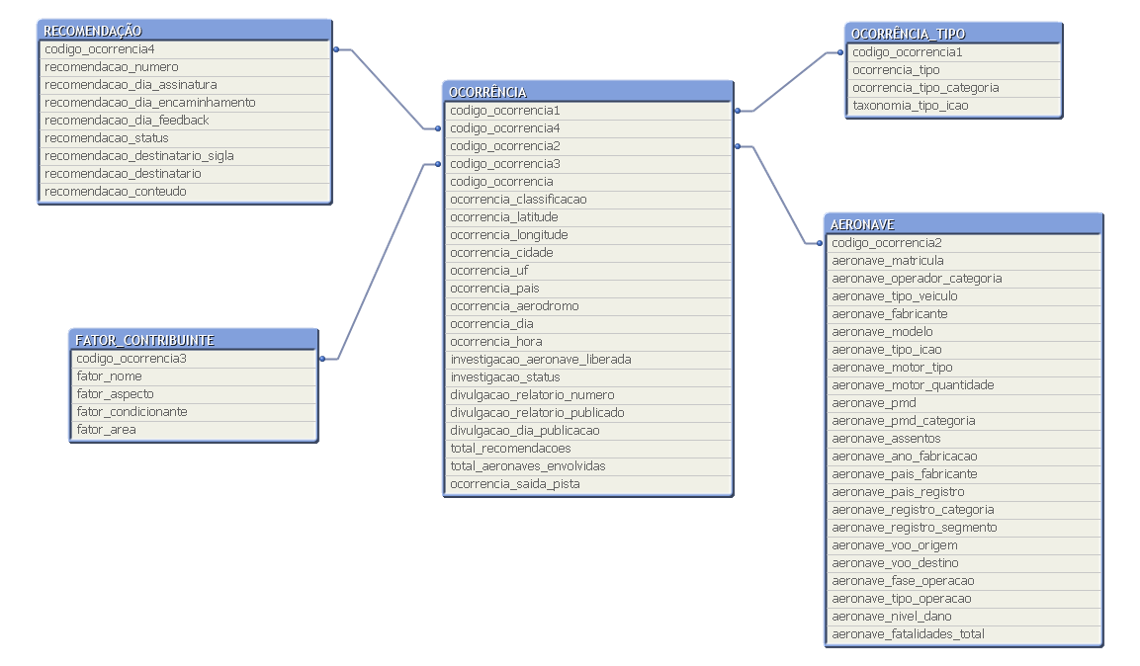
\includegraphics[width=550px]{imagens/modelo_dados} 

}

\caption{Tabelas das ocorrências aeronáuticas}\label{fig:unnamed-chunk-2}
\end{figure}

O nome das tabelas são: OCORRÊNCIA, OCORRÊNCIA\_TIPO, AERONAVE,
FATOR\_CONTRIBUINTE E RECOMENDAÇÃO. Para a realização desse teste,
deu-se ênfase às tabelas OCORRÊNCIA e OCORRÊNCIA\_TIPO.

\newpage

\hypertarget{explicauxe7uxe3o-do-processo-utilizado}{%
\section{Explicação do processo
utilizado}\label{explicauxe7uxe3o-do-processo-utilizado}}

\hypertarget{download-das-tabelas-em-.csv}{%
\subsection{Download das tabelas em
.csv}\label{download-das-tabelas-em-.csv}}

\begin{figure}

{\centering 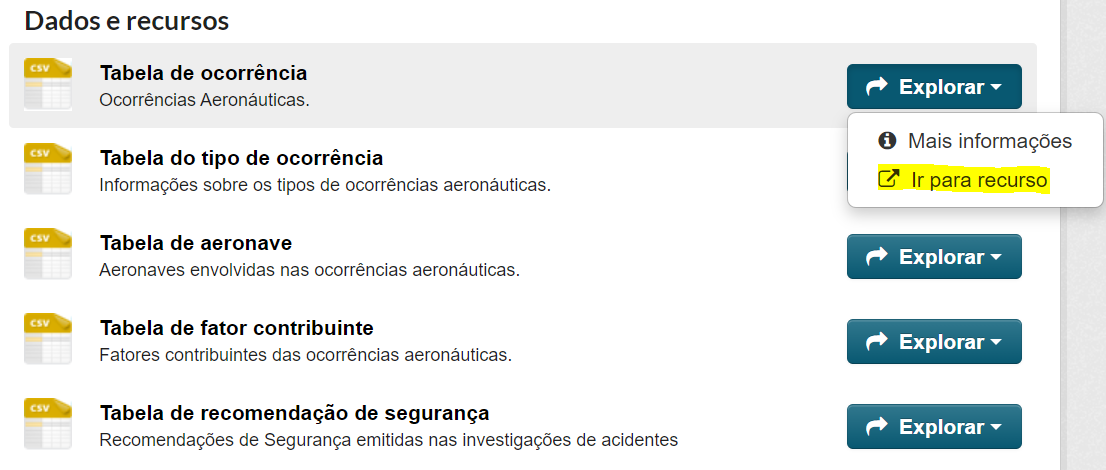
\includegraphics[width=450px]{imagens/dados_e_recursos} 

}

\caption{Link: https://dados.gov.br/dataset/ocorrencias-aeronauticas-da-aviacao-civil-brasileira}\label{fig:unnamed-chunk-3}
\end{figure}

\hypertarget{fluxo-de-trabalho-com-pacotes-da-linguagem-r}{%
\subsection{Fluxo de trabalho com pacotes da linguagem
R}\label{fluxo-de-trabalho-com-pacotes-da-linguagem-r}}

\begin{figure}

{\centering 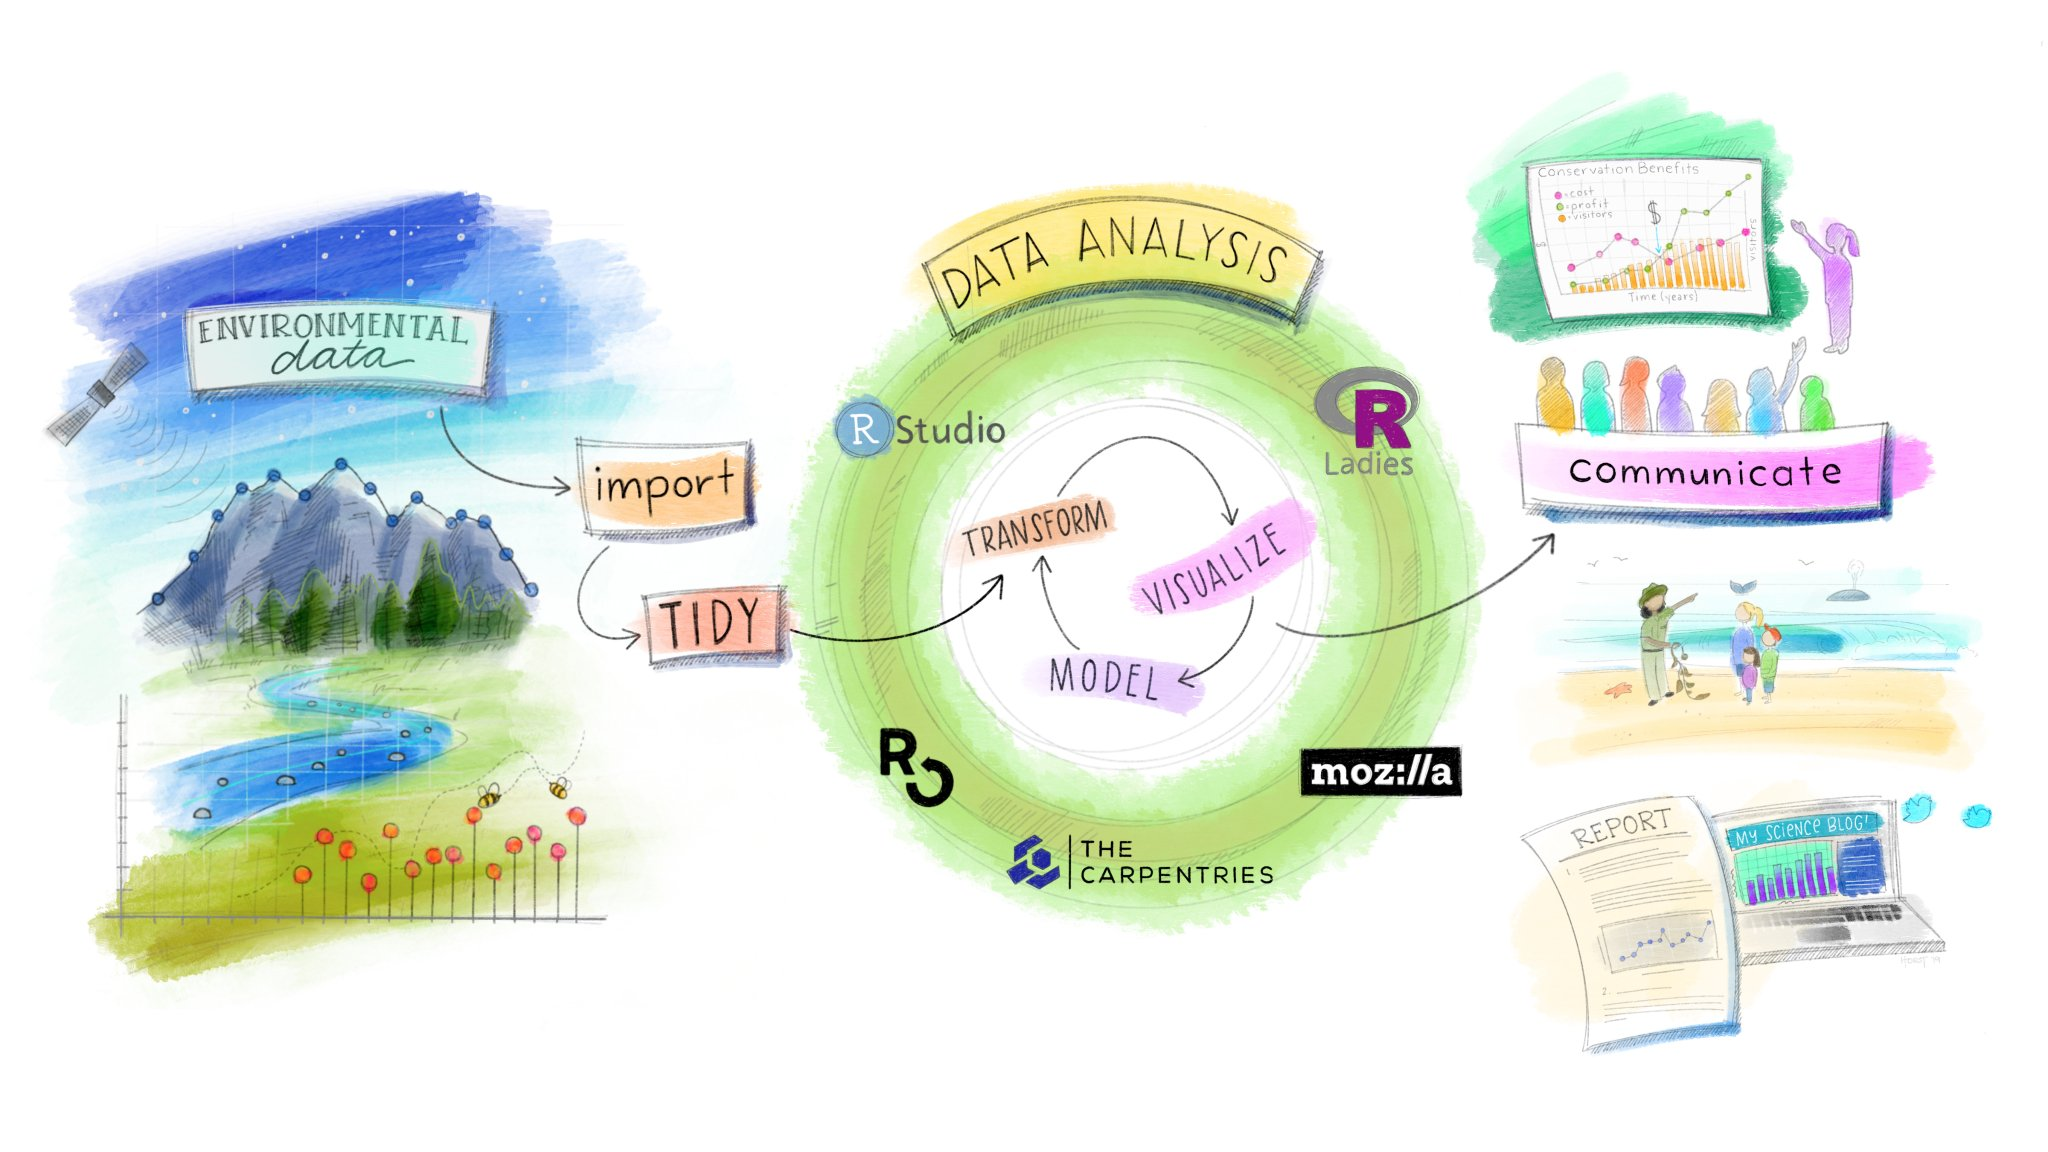
\includegraphics[width=0.55\linewidth]{imagens/ciclo_ciencia_dados} 

}

\caption{Fluxo de trabalho em Estatística e Ciência de Dados}\label{fig:unnamed-chunk-4}
\end{figure}

\begin{figure}

{\centering 
\includegraphics[width=0.1\linewidth]{imagens/dplyr} 
\includegraphics[width=0.1\linewidth]{imagens/DBI} 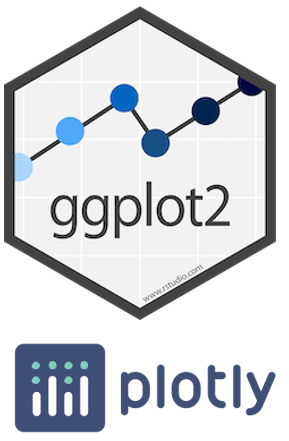
\includegraphics[width=0.1\linewidth]{imagens/ggplot2_plotly} 
\includegraphics[width=0.1\linewidth]{imagens/highcharter} 
\includegraphics[width=0.1\linewidth]{imagens/hex-rmarkdown} 
\includegraphics[width=0.1\linewidth]{imagens/xaringan} 

}

\caption{Alguns pacotes da linguagem R}\label{fig:unnamed-chunk-5}
\end{figure}

Os dados foram obtidos das tabelas baixadas por meio do site mencionado
acima, tratados inicialmente com a linguagem R (base, utils, tibble,
dplyr), posteriormente importados para um banco de dados (DBI e
RPostgres), analisados através de recursos de estatística descritiva
como tabelas e gráficos (base, utils, tibble, dplyr, ggplot2, plotly,
highcharter), e finalmente, um relatório (rmarkdown) e uma apresentação
(xaringan) foram gerados.

\newpage

\hypertarget{pacotes}{%
\section{Pacotes}\label{pacotes}}

\begin{Shaded}
\begin{Highlighting}[]
\CommentTok{\#install.packages("box")}

\NormalTok{box}\SpecialCharTok{::}\FunctionTok{use}\NormalTok{(}\StringTok{"bs"} \OtherTok{=}\NormalTok{ base)}
\NormalTok{box}\SpecialCharTok{::}\FunctionTok{use}\NormalTok{(}\StringTok{"ut"} \OtherTok{=}\NormalTok{ utils)}
\NormalTok{box}\SpecialCharTok{::}\FunctionTok{use}\NormalTok{(}\StringTok{"sta"} \OtherTok{=}\NormalTok{ stats)}
\NormalTok{box}\SpecialCharTok{::}\FunctionTok{use}\NormalTok{(}\StringTok{"mg"} \OtherTok{=}\NormalTok{ magrittr); }\FunctionTok{library}\NormalTok{(magrittr)}
\NormalTok{box}\SpecialCharTok{::}\FunctionTok{use}\NormalTok{(}\StringTok{"tb"} \OtherTok{=}\NormalTok{ tibble)}
\NormalTok{box}\SpecialCharTok{::}\FunctionTok{use}\NormalTok{(}\StringTok{"dp"} \OtherTok{=}\NormalTok{ dplyr)}
\NormalTok{box}\SpecialCharTok{::}\FunctionTok{use}\NormalTok{(}\StringTok{"gg"} \OtherTok{=}\NormalTok{ ggplot2)}
\NormalTok{box}\SpecialCharTok{::}\FunctionTok{use}\NormalTok{(}\StringTok{"hc"} \OtherTok{=}\NormalTok{ highcharter)}
\NormalTok{box}\SpecialCharTok{::}\FunctionTok{use}\NormalTok{(}\StringTok{"pl"} \OtherTok{=}\NormalTok{ plotly)}
\NormalTok{box}\SpecialCharTok{::}\FunctionTok{use}\NormalTok{(}\StringTok{"dbi"} \OtherTok{=}\NormalTok{ DBI)}
\NormalTok{box}\SpecialCharTok{::}\FunctionTok{use}\NormalTok{(}\StringTok{"rp"} \OtherTok{=}\NormalTok{ RPostgres)}
\NormalTok{box}\SpecialCharTok{::}\FunctionTok{use}\NormalTok{(}\StringTok{"fc"} \OtherTok{=}\NormalTok{ forcats)}
\NormalTok{box}\SpecialCharTok{::}\FunctionTok{use}\NormalTok{(}\StringTok{"st"} \OtherTok{=}\NormalTok{ stringr)}

\NormalTok{box}\SpecialCharTok{::}\FunctionTok{use}\NormalTok{(}\StringTok{"kn"} \OtherTok{=}\NormalTok{ knitr)}
\NormalTok{box}\SpecialCharTok{::}\FunctionTok{use}\NormalTok{(}\StringTok{"hw"} \OtherTok{=}\NormalTok{ htmlwidgets)}
\NormalTok{box}\SpecialCharTok{::}\FunctionTok{use}\NormalTok{(}\StringTok{"wb"} \OtherTok{=}\NormalTok{ webshot)}
\end{Highlighting}
\end{Shaded}

\hypertarget{tratamento-dos-dados-originais-em-r}{%
\section{Tratamento dos dados originais em
R}\label{tratamento-dos-dados-originais-em-r}}

\hypertarget{definindo-diretuxf3rios}{%
\subsection{Definindo diretórios}\label{definindo-diretuxf3rios}}

\begin{Shaded}
\begin{Highlighting}[]
\NormalTok{endereco\_dados }\OtherTok{\textless{}{-}} \StringTok{"../2.Dados\_e\_recursos/1.Datasets/"}
\NormalTok{endereco\_imagens }\OtherTok{\textless{}{-}} \StringTok{"imagens/"}
\NormalTok{endereco\_graficos\_estaticos }\OtherTok{\textless{}{-}} \StringTok{"graficos\_estaticos/"} 
\NormalTok{endereco\_graficos\_interativos }\OtherTok{\textless{}{-}} \StringTok{"graficos\_interativos/"}
\NormalTok{endereco\_funcoes\_auxiliares }\OtherTok{\textless{}{-}} \StringTok{"funcoes\_auxiliares/"}
\end{Highlighting}
\end{Shaded}

\begin{Shaded}
\begin{Highlighting}[]
\FunctionTok{source}\NormalTok{(}\FunctionTok{paste0}\NormalTok{(endereco\_funcoes\_auxiliares,}\StringTok{\textquotesingle{}tabela\_metadados.R\textquotesingle{}}\NormalTok{),}\AttributeTok{encoding=}\StringTok{"UTF{-}8"}\NormalTok{)}
\FunctionTok{source}\NormalTok{(}\FunctionTok{paste0}\NormalTok{(endereco\_funcoes\_auxiliares,}\StringTok{\textquotesingle{}funcoes\_analiseunivariada.R\textquotesingle{}}\NormalTok{),}\AttributeTok{encoding=}\StringTok{"UTF{-}8"}\NormalTok{)}
\FunctionTok{source}\NormalTok{(}\FunctionTok{paste0}\NormalTok{(endereco\_funcoes\_auxiliares,}\StringTok{\textquotesingle{}funcoes\_analisebivariada.R\textquotesingle{}}\NormalTok{),}\AttributeTok{encoding=}\StringTok{"UTF{-}8"}\NormalTok{)}
\FunctionTok{source}\NormalTok{(}\FunctionTok{paste0}\NormalTok{(endereco\_funcoes\_auxiliares,}\StringTok{\textquotesingle{}arruma\_grafico\_plotly.R\textquotesingle{}}\NormalTok{),}\AttributeTok{encoding=}\StringTok{"UTF{-}8"}\NormalTok{)}
\FunctionTok{source}\NormalTok{(}\FunctionTok{paste0}\NormalTok{(endereco\_funcoes\_auxiliares,}\StringTok{\textquotesingle{}salva\_grafico.R\textquotesingle{}}\NormalTok{), }\AttributeTok{encoding =} \StringTok{"UTF{-}8"}\NormalTok{)}
\FunctionTok{source}\NormalTok{(}\FunctionTok{paste0}\NormalTok{(endereco\_funcoes\_auxiliares,}\StringTok{\textquotesingle{}leitura\_grafico.R\textquotesingle{}}\NormalTok{), }\AttributeTok{encoding =} \StringTok{"UTF{-}8"}\NormalTok{)}
\end{Highlighting}
\end{Shaded}

\hypertarget{tabelas-principais-ocorrencia-e-ocorrenciatipo}{%
\subsection{Tabelas principais (ocorrencia e
ocorrenciatipo)}\label{tabelas-principais-ocorrencia-e-ocorrenciatipo}}

\begin{Shaded}
\begin{Highlighting}[]
\FunctionTok{library}\NormalTok{(magrittr)}

\NormalTok{ocorrencia}\FloatTok{.1} \OtherTok{\textless{}{-}}\NormalTok{ ut}\SpecialCharTok{$}\FunctionTok{read.csv2}\NormalTok{(}\AttributeTok{file=}\NormalTok{bs}\SpecialCharTok{$}\FunctionTok{paste0}\NormalTok{(endereco\_dados,}\StringTok{"originais/1.ocorrencia.csv"}\NormalTok{),}
                            \AttributeTok{fileEncoding =} \StringTok{\textquotesingle{}UTF{-}8{-}BOM\textquotesingle{}}\NormalTok{) }\SpecialCharTok{\%\textgreater{}\%} 
\NormalTok{                tb}\SpecialCharTok{$}\FunctionTok{as\_tibble}\NormalTok{()}
\CommentTok{\#ocorrencia.1 \%\textgreater{}\% bs$dim()}


\NormalTok{ocorrencia}\FloatTok{.1} \OtherTok{\textless{}{-}}\NormalTok{ ocorrencia}\FloatTok{.1} \SpecialCharTok{\%\textgreater{}\%}
\NormalTok{    dp}\SpecialCharTok{$}\FunctionTok{select}\NormalTok{(}\SpecialCharTok{{-}}\NormalTok{(}\StringTok{\textquotesingle{}codigo\_ocorrencia1\textquotesingle{}}\SpecialCharTok{:}\StringTok{\textquotesingle{}codigo\_ocorrencia4\textquotesingle{}}\NormalTok{)) }\SpecialCharTok{\%\textgreater{}\%} 
\NormalTok{    dp}\SpecialCharTok{$}\FunctionTok{mutate}\NormalTok{(}\AttributeTok{divulgacao\_dia\_publicacao =}\NormalTok{ bs}\SpecialCharTok{$}\FunctionTok{ifelse}\NormalTok{(divulgacao\_dia\_publicacao }\SpecialCharTok{==} \StringTok{"NULL"}\NormalTok{,}
                                                     \ConstantTok{NA}\NormalTok{,divulgacao\_dia\_publicacao),}
                  \AttributeTok{ocorrencia\_hora =}\NormalTok{ bs}\SpecialCharTok{$}\FunctionTok{ifelse}\NormalTok{(ocorrencia\_hora }\SpecialCharTok{==} \StringTok{"NULL"}\NormalTok{,}
                                           \ConstantTok{NA}\NormalTok{,ocorrencia\_hora))}
\NormalTok{ocorrencia}\FloatTok{.1} \SpecialCharTok{\%\textgreater{}\%}\NormalTok{ bs}\SpecialCharTok{$}\FunctionTok{dim}\NormalTok{()}
\end{Highlighting}
\end{Shaded}

\begin{verbatim}
## [1] 5167   18
\end{verbatim}

\begin{Shaded}
\begin{Highlighting}[]
\NormalTok{ocorrencia}\FloatTok{.1} \SpecialCharTok{\%\textgreater{}\%}\NormalTok{ dp}\SpecialCharTok{$}\FunctionTok{glimpse}\NormalTok{()}
\end{Highlighting}
\end{Shaded}

\begin{verbatim}
## Rows: 5,167
## Columns: 18
## $ codigo_ocorrencia              <int> 52242, 45331, 45333, 45401, 45407, 52243, 50713, 45334, 45391, 52244, 45332, 522~
## $ ocorrencia_classificacao       <chr> "INCIDENTE", "ACIDENTE", "ACIDENTE", "ACIDENTE", "ACIDENTE", "INCIDENTE", "INCID~
## $ ocorrencia_latitude            <chr> "", "-23.4355555556", "***", "***", "***", "", "***", "", "-19.9133333333", "***~
## $ ocorrencia_longitude           <chr> "", "-46.4730555556", "***", "***", "***", "", "***", "", "-48.2930555556", "***~
## $ ocorrencia_cidade              <chr> "PORTO ALEGRE", "GUARULHOS", "VIAMÃO", "SÃO SEBASTIÃO", "SÃO SEPÉ", "UBATUBA", "~
## $ ocorrencia_uf                  <chr> "RS", "SP", "RS", "SP", "RS", "SP", "SP", "PA", "MG", "MG", "RS", "RS", "PA", "S~
## $ ocorrencia_pais                <chr> "BRASIL", "BRASIL", "BRASIL", "BRASIL", "BRASIL", "BRASIL", "BRASIL", "BRASIL", ~
## $ ocorrencia_aerodromo           <chr> "SBPA", "SBGR", "****", "****", "****", "****", "SDAI", "SBBE", "****", "SBUL", ~
## $ ocorrencia_dia                 <chr> "05/01/2012", "06/01/2012", "06/01/2012", "06/01/2012", "06/01/2012", "06/01/201~
## $ ocorrencia_hora                <chr> "20:27:00", "13:44:00", "13:00:00", "17:00:00", "16:30:00", "14:30:00", "18:15:0~
## $ investigacao_aeronave_liberada <chr> "***", "SIM", "NULL", "***", "SIM", "***", "SIM", "***", "***", "***", "SIM", "*~
## $ investigacao_status            <chr> "FINALIZADA", "FINALIZADA", "FINALIZADA", "NULL", "FINALIZADA", "FINALIZADA", "F~
## $ divulgacao_relatorio_numero    <chr> "***", "A-582/CENIPA/2014", "A-070/CENIPA/2013", "NULL", "A-071/CENIPA/2013", "*~
## $ divulgacao_relatorio_publicado <chr> "NÃO", "SIM", "SIM", "NÃO", "SIM", "NÃO", "SIM", "NÃO", "NÃO", "NÃO", "SIM", "NÃ~
## $ divulgacao_dia_publicacao      <chr> NA, "2016-09-01", "2013-11-27", NA, "2013-11-27", NA, "2014-01-08", NA, NA, NA, ~
## $ total_recomendacoes            <int> 0, 3, 0, 0, 0, 0, 0, 0, 0, 0, 0, 0, 0, 1, 0, 0, 0, 0, 0, 0, 0, 2, 0, 0, 0, 4, 0,~
## $ total_aeronaves_envolvidas     <int> 1, 1, 1, 1, 1, 1, 1, 1, 1, 1, 1, 1, 1, 1, 1, 1, 1, 1, 1, 1, 1, 1, 1, 1, 1, 1, 1,~
## $ ocorrencia_saida_pista         <chr> "NÃO", "NÃO", "NÃO", "NÃO", "NÃO", "NÃO", "NÃO", "NÃO", "NÃO", "NÃO", "NÃO", "NÃ~
\end{verbatim}

\begin{Shaded}
\begin{Highlighting}[]
\NormalTok{ut}\SpecialCharTok{$}\FunctionTok{write.table}\NormalTok{(}\AttributeTok{x =}\NormalTok{ ocorrencia}\FloatTok{.1}\NormalTok{,}
            \AttributeTok{file =}\NormalTok{ bs}\SpecialCharTok{$}\FunctionTok{paste0}\NormalTok{(endereco\_dados,}\StringTok{"final/"}\NormalTok{,}\StringTok{"1.ocorrencia.csv"}\NormalTok{),}
            \AttributeTok{sep =} \StringTok{";"}\NormalTok{,}
            \AttributeTok{row.names =} \ConstantTok{FALSE}\NormalTok{,}
            \AttributeTok{fileEncoding =} \StringTok{\textquotesingle{}UTF{-}8\textquotesingle{}}\NormalTok{)}
\end{Highlighting}
\end{Shaded}

\begin{Shaded}
\begin{Highlighting}[]
\NormalTok{ocorrencia\_tipo}\FloatTok{.2} \OtherTok{\textless{}{-}}\NormalTok{ ut}\SpecialCharTok{$}\FunctionTok{read.csv2}\NormalTok{(}\AttributeTok{file=}\NormalTok{bs}\SpecialCharTok{$}\FunctionTok{paste0}\NormalTok{(endereco\_dados,}\StringTok{"originais/2.ocorrencia\_tipo.csv"}\NormalTok{),}
                               \AttributeTok{fileEncoding =} \StringTok{\textquotesingle{}UTF{-}8{-}BOM\textquotesingle{}}\NormalTok{) }\SpecialCharTok{\%\textgreater{}\%} 
\NormalTok{                tb}\SpecialCharTok{$}\FunctionTok{as\_tibble}\NormalTok{() }\SpecialCharTok{\%\textgreater{}\%}\NormalTok{ dp}\SpecialCharTok{$}\FunctionTok{rename}\NormalTok{(}\StringTok{"codigo\_ocorrencia"} \OtherTok{=} \StringTok{"codigo\_ocorrencia1"}\NormalTok{)}
\CommentTok{\#ocorrencia\_tipo.2 \%\textgreater{}\% dim()}


\NormalTok{ocorrencia\_tipo }\OtherTok{\textless{}{-}}\NormalTok{ ocorrencia\_tipo}\FloatTok{.2} \SpecialCharTok{\%\textgreater{}\%}
\NormalTok{                    dp}\SpecialCharTok{$}\FunctionTok{select}\NormalTok{(}\StringTok{\textquotesingle{}ocorrencia\_tipo\textquotesingle{}}\NormalTok{) }\SpecialCharTok{\%\textgreater{}\%}
\NormalTok{                    dp}\SpecialCharTok{$}\FunctionTok{distinct}\NormalTok{() }\SpecialCharTok{\%\textgreater{}\%}
\NormalTok{                    dp}\SpecialCharTok{$}\FunctionTok{mutate}\NormalTok{(}\StringTok{"codigo\_ocorrencia\_tipo"} \OtherTok{=} \DecValTok{1}\SpecialCharTok{:}\NormalTok{dp}\SpecialCharTok{$}\FunctionTok{n}\NormalTok{(),}
                                  \AttributeTok{.before =} \StringTok{"ocorrencia\_tipo"}\NormalTok{)}
\NormalTok{ocorrencia\_tipo }\SpecialCharTok{\%\textgreater{}\%}\NormalTok{ bs}\SpecialCharTok{$}\FunctionTok{dim}\NormalTok{()}
\end{Highlighting}
\end{Shaded}

\begin{verbatim}
## [1] 81  2
\end{verbatim}

\begin{Shaded}
\begin{Highlighting}[]
\NormalTok{ocorrencia\_tipo }\SpecialCharTok{\%\textgreater{}\%}\NormalTok{ dp}\SpecialCharTok{$}\FunctionTok{glimpse}\NormalTok{()}
\end{Highlighting}
\end{Shaded}

\begin{verbatim}
## Rows: 81
## Columns: 2
## $ codigo_ocorrencia_tipo <int> 1, 2, 3, 4, 5, 6, 7, 8, 9, 10, 11, 12, 13, 14, 15, 16, 17, 18, 19, 20, 21, 22, 23, 24, 2~
## $ ocorrencia_tipo        <chr> "COM PESSOAL EM VOO", "PERDA DE CONTROLE NO SOLO", "FALHA DO MOTOR EM VOO", "ESTOURO DE ~
\end{verbatim}

\begin{Shaded}
\begin{Highlighting}[]
\NormalTok{ut}\SpecialCharTok{$}\FunctionTok{write.table}\NormalTok{(}\AttributeTok{x =}\NormalTok{ ocorrencia\_tipo,}
            \AttributeTok{file =}\NormalTok{ bs}\SpecialCharTok{$}\FunctionTok{paste0}\NormalTok{(endereco\_dados,}\StringTok{"final/"}\NormalTok{,}\StringTok{"2.ocorrencia\_tipo.csv"}\NormalTok{),}
            \AttributeTok{sep =} \StringTok{";"}\NormalTok{,}
            \AttributeTok{row.names =} \ConstantTok{FALSE}\NormalTok{,}
            \AttributeTok{fileEncoding =} \StringTok{\textquotesingle{}UTF{-}8\textquotesingle{}}\NormalTok{)}
\end{Highlighting}
\end{Shaded}

\hypertarget{tabela-de-relacionamento-ocorrencia_ocorrencia_tipo}{%
\subsection{Tabela de relacionamento
(ocorrencia\_ocorrencia\_tipo)}\label{tabela-de-relacionamento-ocorrencia_ocorrencia_tipo}}

Como o relacionamento entre as tabelas ocorrencia e ocorrenciatipo é de
cardiladidade N:N e os dados posteriormente foram inseridos em um banco
de dados, é considerado uma boa prática no mapeamento MER-MR (Modelo
Entidade Relacionamento para Modelo Relacional) criar uma tabela de
relacionamento.

\begin{Shaded}
\begin{Highlighting}[]
\NormalTok{ocorrencia\_ocorrencia\_tipo }\OtherTok{\textless{}{-}}\NormalTok{ dp}\SpecialCharTok{$}\FunctionTok{left\_join}\NormalTok{(}
    \AttributeTok{x =}\NormalTok{ ocorrencia\_tipo}\FloatTok{.2}\NormalTok{,}
    \AttributeTok{y =}\NormalTok{ ocorrencia\_tipo,}
    \AttributeTok{by =} \StringTok{"ocorrencia\_tipo"}
\NormalTok{) }\SpecialCharTok{\%\textgreater{}\%}
\NormalTok{    dp}\SpecialCharTok{$}\FunctionTok{relocate}\NormalTok{(}\StringTok{"codigo\_ocorrencia\_tipo"}\NormalTok{, }\AttributeTok{.before =} \StringTok{"ocorrencia\_tipo"}\NormalTok{) }\SpecialCharTok{\%\textgreater{}\%}
\NormalTok{    dp}\SpecialCharTok{$}\FunctionTok{select}\NormalTok{(}\StringTok{"codigo\_ocorrencia"}\NormalTok{, }\StringTok{"codigo\_ocorrencia\_tipo"}\NormalTok{)}
\NormalTok{ocorrencia\_ocorrencia\_tipo }\SpecialCharTok{\%\textgreater{}\%}\NormalTok{ bs}\SpecialCharTok{$}\FunctionTok{dim}\NormalTok{()}
\end{Highlighting}
\end{Shaded}

\begin{verbatim}
## [1] 5347    2
\end{verbatim}

\begin{Shaded}
\begin{Highlighting}[]
\NormalTok{ocorrencia\_ocorrencia\_tipo }\SpecialCharTok{\%\textgreater{}\%}\NormalTok{ dp}\SpecialCharTok{$}\FunctionTok{glimpse}\NormalTok{()}
\end{Highlighting}
\end{Shaded}

\begin{verbatim}
## Rows: 5,347
## Columns: 2
## $ codigo_ocorrencia      <int> 45331, 45332, 45333, 45334, 45390, 45391, 45392, 45393, 45393, 45396, 45397, 45399, 4540~
## $ codigo_ocorrencia_tipo <int> 1, 2, 3, 4, 5, 3, 6, 7, 2, 8, 3, 3, 9, 3, 10, 2, 6, 6, 2, 11, 12, 8, 3, 2, 13, 3, 14, 15~
\end{verbatim}

\begin{Shaded}
\begin{Highlighting}[]
\NormalTok{ut}\SpecialCharTok{$}\FunctionTok{write.table}\NormalTok{(}\AttributeTok{x =}\NormalTok{ ocorrencia\_ocorrencia\_tipo,}
            \AttributeTok{file =}\NormalTok{ bs}\SpecialCharTok{$}\FunctionTok{paste0}\NormalTok{(endereco\_dados,}\StringTok{"final/"}\NormalTok{,}\StringTok{"2.ocorrencia\_ocorrencia\_tipo.csv"}\NormalTok{),}
            \AttributeTok{sep =} \StringTok{";"}\NormalTok{,}
            \AttributeTok{row.names =} \ConstantTok{FALSE}\NormalTok{,}
            \AttributeTok{fileEncoding =} \StringTok{\textquotesingle{}UTF{-}8\textquotesingle{}}\NormalTok{)}
\end{Highlighting}
\end{Shaded}

\hypertarget{conexuxe3o-e-criauxe7uxe3o-do-banco-de-dados}{%
\section{Conexão e criação do banco de
dados}\label{conexuxe3o-e-criauxe7uxe3o-do-banco-de-dados}}

\hypertarget{criauxe7uxe3o-de-banco-de-dados-ocorrencias}{%
\subsection{Criação de banco de dados:
ocorrencias}\label{criauxe7uxe3o-de-banco-de-dados-ocorrencias}}

\begin{Shaded}
\begin{Highlighting}[]
\CommentTok{\# library(DBI)}
\CommentTok{\# library(RPostgres)}

\NormalTok{con }\OtherTok{\textless{}{-}}\NormalTok{ dbi}\SpecialCharTok{$}\FunctionTok{dbConnect}\NormalTok{(rp}\SpecialCharTok{$}\FunctionTok{Postgres}\NormalTok{(),}
                 \AttributeTok{host =} \StringTok{"localhost"}\NormalTok{,}
                 \AttributeTok{user =} \StringTok{"postgres"}\NormalTok{,}
                 \AttributeTok{password =} \StringTok{"123"}\NormalTok{,}
                 \AttributeTok{port =} \DecValTok{5432}\NormalTok{,}
                 \AttributeTok{dbname =} \StringTok{"postgres"}\NormalTok{)}

\CommentTok{\# usar para gerar relatório novamente}
\NormalTok{bs}\SpecialCharTok{$}\FunctionTok{try}\NormalTok{(dbi}\SpecialCharTok{$}\FunctionTok{dbExecute}\NormalTok{(con, }\StringTok{"select pg\_terminate\_backend(pid)}
\StringTok{                        from pg\_stat\_activity}
\StringTok{                        where datname = \textquotesingle{}ocorrencias\textquotesingle{};"}\NormalTok{))}
\end{Highlighting}
\end{Shaded}

\begin{verbatim}
## [1] 0
\end{verbatim}

\begin{Shaded}
\begin{Highlighting}[]
\NormalTok{bs}\SpecialCharTok{$}\FunctionTok{try}\NormalTok{(dbi}\SpecialCharTok{$}\FunctionTok{dbExecute}\NormalTok{(con, }\StringTok{"DROP DATABASE ocorrencias;"}\NormalTok{))}
\end{Highlighting}
\end{Shaded}

\begin{verbatim}
## [1] 0
\end{verbatim}

\begin{Shaded}
\begin{Highlighting}[]
\NormalTok{dbi}\SpecialCharTok{$}\FunctionTok{dbExecute}\NormalTok{(con, }\StringTok{"CREATE DATABASE ocorrencias;"}\NormalTok{)}
\end{Highlighting}
\end{Shaded}

\begin{verbatim}
## [1] 0
\end{verbatim}

\begin{Shaded}
\begin{Highlighting}[]
\NormalTok{con }\OtherTok{\textless{}{-}}\NormalTok{ dbi}\SpecialCharTok{$}\FunctionTok{dbConnect}\NormalTok{(rp}\SpecialCharTok{$}\FunctionTok{Postgres}\NormalTok{(),}
                 \AttributeTok{user =} \StringTok{"postgres"}\NormalTok{,}
                 \AttributeTok{password =} \StringTok{"123"}\NormalTok{,}
                 \AttributeTok{host =} \StringTok{"localhost"}\NormalTok{,}
                 \AttributeTok{port =} \DecValTok{5432}\NormalTok{,}
                 \AttributeTok{dbname =} \StringTok{"ocorrencias"}\NormalTok{)}
\end{Highlighting}
\end{Shaded}

\hypertarget{criauxe7uxe3o-de-tabelas-principais-ocorrencia-e-ocorrenciatipo}{%
\subsection{Criação de tabelas principais (ocorrencia e
ocorrenciatipo)}\label{criauxe7uxe3o-de-tabelas-principais-ocorrencia-e-ocorrenciatipo}}

\begin{Shaded}
\begin{Highlighting}[]
\CommentTok{\# dbi$dbExecute(con, "CREATE SCHEMA public;")}

\CommentTok{\# dbi$dbExecute(con, "DROP TABLE ocorrencia;")}
\NormalTok{dbi}\SpecialCharTok{$}\FunctionTok{dbExecute}\NormalTok{(con, }\StringTok{"CREATE TABLE ocorrencia (}
\StringTok{  codigo\_ocorrencia INTEGER not null,}
\StringTok{  ocorrencia\_classificacao VARCHAR(25) not null,}
\StringTok{  ocorrencia\_latitude VARCHAR(20),}
\StringTok{  ocorrencia\_longitude VARCHAR(20),}
\StringTok{  ocorrencia\_cidade VARCHAR(60) not null,}
\StringTok{  ocorrencia\_uf VARCHAR(5) not null,}
\StringTok{  ocorrencia\_pais VARCHAR(40) not null,}
\StringTok{  ocorrencia\_aerodromo VARCHAR(5),}
\StringTok{  ocorrencia\_dia date not null,}
\StringTok{  ocorrencia\_hora time,}
\StringTok{  investigacao\_aeronave\_liberada VARCHAR(5),}
\StringTok{  investigacao\_status VARCHAR(20),}
\StringTok{  divulgacao\_relatorio\_numero VARCHAR(60),}
\StringTok{  divulgacao\_relatorio\_publicado VARCHAR(5),}
\StringTok{  divulgacao\_dia\_publicacao date,}
\StringTok{  total\_recomendacoes integer,}
\StringTok{  total\_aeronaves\_envolvidas integer not null,}
\StringTok{  ocorrencia\_saida\_pista VARCHAR(5),}
\StringTok{  CONSTRAINT ocorrencia\_pk PRIMARY KEY (codigo\_ocorrencia)}
\StringTok{);"}\NormalTok{)}
\end{Highlighting}
\end{Shaded}

\begin{verbatim}
## [1] 0
\end{verbatim}

\begin{Shaded}
\begin{Highlighting}[]
\CommentTok{\# dbi$dbExecute(con, "DROP TABLE ocorrenciatipo;")}
\NormalTok{dbi}\SpecialCharTok{$}\FunctionTok{dbExecute}\NormalTok{(con,}
\StringTok{"CREATE TABLE ocorrenciatipo (}
\StringTok{    codigo\_ocorrencia\_tipo INTEGER not null,}
\StringTok{    ocorrencia\_tipo VARCHAR(120) not null,}
\StringTok{    CONSTRAINT ocorrenciatipo\_pk PRIMARY KEY (codigo\_ocorrencia\_tipo)}
\StringTok{);}
\StringTok{"}
\NormalTok{)}
\end{Highlighting}
\end{Shaded}

\begin{verbatim}
## [1] 0
\end{verbatim}

\hypertarget{criauxe7uxe3o-de-tabela-de-relacionamento-ocorrencia_ocorrenciatipo}{%
\subsection{Criação de tabela de relacionamento
(ocorrencia\_ocorrenciatipo)}\label{criauxe7uxe3o-de-tabela-de-relacionamento-ocorrencia_ocorrenciatipo}}

\begin{Shaded}
\begin{Highlighting}[]
\DocumentationTok{\#\# relações entre as tabelas}


\CommentTok{\# dbi$dbExecute(con, "DROP TABLE ocorrencia\_ocorrenciatipo;")}
\NormalTok{dbi}\SpecialCharTok{$}\FunctionTok{dbExecute}\NormalTok{(con,}\StringTok{"CREATE TABLE ocorrencia\_ocorrenciatipo (}
\StringTok{    codigo\_ocorrencia INTEGER not null,}
\StringTok{    codigo\_ocorrencia\_tipo INTEGER not null}
\StringTok{);}
\StringTok{"}
\NormalTok{)}
\end{Highlighting}
\end{Shaded}

\begin{verbatim}
## [1] 0
\end{verbatim}

\hypertarget{inserir-dados-no-banco-de-dados}{%
\section{Inserir dados no banco de
dados}\label{inserir-dados-no-banco-de-dados}}

\hypertarget{tabelas-principais-ocorrencia-e-ocorrenciatipo-1}{%
\subsection{Tabelas principais (ocorrencia e
ocorrenciatipo)}\label{tabelas-principais-ocorrencia-e-ocorrenciatipo-1}}

\begin{Shaded}
\begin{Highlighting}[]
\CommentTok{\# alterar formato de data de mdy para dmy}
\NormalTok{dbi}\SpecialCharTok{$}\FunctionTok{dbGetQuery}\NormalTok{(con,}\StringTok{"show datestyle;"}\NormalTok{)}
\end{Highlighting}
\end{Shaded}

\begin{verbatim}
##   DateStyle
## 1  ISO, MDY
\end{verbatim}

\begin{Shaded}
\begin{Highlighting}[]
\NormalTok{dbi}\SpecialCharTok{$}\FunctionTok{dbGetQuery}\NormalTok{(con,}\StringTok{"set datestyle = euro;"}\NormalTok{)}
\end{Highlighting}
\end{Shaded}

\begin{verbatim}
## Warning in result_fetch(res@ptr, n = n): Don't need to call dbFetch() for statements, only for queries
\end{verbatim}

\begin{verbatim}
## data frame with 0 columns and 0 rows
\end{verbatim}

\begin{Shaded}
\begin{Highlighting}[]
\NormalTok{dbi}\SpecialCharTok{$}\FunctionTok{dbGetQuery}\NormalTok{(con,}\StringTok{"show datestyle;"}\NormalTok{)}
\end{Highlighting}
\end{Shaded}

\begin{verbatim}
##   DateStyle
## 1  ISO, DMY
\end{verbatim}

\begin{Shaded}
\begin{Highlighting}[]
\NormalTok{dbi}\SpecialCharTok{$}\FunctionTok{dbExecute}\NormalTok{(con,bs}\SpecialCharTok{$}\FunctionTok{paste0}\NormalTok{(}\StringTok{"COPY ocorrencia(codigo\_ocorrencia,}
\StringTok{  ocorrencia\_classificacao,}
\StringTok{  ocorrencia\_latitude,}
\StringTok{  ocorrencia\_longitude,}
\StringTok{  ocorrencia\_cidade,}
\StringTok{  ocorrencia\_uf,}
\StringTok{  ocorrencia\_pais,}
\StringTok{  ocorrencia\_aerodromo,}
\StringTok{  ocorrencia\_dia,}
\StringTok{  ocorrencia\_hora,}
\StringTok{  investigacao\_aeronave\_liberada,}
\StringTok{  investigacao\_status,}
\StringTok{  divulgacao\_relatorio\_numero,}
\StringTok{  divulgacao\_relatorio\_publicado,}
\StringTok{  divulgacao\_dia\_publicacao,}
\StringTok{  total\_recomendacoes,}
\StringTok{  total\_aeronaves\_envolvidas,}
\StringTok{  ocorrencia\_saida\_pista)}
\StringTok{FROM "}\NormalTok{,bs}\SpecialCharTok{$}\FunctionTok{paste0}\NormalTok{(}\StringTok{"\textquotesingle{}"}\NormalTok{,}
\NormalTok{              bs}\SpecialCharTok{$}\FunctionTok{normalizePath}\NormalTok{(endereco\_dados,}
                            \AttributeTok{winslash =} \StringTok{"/"}\NormalTok{),}
              \StringTok{"/final/"}\NormalTok{),}\StringTok{"1.ocorrencia.csv\textquotesingle{}}

\StringTok{WITH DELIMITER \textquotesingle{};\textquotesingle{}}
\StringTok{CSV}
\StringTok{HEADER}
\StringTok{NULL AS \textquotesingle{}NA\textquotesingle{}}
\StringTok{ENCODING \textquotesingle{}UTF8\textquotesingle{};}
\StringTok{"}\NormalTok{))}
\end{Highlighting}
\end{Shaded}

\begin{verbatim}
## [1] 5167
\end{verbatim}

\begin{Shaded}
\begin{Highlighting}[]
\NormalTok{dbi}\SpecialCharTok{$}\FunctionTok{dbExecute}\NormalTok{(con,bs}\SpecialCharTok{$}\FunctionTok{paste0}\NormalTok{(}\StringTok{"COPY ocorrenciatipo (}
\StringTok{    codigo\_ocorrencia\_tipo,}
\StringTok{    ocorrencia\_tipo)}
\StringTok{FROM "}\NormalTok{,bs}\SpecialCharTok{$}\FunctionTok{paste0}\NormalTok{(}\StringTok{"\textquotesingle{}"}\NormalTok{,}
\NormalTok{              bs}\SpecialCharTok{$}\FunctionTok{normalizePath}\NormalTok{(endereco\_dados,}
                            \AttributeTok{winslash =} \StringTok{"/"}\NormalTok{),}
              \StringTok{"/final/"}\NormalTok{),}\StringTok{"2.ocorrencia\_tipo.csv\textquotesingle{}}

\StringTok{WITH DELIMITER \textquotesingle{};\textquotesingle{}}
\StringTok{CSV}
\StringTok{HEADER}
\StringTok{NULL AS \textquotesingle{}NA\textquotesingle{}}
\StringTok{ENCODING \textquotesingle{}UTF8\textquotesingle{};}
\StringTok{"}\NormalTok{))}
\end{Highlighting}
\end{Shaded}

\begin{verbatim}
## [1] 81
\end{verbatim}

\hypertarget{tabela-de-relacionamento-ocorrencia_ocorrencia_tipo-1}{%
\subsection{Tabela de relacionamento
(ocorrencia\_ocorrencia\_tipo)}\label{tabela-de-relacionamento-ocorrencia_ocorrencia_tipo-1}}

\begin{Shaded}
\begin{Highlighting}[]
\NormalTok{dbi}\SpecialCharTok{$}\FunctionTok{dbExecute}\NormalTok{(con,bs}\SpecialCharTok{$}\FunctionTok{paste0}\NormalTok{(}\StringTok{"COPY ocorrencia\_ocorrenciatipo (}
\StringTok{    codigo\_ocorrencia,}
\StringTok{    codigo\_ocorrencia\_tipo)}
\StringTok{FROM "}\NormalTok{,bs}\SpecialCharTok{$}\FunctionTok{paste0}\NormalTok{(}\StringTok{"\textquotesingle{}"}\NormalTok{,}
\NormalTok{              bs}\SpecialCharTok{$}\FunctionTok{normalizePath}\NormalTok{(endereco\_dados,}
                            \AttributeTok{winslash =} \StringTok{"/"}\NormalTok{),}
              \StringTok{"/final/"}\NormalTok{),}\StringTok{"2.ocorrencia\_ocorrencia\_tipo.csv\textquotesingle{}}

\StringTok{WITH DELIMITER \textquotesingle{};\textquotesingle{}}
\StringTok{CSV}
\StringTok{HEADER}
\StringTok{NULL AS \textquotesingle{}NA\textquotesingle{}}
\StringTok{ENCODING \textquotesingle{}UTF8\textquotesingle{};}
\StringTok{"}\NormalTok{))}
\end{Highlighting}
\end{Shaded}

\begin{verbatim}
## [1] 5347
\end{verbatim}

\hypertarget{hipuxf3teses-levantadas-consultas-para-criauxe7uxe3o-de-gruxe1ficos-e-tabelas}{%
\section{Hipóteses levantadas (Consultas para criação de gráficos e
tabelas)}\label{hipuxf3teses-levantadas-consultas-para-criauxe7uxe3o-de-gruxe1ficos-e-tabelas}}

\hypertarget{q1-ocorrem-mais-incidentes-do-que-acidentes-frequuxeancia-maior-de-ocorruxeancias-menos-graves}{%
\subsection{Q1 -- Ocorrem mais incidentes do que acidentes (frequência
maior de ocorrências menos
graves)?}\label{q1-ocorrem-mais-incidentes-do-que-acidentes-frequuxeancia-maior-de-ocorruxeancias-menos-graves}}

\begin{itemize}
\item
  As ocorrências aeronáuticas são classificadas em três categorias:
  Incidente, Incidente grave e Acidente

  \begin{itemize}
  \item
    Incidente é toda ocorrência que não chega a se caracterizar como um
    acidente mas que afeta ou possa afetar a segurança da operação.
  \item
    Incidente grave é um incidente que ocorre sob circunstâncias em que
    um acidente quase ocorreu.
  \item
    Acidente é uma ocorrência tal que qualquer pessoa sofra lesão grave
    ou morra.
  \end{itemize}
\end{itemize}

\begin{Shaded}
\begin{Highlighting}[]
\CommentTok{\#source(\textquotesingle{}funcoes\_auxiliares/funcoes\_analiseunivariada.R\textquotesingle{},encoding="UTF{-}8")}
\NormalTok{p\_ocor\_classif }\OtherTok{\textless{}{-}} \FunctionTok{calcula\_tab\_frequencia\_dplyr}\NormalTok{(}
    \AttributeTok{tabela\_de\_entrada =}\NormalTok{ ocorrencia,}
    \AttributeTok{nome\_variavel =} \StringTok{\textasciigrave{}}\AttributeTok{ocorrencia\_classificacao}\StringTok{\textasciigrave{}}\NormalTok{,}
    \AttributeTok{specific\_order =} \FunctionTok{c}\NormalTok{(}\StringTok{"ACIDENTE"}\NormalTok{,}\StringTok{"INCIDENTE GRAVE"}\NormalTok{, }\StringTok{"INCIDENTE"}\NormalTok{)}
\NormalTok{)}

\NormalTok{p\_ocor\_classif}\SpecialCharTok{$}\StringTok{\textasciigrave{}}\AttributeTok{Category}\StringTok{\textasciigrave{}} \OtherTok{\textless{}{-}}\NormalTok{ p\_ocor\_classif}\SpecialCharTok{$}\StringTok{\textasciigrave{}}\AttributeTok{Category}\StringTok{\textasciigrave{}} \SpecialCharTok{\%\textgreater{}\%}\NormalTok{ fc}\SpecialCharTok{$}\FunctionTok{fct\_inorder}\NormalTok{()}

\ControlFlowTok{if}\NormalTok{ (kn}\SpecialCharTok{$}\FunctionTok{is\_html\_output}\NormalTok{()) \{}
\NormalTok{    p\_ocor\_classif}
\NormalTok{\} }\ControlFlowTok{else}\NormalTok{ \{}
\NormalTok{    p\_ocor\_classif }\SpecialCharTok{\%\textgreater{}\%}\NormalTok{ kn}\SpecialCharTok{$}\FunctionTok{kable}\NormalTok{()}
\NormalTok{\}}
\end{Highlighting}
\end{Shaded}

\begin{longtable}[]{@{}
  >{\raggedright\arraybackslash}p{(\columnwidth - 8\tabcolsep) * \real{0.2000}}
  >{\raggedleft\arraybackslash}p{(\columnwidth - 8\tabcolsep) * \real{0.1250}}
  >{\raggedleft\arraybackslash}p{(\columnwidth - 8\tabcolsep) * \real{0.1375}}
  >{\raggedleft\arraybackslash}p{(\columnwidth - 8\tabcolsep) * \real{0.2625}}
  >{\raggedleft\arraybackslash}p{(\columnwidth - 8\tabcolsep) * \real{0.2750}}@{}}
\toprule
\begin{minipage}[b]{\linewidth}\raggedright
Category
\end{minipage} & \begin{minipage}[b]{\linewidth}\raggedleft
Frequency
\end{minipage} & \begin{minipage}[b]{\linewidth}\raggedleft
Percentage
\end{minipage} & \begin{minipage}[b]{\linewidth}\raggedleft
Cumulative.Frequency
\end{minipage} & \begin{minipage}[b]{\linewidth}\raggedleft
Cumulative.Percentage
\end{minipage} \\
\midrule
\endhead
ACIDENTE & 1667 & 32.26243 & 1667 & 32.26243 \\
INCIDENTE GRAVE & 691 & 13.37333 & 2358 & 45.63577 \\
INCIDENTE & 2809 & 54.36423 & 5167 & 100.00000 \\
\bottomrule
\end{longtable}

\begin{Shaded}
\begin{Highlighting}[]
\DocumentationTok{\#\#\#\#\#\#\#\#\#\#\#\#\#\#\#\#\#\#\#\#\#\#\#\#\#\#\#\#\#\#\#\#\#\#\#\#\#\#\#\#\#\#\#\#\#\#\#\#\#\#\#\#\#\#\#\#\#\#\#\#\#\#\#\#\#\#\#\# Cria gráfico}

\CommentTok{\#source(\textquotesingle{}funcoes\_auxiliares/funcoes\_analiseunivariada.R\textquotesingle{},encoding="UTF{-}8")}
\NormalTok{ggplot2\_p\_ocor\_classif }\OtherTok{\textless{}{-}} \FunctionTok{grafico\_tab\_frequencia}\NormalTok{(}
    \AttributeTok{table\_count\_prop =}\NormalTok{ p\_ocor\_classif,}
    \AttributeTok{nome\_variavel =} \StringTok{"Category"}\NormalTok{,}
    \AttributeTok{cor\_grafico =} \StringTok{"\#77C6D9"}\NormalTok{,}
    \AttributeTok{hjust\_e =} \SpecialCharTok{{-}}\FloatTok{0.17}\NormalTok{,}
    \AttributeTok{hjust\_d =} \FloatTok{0.15}\NormalTok{,}
    \AttributeTok{size =} \FloatTok{4.5}\NormalTok{,}
    \AttributeTok{tx1 =} \FloatTok{0.05}\NormalTok{,}
    \AttributeTok{tx2 =} \DecValTok{1}\NormalTok{,}
    \AttributeTok{xlab =} \StringTok{"Classificação das ocorrências aeronáuticas"}\NormalTok{,}
    \AttributeTok{ylab =} \StringTok{"N° de ocorrências aeronáuticas"}
\NormalTok{)}

\DocumentationTok{\#\#\#\#\#\#\#\#\#\#\#\#\#\#\#\#\#\#\#\#\#\#\#\#\#\#\#\#\#\#\#\#\#\#\#\#\#\#\#\#\#\#\#\#\#\#\#\#\#\#\#\#\#\#\#\#\#\#\#\#\#\#\#\#\#\#\#\# Salva gráfico}

\CommentTok{\#source(\textquotesingle{}funcoes\_auxiliares/salva\_grafico.R\textquotesingle{}, encoding = "UTF{-}8")}
\FunctionTok{salva\_grafico}\NormalTok{(}\AttributeTok{ggplot2\_grafico =}\NormalTok{ ggplot2\_p\_ocor\_classif)}

\DocumentationTok{\#\#\#\#\#\#\#\#\#\#\#\#\#\#\#\#\#\#\#\#\#\#\#\#\#\#\#\#\#\#\#\#\#\#\#\#\#\#\#\#\#\#\#\#\#\#\#\#\#\#\#\#\#\#\#\#\#\#\#\#\#\#\#\#\#\#\#\# Leitura gráfico}

\CommentTok{\#source(\textquotesingle{}funcoes\_auxiliares/leitura\_grafico.R\textquotesingle{}, encoding = "UTF{-}8")}
\FunctionTok{leitura\_grafico}\NormalTok{(}\AttributeTok{ggplot2\_grafico =}\NormalTok{ ggplot2\_p\_ocor\_classif)}
\end{Highlighting}
\end{Shaded}

\begin{center}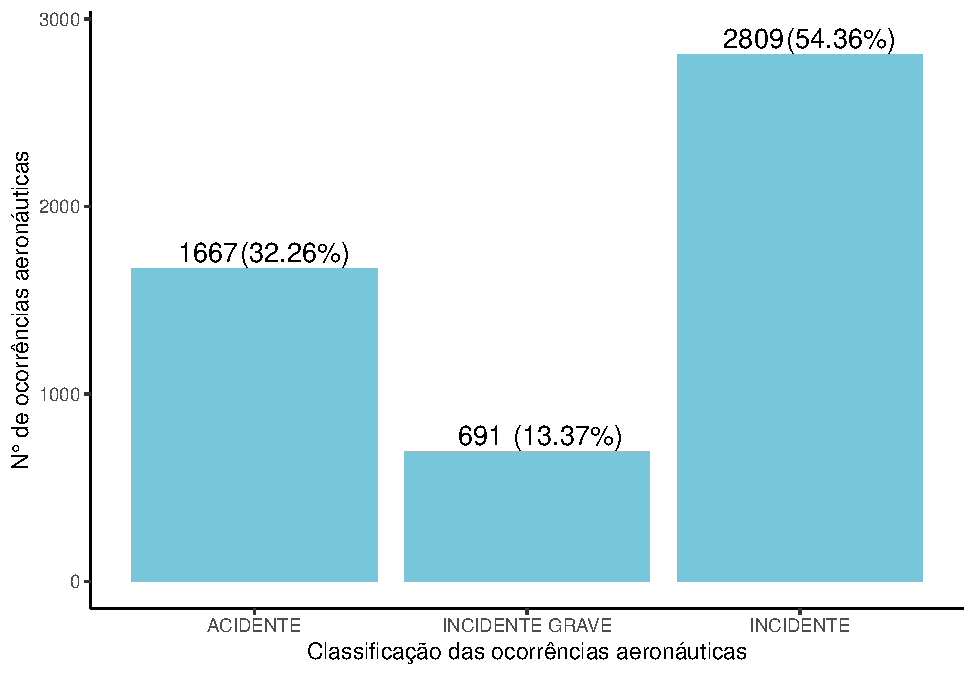
\includegraphics{4.Relatorio/pdf/index_files/figure-latex/unnamed-chunk-18-1} \end{center}

\begin{quote}
Apesar de incidentes (\textasciitilde{} 54.4\%) ocorrerem mais do que
incidentes graves ou acidentes (\textasciitilde{} 45.6\%), este último
número ainda é preocupante. O ideal é que se tenha uma porcentagem mais
baixa de incidentes graves e acidentes pois essas são mais danosas.
\end{quote}

\hypertarget{q2-o-nuxfamero-de-acidentes-tem-cauxeddo-com-o-passar-do-tempo}{%
\subsection{Q2 -- O número de acidentes tem caído com o passar do
tempo?}\label{q2-o-nuxfamero-de-acidentes-tem-cauxeddo-com-o-passar-do-tempo}}

\begin{Shaded}
\begin{Highlighting}[]
\CommentTok{\#source(\textquotesingle{}funcoes\_auxiliares/funcoes\_analiseunivariada.R\textquotesingle{},encoding="UTF{-}8")}
\NormalTok{p\_ocor\_ano }\OtherTok{\textless{}{-}} \FunctionTok{calcula\_tab\_frequencia\_dplyr}\NormalTok{(}
    \AttributeTok{tabela\_de\_entrada =}\NormalTok{ (ocorrencia }\SpecialCharTok{\%\textgreater{}\%}
\NormalTok{                            dp}\SpecialCharTok{$}\FunctionTok{mutate}\NormalTok{(}\StringTok{\textasciigrave{}}\AttributeTok{ocorrencia\_ano}\StringTok{\textasciigrave{}} \OtherTok{=}\NormalTok{ dp}\SpecialCharTok{$}\FunctionTok{sql}\NormalTok{(}\StringTok{"DATE\_PART(\textquotesingle{}year\textquotesingle{}, ocorrencia\_dia)"}\NormalTok{))}
\NormalTok{                         ), }
    \AttributeTok{nome\_variavel =} \StringTok{\textasciigrave{}}\AttributeTok{ocorrencia\_ano}\StringTok{\textasciigrave{}}\NormalTok{,}
    \AttributeTok{specific\_order =}\NormalTok{ (ocorrencia }\SpecialCharTok{\%\textgreater{}\%}
\NormalTok{                          dp}\SpecialCharTok{$}\FunctionTok{mutate}\NormalTok{(}\StringTok{\textasciigrave{}}\AttributeTok{ocorrencia\_ano}\StringTok{\textasciigrave{}} \OtherTok{=}\NormalTok{ dp}\SpecialCharTok{$}\FunctionTok{sql}\NormalTok{(}\StringTok{"DATE\_PART(\textquotesingle{}year\textquotesingle{}, ocorrencia\_dia)"}\NormalTok{)) }\SpecialCharTok{\%\textgreater{}\%}
\NormalTok{                          dp}\SpecialCharTok{$}\FunctionTok{pull}\NormalTok{(}\StringTok{\textasciigrave{}}\AttributeTok{ocorrencia\_ano}\StringTok{\textasciigrave{}}\NormalTok{) }\SpecialCharTok{\%\textgreater{}\%} 
\NormalTok{                          bs}\SpecialCharTok{$}\FunctionTok{unique}\NormalTok{() }\SpecialCharTok{\%\textgreater{}\%}\NormalTok{ bs}\SpecialCharTok{$}\FunctionTok{sort}\NormalTok{())}
\NormalTok{)}

\ControlFlowTok{if}\NormalTok{ (kn}\SpecialCharTok{$}\FunctionTok{is\_html\_output}\NormalTok{()) \{}
\NormalTok{    p\_ocor\_ano}
\NormalTok{\} }\ControlFlowTok{else}\NormalTok{ \{}
\NormalTok{    p\_ocor\_ano }\SpecialCharTok{\%\textgreater{}\%}\NormalTok{ kn}\SpecialCharTok{$}\FunctionTok{kable}\NormalTok{()}
\NormalTok{\}}
\end{Highlighting}
\end{Shaded}

\begin{longtable}[]{@{}
  >{\raggedleft\arraybackslash}p{(\columnwidth - 8\tabcolsep) * \real{0.1233}}
  >{\raggedleft\arraybackslash}p{(\columnwidth - 8\tabcolsep) * \real{0.1370}}
  >{\raggedleft\arraybackslash}p{(\columnwidth - 8\tabcolsep) * \real{0.1507}}
  >{\raggedleft\arraybackslash}p{(\columnwidth - 8\tabcolsep) * \real{0.2877}}
  >{\raggedleft\arraybackslash}p{(\columnwidth - 8\tabcolsep) * \real{0.3014}}@{}}
\toprule
\begin{minipage}[b]{\linewidth}\raggedleft
Category
\end{minipage} & \begin{minipage}[b]{\linewidth}\raggedleft
Frequency
\end{minipage} & \begin{minipage}[b]{\linewidth}\raggedleft
Percentage
\end{minipage} & \begin{minipage}[b]{\linewidth}\raggedleft
Cumulative.Frequency
\end{minipage} & \begin{minipage}[b]{\linewidth}\raggedleft
Cumulative.Percentage
\end{minipage} \\
\midrule
\endhead
2012 & 647 & 12.521773 & 647 & 12.52177 \\
2013 & 654 & 12.657248 & 1301 & 25.17902 \\
2014 & 569 & 11.012193 & 1870 & 36.19121 \\
2015 & 471 & 9.115541 & 2341 & 45.30675 \\
2016 & 403 & 7.799497 & 2744 & 53.10625 \\
2017 & 433 & 8.380104 & 3177 & 61.48636 \\
2018 & 444 & 8.592994 & 3621 & 70.07935 \\
2019 & 496 & 9.599381 & 4117 & 79.67873 \\
2020 & 509 & 9.850977 & 4626 & 89.52971 \\
2021 & 541 & 10.470292 & 5167 & 100.00000 \\
\bottomrule
\end{longtable}

\begin{Shaded}
\begin{Highlighting}[]
\DocumentationTok{\#\#\#\#\#\#\#\#\#\#\#\#\#\#\#\#\#\#\#\#\#\#\#\#\#\#\#\#\#\#\#\#\#\#\#\#\#\#\#\#\#\#\#\#\#\#\#\#\#\#\#\#\#\#\#\#\#\#\#\#\#\#\#\#\#\#\#\# Cria gráfico}

\NormalTok{p\_ocor\_ano[[}\StringTok{"Category"}\NormalTok{]] }\OtherTok{\textless{}{-}} \FunctionTok{as.factor}\NormalTok{(p\_ocor\_ano[[}\StringTok{"Category"}\NormalTok{]])}

\NormalTok{ggplot2\_p\_ocor\_ano }\OtherTok{\textless{}{-}}\NormalTok{ gg}\SpecialCharTok{$}\FunctionTok{ggplot}\NormalTok{(gg}\SpecialCharTok{$}\FunctionTok{aes}\NormalTok{(}
    \AttributeTok{x =}\NormalTok{ Category,}
    \AttributeTok{y =}\NormalTok{ Frequency,}
    \AttributeTok{group =} \DecValTok{1}
\NormalTok{), }\AttributeTok{data =}\NormalTok{ p\_ocor\_ano) }\SpecialCharTok{+}
\NormalTok{    gg}\SpecialCharTok{$}\FunctionTok{geom\_point}\NormalTok{(}\AttributeTok{colour=}\StringTok{\textquotesingle{}\#022634\textquotesingle{}}\NormalTok{) }\SpecialCharTok{+}
\NormalTok{    gg}\SpecialCharTok{$}\FunctionTok{geom\_line}\NormalTok{(}\AttributeTok{colour=}\StringTok{\textquotesingle{}\#022634\textquotesingle{}}\NormalTok{) }\SpecialCharTok{+}
\NormalTok{    gg}\SpecialCharTok{$}\FunctionTok{geom\_text}\NormalTok{(gg}\SpecialCharTok{$}\FunctionTok{aes}\NormalTok{(}\AttributeTok{label=}\NormalTok{bs}\SpecialCharTok{$}\FunctionTok{paste0}\NormalTok{(bs}\SpecialCharTok{$}\FunctionTok{round}\NormalTok{(Percentage,}\DecValTok{2}\NormalTok{),}\StringTok{\textquotesingle{}\%\textquotesingle{}}\NormalTok{),}
                  \AttributeTok{y=}\NormalTok{Frequency}\FloatTok{+0.035}\SpecialCharTok{*}\NormalTok{bs}\SpecialCharTok{$}\FunctionTok{min}\NormalTok{(Frequency))) }\SpecialCharTok{+}
\NormalTok{    gg}\SpecialCharTok{$}\FunctionTok{xlab}\NormalTok{(}\StringTok{\textquotesingle{}Ano\textquotesingle{}}\NormalTok{) }\SpecialCharTok{+}
\NormalTok{    gg}\SpecialCharTok{$}\FunctionTok{ylab}\NormalTok{(}\StringTok{\textquotesingle{}N° de ocorrências aeronáuticas\textquotesingle{}}\NormalTok{) }\SpecialCharTok{+}
\NormalTok{    gg}\SpecialCharTok{$}\FunctionTok{theme\_classic}\NormalTok{() }

\DocumentationTok{\#\#\#\#\#\#\#\#\#\#\#\#\#\#\#\#\#\#\#\#\#\#\#\#\#\#\#\#\#\#\#\#\#\#\#\#\#\#\#\#\#\#\#\#\#\#\#\#\#\#\#\#\#\#\#\#\#\#\#\#\#\#\#\#\#\#\#\# Salva gráfico}

\CommentTok{\#source(\textquotesingle{}funcoes\_auxiliares/salva\_grafico.R\textquotesingle{}, encoding = "UTF{-}8")}
\FunctionTok{salva\_grafico}\NormalTok{(}\AttributeTok{ggplot2\_grafico =}\NormalTok{ ggplot2\_p\_ocor\_ano)}

\DocumentationTok{\#\#\#\#\#\#\#\#\#\#\#\#\#\#\#\#\#\#\#\#\#\#\#\#\#\#\#\#\#\#\#\#\#\#\#\#\#\#\#\#\#\#\#\#\#\#\#\#\#\#\#\#\#\#\#\#\#\#\#\#\#\#\#\#\#\#\#\# Leitura gráfico}

\CommentTok{\#source(\textquotesingle{}funcoes\_auxiliares/leitura\_grafico.R\textquotesingle{}, encoding = "UTF{-}8")}
\FunctionTok{leitura\_grafico}\NormalTok{(}\AttributeTok{ggplot2\_grafico =}\NormalTok{ ggplot2\_p\_ocor\_ano)}
\end{Highlighting}
\end{Shaded}

\begin{center}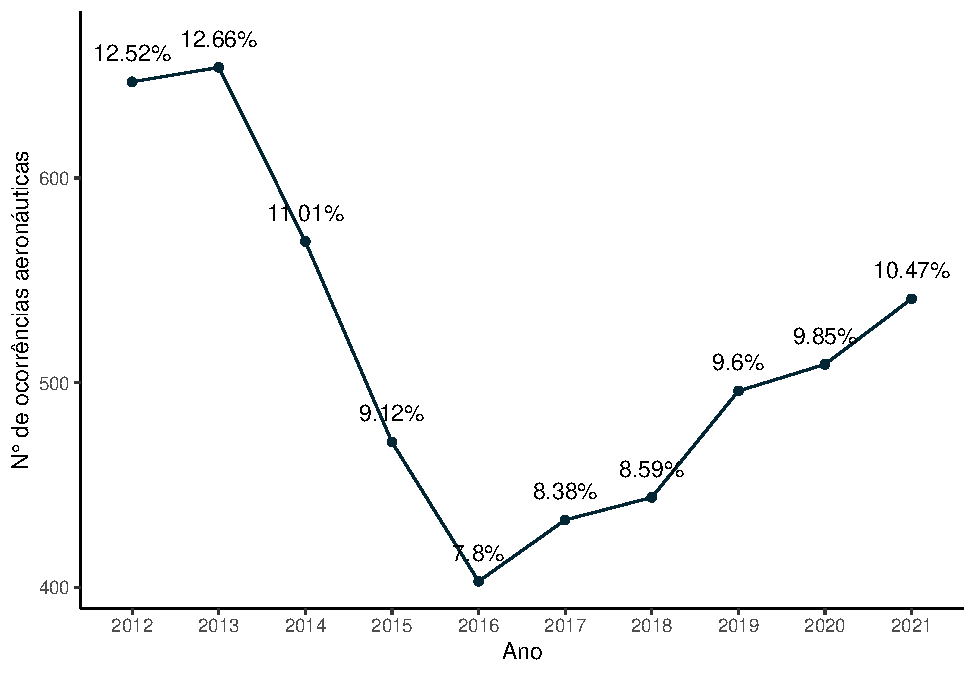
\includegraphics{4.Relatorio/pdf/index_files/figure-latex/unnamed-chunk-21-1} \end{center}

\begin{quote}
É possível perceber que o número absoluto de ocorrências aeronáuticas
teve uma queda até o ano de 2016 e voltou a subir a partir desse ano.
\end{quote}

\begin{Shaded}
\begin{Highlighting}[]
\NormalTok{ocorrencia\_aux }\OtherTok{\textless{}{-}}\NormalTok{ ocorrencia }\SpecialCharTok{\%\textgreater{}\%}
\NormalTok{    dp}\SpecialCharTok{$}\FunctionTok{mutate}\NormalTok{(}\StringTok{\textasciigrave{}}\AttributeTok{ocorrencia\_ano}\StringTok{\textasciigrave{}} \OtherTok{=}\NormalTok{ dp}\SpecialCharTok{$}\FunctionTok{sql}\NormalTok{(}\StringTok{"DATE\_PART(\textquotesingle{}year\textquotesingle{}, ocorrencia\_dia)"}\NormalTok{))}
\NormalTok{p\_ocor\_ano\_classif }\OtherTok{\textless{}{-}} \FunctionTok{calcula\_tab\_frequencia\_bivariada\_dplyr}\NormalTok{(ocorrencia\_aux,}
                                                             \StringTok{\textasciigrave{}}\AttributeTok{ocorrencia\_ano}\StringTok{\textasciigrave{}}\NormalTok{,}
                                                             \StringTok{\textasciigrave{}}\AttributeTok{ocorrencia\_classificacao}\StringTok{\textasciigrave{}}\NormalTok{)}
\end{Highlighting}
\end{Shaded}

\begin{verbatim}
## `summarise()` has grouped output by 'ocorrencia_ano'. You can override using the `.groups` argument.
\end{verbatim}

\begin{Shaded}
\begin{Highlighting}[]
\ControlFlowTok{if}\NormalTok{ (kn}\SpecialCharTok{$}\FunctionTok{is\_html\_output}\NormalTok{()) \{}
\NormalTok{    p\_ocor\_ano\_classif}
\NormalTok{\} }\ControlFlowTok{else}\NormalTok{ \{}
\NormalTok{    p\_ocor\_ano\_classif }\SpecialCharTok{\%\textgreater{}\%}\NormalTok{ kn}\SpecialCharTok{$}\FunctionTok{kable}\NormalTok{()}
\NormalTok{\}}
\end{Highlighting}
\end{Shaded}

\begin{longtable}[]{@{}
  >{\raggedleft\arraybackslash}p{(\columnwidth - 8\tabcolsep) * \real{0.2000}}
  >{\raggedright\arraybackslash}p{(\columnwidth - 8\tabcolsep) * \real{0.3333}}
  >{\raggedleft\arraybackslash}p{(\columnwidth - 8\tabcolsep) * \real{0.1333}}
  >{\raggedleft\arraybackslash}p{(\columnwidth - 8\tabcolsep) * \real{0.1867}}
  >{\raggedleft\arraybackslash}p{(\columnwidth - 8\tabcolsep) * \real{0.1467}}@{}}
\toprule
\begin{minipage}[b]{\linewidth}\raggedleft
ocorrencia\_ano
\end{minipage} & \begin{minipage}[b]{\linewidth}\raggedright
ocorrencia\_classificacao
\end{minipage} & \begin{minipage}[b]{\linewidth}\raggedleft
Frequency
\end{minipage} & \begin{minipage}[b]{\linewidth}\raggedleft
sum\_Frequency
\end{minipage} & \begin{minipage}[b]{\linewidth}\raggedleft
Percentage
\end{minipage} \\
\midrule
\endhead
2012 & INCIDENTE GRAVE & 77 & 647 & 11.90108 \\
2012 & ACIDENTE & 205 & 647 & 31.68470 \\
2012 & INCIDENTE & 365 & 647 & 56.41422 \\
2013 & ACIDENTE & 199 & 654 & 30.42813 \\
2013 & INCIDENTE GRAVE & 69 & 654 & 10.55046 \\
2013 & INCIDENTE & 386 & 654 & 59.02141 \\
2014 & INCIDENTE & 318 & 569 & 55.88752 \\
2014 & ACIDENTE & 176 & 569 & 30.93146 \\
2014 & INCIDENTE GRAVE & 75 & 569 & 13.18102 \\
2015 & INCIDENTE GRAVE & 49 & 471 & 10.40340 \\
2015 & ACIDENTE & 172 & 471 & 36.51805 \\
2015 & INCIDENTE & 250 & 471 & 53.07856 \\
2016 & INCIDENTE & 192 & 403 & 47.64268 \\
2016 & INCIDENTE GRAVE & 47 & 403 & 11.66253 \\
2016 & ACIDENTE & 164 & 403 & 40.69479 \\
2017 & ACIDENTE & 146 & 433 & 33.71824 \\
2017 & INCIDENTE GRAVE & 55 & 433 & 12.70208 \\
2017 & INCIDENTE & 232 & 433 & 53.57968 \\
2018 & INCIDENTE & 199 & 444 & 44.81982 \\
2018 & INCIDENTE GRAVE & 80 & 444 & 18.01802 \\
2018 & ACIDENTE & 165 & 444 & 37.16216 \\
2019 & INCIDENTE GRAVE & 80 & 496 & 16.12903 \\
2019 & ACIDENTE & 150 & 496 & 30.24194 \\
2019 & INCIDENTE & 266 & 496 & 53.62903 \\
2020 & INCIDENTE GRAVE & 77 & 509 & 15.12770 \\
2020 & INCIDENTE & 283 & 509 & 55.59921 \\
2020 & ACIDENTE & 149 & 509 & 29.27308 \\
2021 & ACIDENTE & 141 & 541 & 26.06285 \\
2021 & INCIDENTE & 318 & 541 & 58.78004 \\
2021 & INCIDENTE GRAVE & 82 & 541 & 15.15712 \\
\bottomrule
\end{longtable}

\begin{Shaded}
\begin{Highlighting}[]
\DocumentationTok{\#\#\#\#\#\#\#\#\#\#\#\#\#\#\#\#\#\#\#\#\#\#\#\#\#\#\#\#\#\#\#\#\#\#\#\#\#\#\#\#\#\#\#\#\#\#\#\#\#\#\#\#\#\#\#\#\#\#\#\#\#\#\#\#\#\#\#\# Cria gráfico}

\CommentTok{\# p\_ocor\_ano\_classif[["ocorrencia\_ano"]] \textless{}{-}}
\CommentTok{\#     as.factor(p\_ocor\_ano\_classif[["ocorrencia\_ano"]])}
\CommentTok{\# p\_ocor\_ano\_classif[, "ocorrencia\_classificacao"] \textless{}{-}}
\CommentTok{\#     factor(p\_ocor\_ano\_classif[, "ocorrencia\_classificacao"],}
\CommentTok{\#                    levels=c("ACIDENTE","INCIDENTE GRAVE", "INCIDENTE"))}

\NormalTok{ggplot2\_ocor\_ano\_classif }\OtherTok{\textless{}{-}}\NormalTok{ gg}\SpecialCharTok{$}\FunctionTok{ggplot}\NormalTok{(}
\NormalTok{    gg}\SpecialCharTok{$}\FunctionTok{aes}\NormalTok{(}
        \AttributeTok{x =}\NormalTok{ ocorrencia\_ano,}
        \AttributeTok{y =}\NormalTok{ Frequency,}
        \AttributeTok{colour =}\NormalTok{ ocorrencia\_classificacao,}
        \AttributeTok{group =}\NormalTok{ ocorrencia\_classificacao}
\NormalTok{    ),}
    \AttributeTok{data =}\NormalTok{ p\_ocor\_ano\_classif}
\NormalTok{) }\SpecialCharTok{+}
\NormalTok{    gg}\SpecialCharTok{$}\FunctionTok{geom\_point}\NormalTok{() }\SpecialCharTok{+}
\NormalTok{    gg}\SpecialCharTok{$}\FunctionTok{geom\_line}\NormalTok{() }\SpecialCharTok{+}
\NormalTok{    gg}\SpecialCharTok{$}\FunctionTok{ylab}\NormalTok{(}\StringTok{\textquotesingle{}N° de ocorrências aeronáuticas\textquotesingle{}}\NormalTok{) }\SpecialCharTok{+}
\NormalTok{    gg}\SpecialCharTok{$}\FunctionTok{scale\_fill\_discrete}\NormalTok{(}\AttributeTok{name =} \StringTok{"Classificação das ocorrências aeronáuticas"}\NormalTok{) }\SpecialCharTok{+}
\NormalTok{    gg}\SpecialCharTok{$}\FunctionTok{theme\_classic}\NormalTok{() }\SpecialCharTok{+}
\NormalTok{    gg}\SpecialCharTok{$}\FunctionTok{geom\_text}\NormalTok{(gg}\SpecialCharTok{$}\FunctionTok{aes}\NormalTok{(}\AttributeTok{label =}\NormalTok{ bs}\SpecialCharTok{$}\FunctionTok{paste0}\NormalTok{(bs}\SpecialCharTok{$}\FunctionTok{round}\NormalTok{(Percentage, }\DecValTok{1}\NormalTok{), }\StringTok{"\%"}\NormalTok{),}
                                    \AttributeTok{y =}\NormalTok{ bs}\SpecialCharTok{$}\FunctionTok{as.numeric}\NormalTok{(Frequency) }\SpecialCharTok{+} \DecValTok{20}\NormalTok{)) }\SpecialCharTok{+}
\NormalTok{    gg}\SpecialCharTok{$}\FunctionTok{labs}\NormalTok{(}\AttributeTok{color=}\StringTok{\textquotesingle{}Classificação das ocorr. aeron.\textquotesingle{}}\NormalTok{) }\SpecialCharTok{+}
\NormalTok{    gg}\SpecialCharTok{$}\FunctionTok{theme}\NormalTok{(}\AttributeTok{legend.position=}\StringTok{"top"}\NormalTok{) }\SpecialCharTok{+}
\NormalTok{    gg}\SpecialCharTok{$}\FunctionTok{expand\_limits}\NormalTok{(}\AttributeTok{y =}\NormalTok{ bs}\SpecialCharTok{$}\FunctionTok{max}\NormalTok{(p\_ocor\_ano\_classif[[}\StringTok{\textquotesingle{}Frequency\textquotesingle{}}\NormalTok{]]) }\SpecialCharTok{*} \FloatTok{1.2}\NormalTok{) }\SpecialCharTok{+}
\NormalTok{    gg}\SpecialCharTok{$}\FunctionTok{scale\_x\_continuous}\NormalTok{(}
        \AttributeTok{name=}\StringTok{"Ano"}\NormalTok{,}
        \AttributeTok{labels =} \FunctionTok{as.character}\NormalTok{(}\FunctionTok{unique}\NormalTok{(p\_ocor\_ano\_classif}\SpecialCharTok{$}\NormalTok{ocorrencia\_ano)),}
        \AttributeTok{breaks =} \FunctionTok{unique}\NormalTok{(p\_ocor\_ano\_classif}\SpecialCharTok{$}\NormalTok{ocorrencia\_ano)}
\NormalTok{    )}


\DocumentationTok{\#\#\#\#\#\#\#\#\#\#\#\#\#\#\#\#\#\#\#\#\#\#\#\#\#\#\#\#\#\#\#\#\#\#\#\#\#\#\#\#\#\#\#\#\#\#\#\#\#\#\#\#\#\#\#\#\#\#\#\#\#\#\#\#\#\#\#\# Salva gráfico}

\CommentTok{\#source(\textquotesingle{}funcoes\_auxiliares/salva\_grafico.R\textquotesingle{}, encoding = "UTF{-}8")}
\FunctionTok{salva\_grafico}\NormalTok{(}\AttributeTok{ggplot2\_grafico =}\NormalTok{ ggplot2\_ocor\_ano\_classif)}

\DocumentationTok{\#\#\#\#\#\#\#\#\#\#\#\#\#\#\#\#\#\#\#\#\#\#\#\#\#\#\#\#\#\#\#\#\#\#\#\#\#\#\#\#\#\#\#\#\#\#\#\#\#\#\#\#\#\#\#\#\#\#\#\#\#\#\#\#\#\#\#\# Leitura gráfico}

\CommentTok{\#source(\textquotesingle{}funcoes\_auxiliares/leitura\_grafico.R\textquotesingle{}, encoding = "UTF{-}8")}
\FunctionTok{leitura\_grafico}\NormalTok{(}\AttributeTok{ggplot2\_grafico =}\NormalTok{ ggplot2\_ocor\_ano\_classif)}
\end{Highlighting}
\end{Shaded}

\begin{center}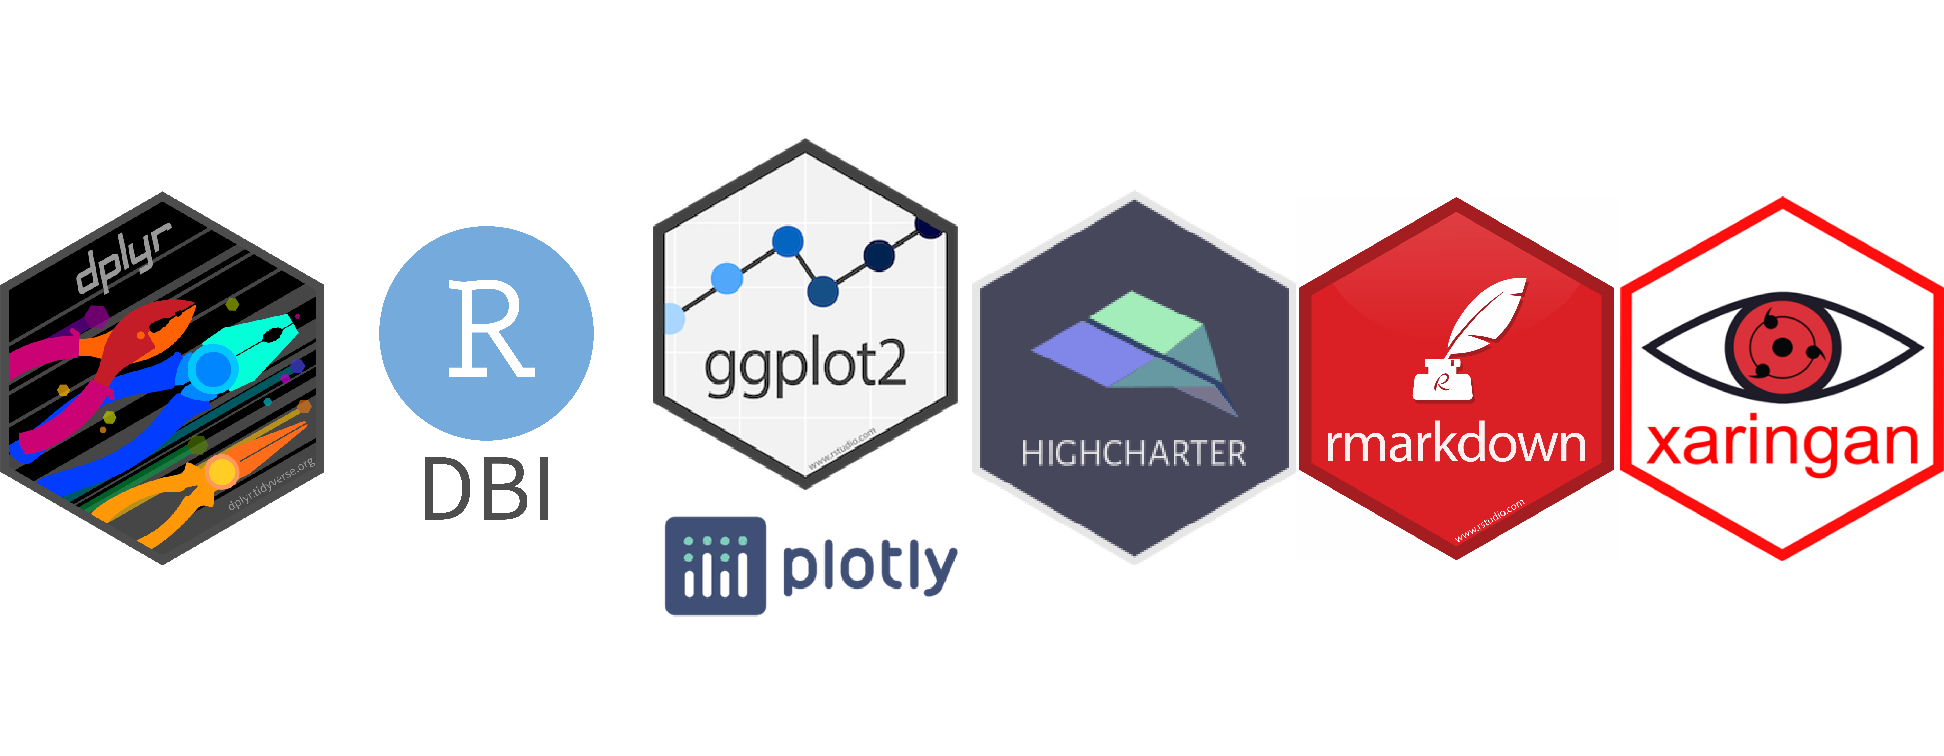
\includegraphics{4.Relatorio/pdf/index_files/figure-latex/unnamed-chunk-23-1} \end{center}

\begin{Shaded}
\begin{Highlighting}[]
\NormalTok{ggplot2\_ocor\_ano\_classif\_lm }\OtherTok{\textless{}{-}}\NormalTok{ ggplot2\_ocor\_ano\_classif}
\NormalTok{ggplot2\_ocor\_ano\_classif\_lm}\SpecialCharTok{$}\NormalTok{layers[[}\DecValTok{2}\NormalTok{]] }\OtherTok{\textless{}{-}} \ConstantTok{NULL} \CommentTok{\# remove gg$geom\_line()}
\NormalTok{ggplot2\_ocor\_ano\_classif\_lm }\OtherTok{\textless{}{-}}\NormalTok{ ggplot2\_ocor\_ano\_classif\_lm }\SpecialCharTok{+} 
\NormalTok{    gg}\SpecialCharTok{$}\FunctionTok{geom\_smooth}\NormalTok{(}\AttributeTok{data =}\NormalTok{ p\_ocor\_ano\_classif[p\_ocor\_ano\_classif}\SpecialCharTok{$}\NormalTok{ocorrencia\_ano }\SpecialCharTok{\textless{}=} \DecValTok{2016}\NormalTok{, ],}
                   \AttributeTok{method =}\NormalTok{ sta}\SpecialCharTok{$}\StringTok{"lm"}\NormalTok{,}
                   \AttributeTok{se =}\NormalTok{ F,}\AttributeTok{lwd=}\FloatTok{0.5}\NormalTok{) }\SpecialCharTok{+} \CommentTok{\# acrescenta regressão linear por partes (Ano \textless{}= 2016)}
\NormalTok{    gg}\SpecialCharTok{$}\FunctionTok{geom\_smooth}\NormalTok{(}\AttributeTok{data =}\NormalTok{ p\_ocor\_ano\_classif[p\_ocor\_ano\_classif}\SpecialCharTok{$}\NormalTok{ocorrencia\_ano }\SpecialCharTok{\textgreater{}} \DecValTok{2016}\NormalTok{,],}
                   \AttributeTok{method =}\NormalTok{ sta}\SpecialCharTok{$}\StringTok{"lm"}\NormalTok{,}
                   \AttributeTok{se =}\NormalTok{ F,}\AttributeTok{lwd=}\FloatTok{0.5}\NormalTok{) }\CommentTok{\# acrescenta regressão linear por partes (Ano \textgreater{} 2016)}
\DocumentationTok{\#\#\#\#\#\#\#\#\#\#\#\#\#\#\#\#\#\#\#\#\#\#\#\#\#\#\#\#\#\#\#\#\#\#\#\#\#\#\#\#\#\#\#\#\#\#\#\#\#\#\#\#\#\#\#\#\#\#\#\#\#\#\#\#\#\#\#\# Salva gráfico}

\CommentTok{\#source(\textquotesingle{}funcoes\_auxiliares/salva\_grafico.R\textquotesingle{}, encoding = "UTF{-}8")}
\FunctionTok{salva\_grafico}\NormalTok{(}\AttributeTok{ggplot2\_grafico =}\NormalTok{ ggplot2\_ocor\_ano\_classif\_lm)}

\DocumentationTok{\#\#\#\#\#\#\#\#\#\#\#\#\#\#\#\#\#\#\#\#\#\#\#\#\#\#\#\#\#\#\#\#\#\#\#\#\#\#\#\#\#\#\#\#\#\#\#\#\#\#\#\#\#\#\#\#\#\#\#\#\#\#\#\#\#\#\#\# Leitura gráfico}

\CommentTok{\#source(\textquotesingle{}funcoes\_auxiliares/leitura\_grafico.R\textquotesingle{}, encoding = "UTF{-}8")}
\FunctionTok{leitura\_grafico}\NormalTok{(}\AttributeTok{ggplot2\_grafico =}\NormalTok{ ggplot2\_ocor\_ano\_classif\_lm)}
\end{Highlighting}
\end{Shaded}

\begin{center}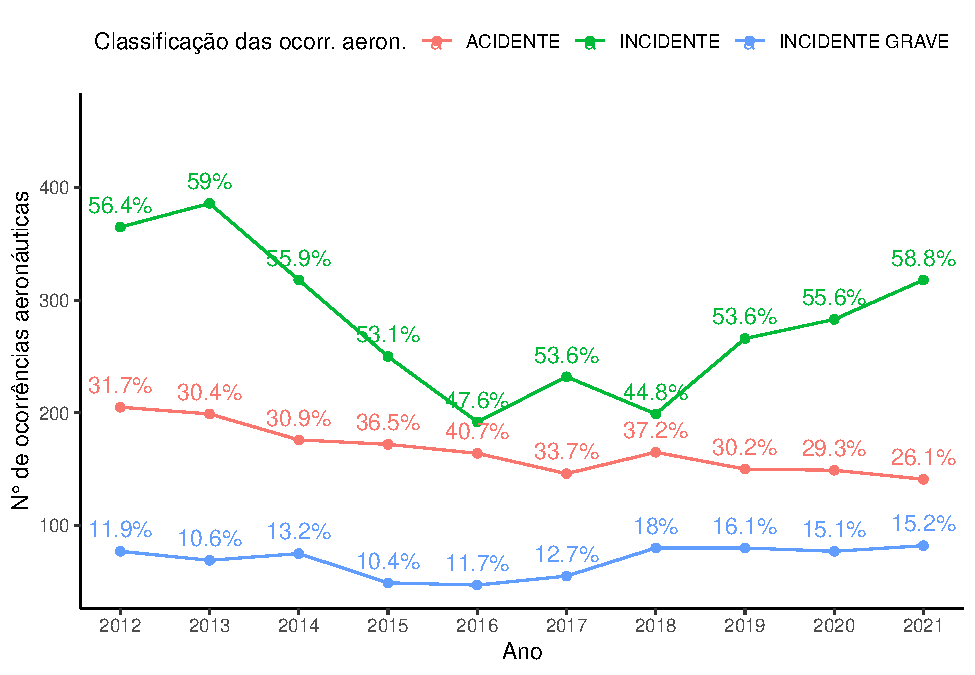
\includegraphics{4.Relatorio/pdf/index_files/figure-latex/unnamed-chunk-24-1} \end{center}

\begin{quote}
Nota-se que a tendência geral do número absoluto de ocorrências
aeronáuticas também ocorre nas ocorrências de classificação do tipo
``INCIDENTE'' e em menor grau na classificação do tipo ``INCIDENTE
GRAVE'', ou seja, há presença de tendência de baixa até 2016 e de alta
após o mesmo ano. Comportamento diferente é observado na tendência do
número de ocorrências aeronáuticas com classificação do tipo
``ACIDENTE'' que se manteve em queda desde 2012. Além disso, é
importante ressaltar que as somas das frequências relativas de
``ACIDENTES'' e ``INCIDENTES GRAVES'' ao longo dos anos variaram com
valores mínimo e máximo iguais à 41\% em 2013 e 55.2\% em 2018,
respectivamente.
\end{quote}

\hypertarget{q3-ocorrem-mais-acidentes-em-estados-de-maior-atividade-econuxf4mica-ex.-sp-mg-rj-pr}{%
\subsection{Q3 -- Ocorrem mais acidentes em estados de maior atividade
econômica (Ex.: SP, MG, RJ,
PR)?}\label{q3-ocorrem-mais-acidentes-em-estados-de-maior-atividade-econuxf4mica-ex.-sp-mg-rj-pr}}

\begin{Shaded}
\begin{Highlighting}[]
\NormalTok{p\_ocor\_uf }\OtherTok{\textless{}{-}} \FunctionTok{calcula\_tab\_frequencia\_dplyr}\NormalTok{(}
    \AttributeTok{tabela\_de\_entrada =}\NormalTok{ ocorrencia,}
    \AttributeTok{nome\_variavel =} \StringTok{\textasciigrave{}}\AttributeTok{ocorrencia\_uf}\StringTok{\textasciigrave{}}
\NormalTok{)}

\NormalTok{p\_ocor\_uf[,}\StringTok{\textquotesingle{}Category\textquotesingle{}}\NormalTok{] }\OtherTok{\textless{}{-}} \FunctionTok{as.character}\NormalTok{(p\_ocor\_uf[,}\StringTok{\textquotesingle{}Category\textquotesingle{}}\NormalTok{],}\DecValTok{2}\NormalTok{)}
\NormalTok{p\_ocor\_uf[,}\StringTok{\textquotesingle{}Percentage\textquotesingle{}}\NormalTok{] }\OtherTok{\textless{}{-}} \FunctionTok{round}\NormalTok{(p\_ocor\_uf[,}\StringTok{\textquotesingle{}Percentage\textquotesingle{}}\NormalTok{],}\DecValTok{2}\NormalTok{)}

\ControlFlowTok{if}\NormalTok{ (kn}\SpecialCharTok{$}\FunctionTok{is\_html\_output}\NormalTok{()) \{}
\NormalTok{    p\_ocor\_uf}
\NormalTok{\} }\ControlFlowTok{else}\NormalTok{ \{}
\NormalTok{    p\_ocor\_uf }\SpecialCharTok{\%\textgreater{}\%}\NormalTok{ kn}\SpecialCharTok{$}\FunctionTok{kable}\NormalTok{()}
\NormalTok{\}}
\end{Highlighting}
\end{Shaded}

\begin{longtable}[]{@{}
  >{\raggedright\arraybackslash}p{(\columnwidth - 8\tabcolsep) * \real{0.1233}}
  >{\raggedleft\arraybackslash}p{(\columnwidth - 8\tabcolsep) * \real{0.1370}}
  >{\raggedleft\arraybackslash}p{(\columnwidth - 8\tabcolsep) * \real{0.1507}}
  >{\raggedleft\arraybackslash}p{(\columnwidth - 8\tabcolsep) * \real{0.2877}}
  >{\raggedleft\arraybackslash}p{(\columnwidth - 8\tabcolsep) * \real{0.3014}}@{}}
\toprule
\begin{minipage}[b]{\linewidth}\raggedright
Category
\end{minipage} & \begin{minipage}[b]{\linewidth}\raggedleft
Frequency
\end{minipage} & \begin{minipage}[b]{\linewidth}\raggedleft
Percentage
\end{minipage} & \begin{minipage}[b]{\linewidth}\raggedleft
Cumulative.Frequency
\end{minipage} & \begin{minipage}[b]{\linewidth}\raggedleft
Cumulative.Percentage
\end{minipage} \\
\midrule
\endhead
RR & 54 & 1.05 & 54 & 1.045094 \\
MG & 499 & 9.66 & 553 & 10.702535 \\
MT & 276 & 5.34 & 829 & 16.044126 \\
CE & 78 & 1.51 & 907 & 17.553706 \\
AC & 49 & 0.95 & 956 & 18.502032 \\
RS & 327 & 6.33 & 1283 & 24.830656 \\
DF & 106 & 2.05 & 1389 & 26.882137 \\
SP & 1261 & 24.40 & 2650 & 51.287014 \\
AP & 12 & 0.23 & 2662 & 51.519257 \\
ES & 73 & 1.41 & 2735 & 52.932069 \\
BA & 183 & 3.54 & 2918 & 56.473776 \\
MA & 59 & 1.14 & 2977 & 57.615638 \\
AL & 28 & 0.54 & 3005 & 58.157538 \\
RN & 17 & 0.33 & 3022 & 58.486549 \\
PE & 86 & 1.66 & 3108 & 60.150958 \\
RJ & 402 & 7.78 & 3510 & 67.931101 \\
SE & 14 & 0.27 & 3524 & 68.202051 \\
SC & 167 & 3.23 & 3691 & 71.434101 \\
GO & 268 & 5.19 & 3959 & 76.620863 \\
PB & 22 & 0.43 & 3981 & 77.046642 \\
PI & 38 & 0.74 & 4019 & 77.782079 \\
PR & 431 & 8.34 & 4450 & 86.123476 \\
RO & 43 & 0.83 & 4493 & 86.955680 \\
MS & 158 & 3.06 & 4651 & 90.013548 \\
*** & 2 & 0.04 & 4653 & 90.052255 \\
AM & 207 & 4.01 & 4860 & 94.058448 \\
PA & 261 & 5.05 & 5121 & 99.109735 \\
TO & 46 & 0.89 & 5167 & 100.000000 \\
\bottomrule
\end{longtable}

\begin{Shaded}
\begin{Highlighting}[]
\CommentTok{\# se der erro parecido com:}
\CommentTok{\# Error: parse error: trailing garbage}
\CommentTok{\#          [2804,4640],[2713,4570]]]\}\}]\};}
\CommentTok{\#                     (right here) {-}{-}{-}{-}{-}{-}\^{}}
\CommentTok{\# instalar pacote com remotes::install\_github("jbkunst/highcharter")}
\CommentTok{\# e tentar novamente}

\CommentTok{\#remotes::install\_github("jbkunst/highcharter")}
\CommentTok{\#library(highcharter)}

\ControlFlowTok{if}\NormalTok{ (}\FunctionTok{file.exists}\NormalTok{(bs}\SpecialCharTok{$}\FunctionTok{paste0}\NormalTok{(endereco\_graficos\_interativos, }\StringTok{"map.rds"}\NormalTok{))) \{}
\NormalTok{    map }\OtherTok{\textless{}{-}}\NormalTok{ bs}\SpecialCharTok{$}\FunctionTok{readRDS}\NormalTok{(}\AttributeTok{file =}\NormalTok{ bs}\SpecialCharTok{$}\FunctionTok{paste0}\NormalTok{(endereco\_graficos\_interativos, }\StringTok{"map.rds"}\NormalTok{))}
\NormalTok{\} }\ControlFlowTok{else}\NormalTok{ \{}
\NormalTok{    map }\OtherTok{\textless{}{-}}\NormalTok{ hc}\SpecialCharTok{$}\FunctionTok{get\_data\_from\_map}\NormalTok{(hc}\SpecialCharTok{$}\FunctionTok{download\_map\_data}\NormalTok{(}\StringTok{"countries/br/br{-}all"}\NormalTok{))}
\NormalTok{\}}

\ControlFlowTok{if}\NormalTok{ (}\FunctionTok{file.exists}\NormalTok{(bs}\SpecialCharTok{$}\FunctionTok{paste0}\NormalTok{(endereco\_graficos\_interativos, }\StringTok{"map2.rds"}\NormalTok{))) \{}
\NormalTok{    map2 }\OtherTok{\textless{}{-}}\NormalTok{ bs}\SpecialCharTok{$}\FunctionTok{readRDS}\NormalTok{(}\AttributeTok{file =}\NormalTok{ bs}\SpecialCharTok{$}\FunctionTok{paste0}\NormalTok{(endereco\_graficos\_interativos, }\StringTok{"map2.rds"}\NormalTok{))}
\NormalTok{\} }\ControlFlowTok{else}\NormalTok{ \{}
\NormalTok{    map2 }\OtherTok{\textless{}{-}}\NormalTok{ hc}\SpecialCharTok{$}\FunctionTok{download\_map\_data}\NormalTok{(}\StringTok{"countries/br/br{-}all"}\NormalTok{)}
\NormalTok{\}}

\NormalTok{bs}\SpecialCharTok{$}\FunctionTok{saveRDS}\NormalTok{(}
\NormalTok{    map,}
    \AttributeTok{file =}\NormalTok{ bs}\SpecialCharTok{$}\FunctionTok{paste0}\NormalTok{(}
\NormalTok{        endereco\_graficos\_interativos,}
        \StringTok{"map.rds"}
\NormalTok{    )}
\NormalTok{)}
\NormalTok{bs}\SpecialCharTok{$}\FunctionTok{saveRDS}\NormalTok{(}
\NormalTok{    map2,}
    \AttributeTok{file =}\NormalTok{ bs}\SpecialCharTok{$}\FunctionTok{paste0}\NormalTok{(}
\NormalTok{        endereco\_graficos\_interativos,}
        \StringTok{"map2.rds"}
\NormalTok{    )}
\NormalTok{)}

\NormalTok{dados }\OtherTok{\textless{}{-}}\NormalTok{ map[,bs}\SpecialCharTok{$}\FunctionTok{c}\NormalTok{(}\StringTok{"woe{-}name"}\NormalTok{,}\StringTok{"hc{-}a2"}\NormalTok{)] }\SpecialCharTok{\%\textgreater{}\%} 
\NormalTok{    dp}\SpecialCharTok{$}\FunctionTok{left\_join}\NormalTok{(}\AttributeTok{x=}\NormalTok{.,}\AttributeTok{y=}\NormalTok{p\_ocor\_uf, }\AttributeTok{by =}\NormalTok{ bs}\SpecialCharTok{$}\FunctionTok{c}\NormalTok{(}\StringTok{"hc{-}a2"} \OtherTok{=} \StringTok{"Category"}\NormalTok{))}
\end{Highlighting}
\end{Shaded}

\begin{Shaded}
\begin{Highlighting}[]
\CommentTok{\# instalar phantomjs se gráfico não ser gerado em pdf}
\CommentTok{\# webshot::install\_phantomjs()}


\NormalTok{plot }\OtherTok{\textless{}{-}}\NormalTok{ hc}\SpecialCharTok{$}\FunctionTok{highchart}\NormalTok{(}\AttributeTok{type =} \StringTok{"map"}\NormalTok{) }\SpecialCharTok{\%\textgreater{}\%}
    \CommentTok{\#hc$hc\_plotOptions(series = list(animation = FALSE)) \%\textgreater{}\% }
\NormalTok{  hc}\SpecialCharTok{$}\FunctionTok{hc\_add\_series\_map}\NormalTok{(}\AttributeTok{map =}\NormalTok{ map2,}
                    \AttributeTok{df =}\NormalTok{ dados,}
                    \AttributeTok{value =} \StringTok{"Frequency"}\NormalTok{,}
                    \AttributeTok{joinBy =} \StringTok{"hc{-}a2"}\NormalTok{,}
                        \AttributeTok{dataLabels =}\NormalTok{ bs}\SpecialCharTok{$}\FunctionTok{list}\NormalTok{(}
                          \AttributeTok{enabled =} \ConstantTok{TRUE}\NormalTok{,}
                          \AttributeTok{format =} \StringTok{"\{point.hc{-}a2\}"}
\NormalTok{                          )) }\SpecialCharTok{\%\textgreater{}\%}
\NormalTok{    hc}\SpecialCharTok{$}\FunctionTok{hc\_tooltip}\NormalTok{(}
    \AttributeTok{useHTML =} \ConstantTok{TRUE}\NormalTok{, }\AttributeTok{headerFormat =} \StringTok{""}\NormalTok{,}
    \AttributeTok{pointFormat =} \StringTok{"\{point.name\} {-} \{point.value\} (\{point.Percentage\}\%)"}
\NormalTok{  ) }\SpecialCharTok{\%\textgreater{}\%} 
\NormalTok{  hc}\SpecialCharTok{$}\FunctionTok{hc\_title}\NormalTok{(}\AttributeTok{text =} \StringTok{"Ocorrências aeronáuticas por unidade federativa"}\NormalTok{)}



\NormalTok{hw}\SpecialCharTok{$}\FunctionTok{saveWidget}\NormalTok{(}\AttributeTok{widget =}\NormalTok{ plot, }\AttributeTok{file =} \FunctionTok{paste0}\NormalTok{(endereco\_imagens,}\StringTok{"plot.html"}\NormalTok{))}
\ControlFlowTok{if}\NormalTok{ (kn}\SpecialCharTok{$}\FunctionTok{is\_html\_output}\NormalTok{()) \{}
\NormalTok{    plot}
\NormalTok{\} }\ControlFlowTok{else}\NormalTok{ \{}
\NormalTok{    wb}\SpecialCharTok{$}\FunctionTok{webshot}\NormalTok{(}\AttributeTok{url =} \FunctionTok{paste0}\NormalTok{(endereco\_imagens,}\StringTok{"plot.html"}\NormalTok{), }
                     \AttributeTok{file =}\FunctionTok{paste0}\NormalTok{(endereco\_imagens,}\StringTok{"plot.png"}\NormalTok{),}
                     \AttributeTok{delay =} \FloatTok{0.2}\NormalTok{,}
                     \AttributeTok{zoom=}\FloatTok{1.5}\NormalTok{)}
\NormalTok{\}}
\end{Highlighting}
\end{Shaded}

\begin{center}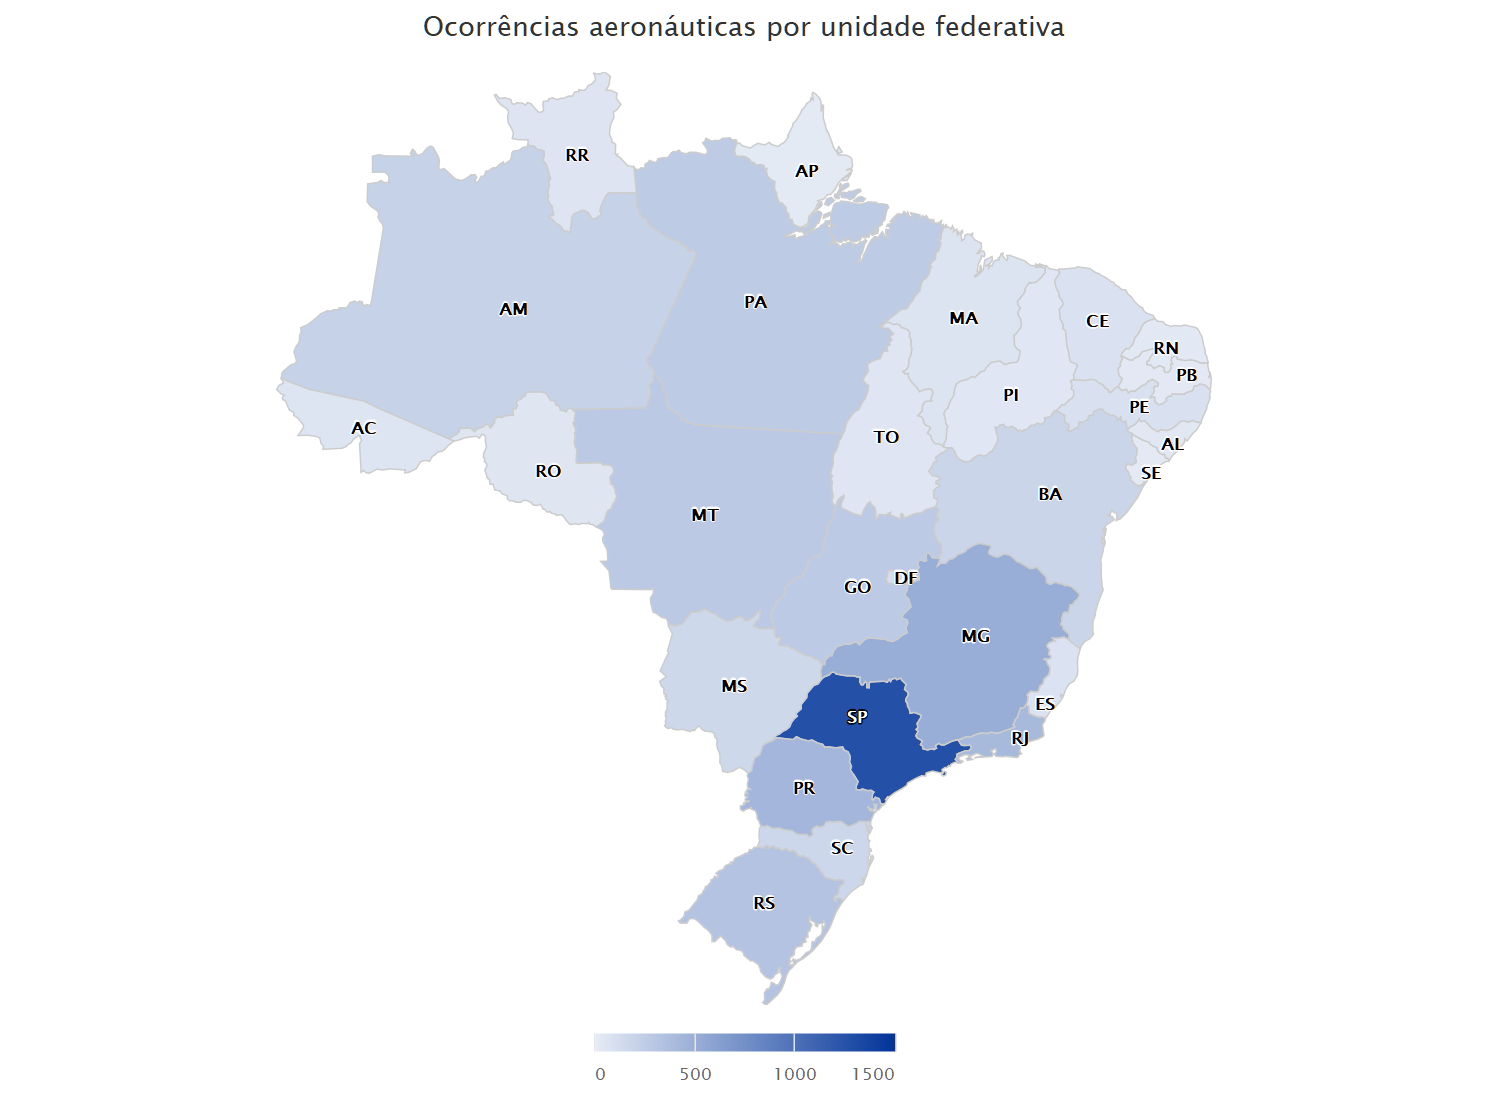
\includegraphics{4.Relatorio/pdf/index_files/figure-latex/unnamed-chunk-28-1} \end{center}

\begin{Shaded}
\begin{Highlighting}[]
\NormalTok{bs}\SpecialCharTok{$}\FunctionTok{saveRDS}\NormalTok{(plot,}
           \AttributeTok{file =}\NormalTok{ bs}\SpecialCharTok{$}\FunctionTok{paste0}\NormalTok{(endereco\_graficos\_interativos,}
                            \FunctionTok{substitute}\NormalTok{(plot),}
                            \StringTok{".rds"}\NormalTok{))}
\end{Highlighting}
\end{Shaded}

\begin{Shaded}
\begin{Highlighting}[]
\NormalTok{p\_ocor\_uf\_classif }\OtherTok{\textless{}{-}} \FunctionTok{calcula\_tab\_frequencia\_bivariada\_dplyr}\NormalTok{(ocorrencia\_aux,}
                                                             \StringTok{\textasciigrave{}}\AttributeTok{ocorrencia\_uf}\StringTok{\textasciigrave{}}\NormalTok{,}
                                                             \StringTok{\textasciigrave{}}\AttributeTok{ocorrencia\_classificacao}\StringTok{\textasciigrave{}}\NormalTok{)}
\end{Highlighting}
\end{Shaded}

\begin{verbatim}
## `summarise()` has grouped output by 'ocorrencia_uf'. You can override using the `.groups` argument.
\end{verbatim}

\begin{Shaded}
\begin{Highlighting}[]
\NormalTok{p\_ocor\_uf\_classif }\OtherTok{\textless{}{-}}\NormalTok{ p\_ocor\_uf\_classif }\SpecialCharTok{\%\textgreater{}\%}\NormalTok{ dp}\SpecialCharTok{$}\FunctionTok{arrange}\NormalTok{(dp}\SpecialCharTok{$}\FunctionTok{desc}\NormalTok{(sum\_Frequency))}
\NormalTok{p\_ocor\_uf\_classif}\SpecialCharTok{$}\StringTok{\textasciigrave{}}\AttributeTok{Percentage}\StringTok{\textasciigrave{}} \OtherTok{\textless{}{-}} \FunctionTok{round}\NormalTok{(p\_ocor\_uf\_classif}\SpecialCharTok{$}\StringTok{\textasciigrave{}}\AttributeTok{Percentage}\StringTok{\textasciigrave{}}\NormalTok{,}\DecValTok{1}\NormalTok{)}
\NormalTok{p\_ocor\_uf\_classif}\SpecialCharTok{$}\StringTok{\textasciigrave{}}\AttributeTok{ocorrencia\_uf}\StringTok{\textasciigrave{}} \OtherTok{\textless{}{-}}\NormalTok{ fc}\SpecialCharTok{$}\FunctionTok{fct\_inorder}\NormalTok{(p\_ocor\_uf\_classif}\SpecialCharTok{$}\StringTok{\textasciigrave{}}\AttributeTok{ocorrencia\_uf}\StringTok{\textasciigrave{}}\NormalTok{)}

\ControlFlowTok{if}\NormalTok{ (kn}\SpecialCharTok{$}\FunctionTok{is\_html\_output}\NormalTok{()) \{}
\NormalTok{    p\_ocor\_uf\_classif}
\NormalTok{\} }\ControlFlowTok{else}\NormalTok{ \{}
\NormalTok{    p\_ocor\_uf\_classif }\SpecialCharTok{\%\textgreater{}\%}\NormalTok{ kn}\SpecialCharTok{$}\FunctionTok{kable}\NormalTok{()}
\NormalTok{\}}
\end{Highlighting}
\end{Shaded}

\begin{longtable}[]{@{}
  >{\raggedright\arraybackslash}p{(\columnwidth - 8\tabcolsep) * \real{0.1892}}
  >{\raggedright\arraybackslash}p{(\columnwidth - 8\tabcolsep) * \real{0.3378}}
  >{\raggedleft\arraybackslash}p{(\columnwidth - 8\tabcolsep) * \real{0.1351}}
  >{\raggedleft\arraybackslash}p{(\columnwidth - 8\tabcolsep) * \real{0.1892}}
  >{\raggedleft\arraybackslash}p{(\columnwidth - 8\tabcolsep) * \real{0.1486}}@{}}
\toprule
\begin{minipage}[b]{\linewidth}\raggedright
ocorrencia\_uf
\end{minipage} & \begin{minipage}[b]{\linewidth}\raggedright
ocorrencia\_classificacao
\end{minipage} & \begin{minipage}[b]{\linewidth}\raggedleft
Frequency
\end{minipage} & \begin{minipage}[b]{\linewidth}\raggedleft
sum\_Frequency
\end{minipage} & \begin{minipage}[b]{\linewidth}\raggedleft
Percentage
\end{minipage} \\
\midrule
\endhead
SP & INCIDENTE GRAVE & 132 & 1261 & 10.5 \\
SP & ACIDENTE & 348 & 1261 & 27.6 \\
SP & INCIDENTE & 781 & 1261 & 61.9 \\
MG & INCIDENTE GRAVE & 67 & 499 & 13.4 \\
MG & ACIDENTE & 141 & 499 & 28.3 \\
MG & INCIDENTE & 291 & 499 & 58.3 \\
PR & INCIDENTE & 248 & 431 & 57.5 \\
PR & INCIDENTE GRAVE & 50 & 431 & 11.6 \\
PR & ACIDENTE & 133 & 431 & 30.9 \\
RJ & ACIDENTE & 58 & 402 & 14.4 \\
RJ & INCIDENTE GRAVE & 40 & 402 & 10.0 \\
RJ & INCIDENTE & 304 & 402 & 75.6 \\
RS & INCIDENTE GRAVE & 43 & 327 & 13.1 \\
RS & ACIDENTE & 155 & 327 & 47.4 \\
RS & INCIDENTE & 129 & 327 & 39.4 \\
MT & INCIDENTE GRAVE & 47 & 276 & 17.0 \\
MT & ACIDENTE & 157 & 276 & 56.9 \\
MT & INCIDENTE & 72 & 276 & 26.1 \\
GO & INCIDENTE & 88 & 268 & 32.8 \\
GO & ACIDENTE & 114 & 268 & 42.5 \\
GO & INCIDENTE GRAVE & 66 & 268 & 24.6 \\
PA & ACIDENTE & 117 & 261 & 44.8 \\
PA & INCIDENTE GRAVE & 38 & 261 & 14.6 \\
PA & INCIDENTE & 106 & 261 & 40.6 \\
AM & INCIDENTE & 122 & 207 & 58.9 \\
AM & ACIDENTE & 63 & 207 & 30.4 \\
AM & INCIDENTE GRAVE & 22 & 207 & 10.6 \\
BA & INCIDENTE GRAVE & 32 & 183 & 17.5 \\
BA & INCIDENTE & 99 & 183 & 54.1 \\
BA & ACIDENTE & 52 & 183 & 28.4 \\
SC & INCIDENTE GRAVE & 14 & 167 & 8.4 \\
SC & ACIDENTE & 56 & 167 & 33.5 \\
SC & INCIDENTE & 97 & 167 & 58.1 \\
MS & INCIDENTE & 54 & 158 & 34.2 \\
MS & ACIDENTE & 78 & 158 & 49.4 \\
MS & INCIDENTE GRAVE & 26 & 158 & 16.5 \\
DF & ACIDENTE & 6 & 106 & 5.7 \\
DF & INCIDENTE & 90 & 106 & 84.9 \\
DF & INCIDENTE GRAVE & 10 & 106 & 9.4 \\
PE & INCIDENTE & 63 & 86 & 73.3 \\
PE & ACIDENTE & 14 & 86 & 16.3 \\
PE & INCIDENTE GRAVE & 9 & 86 & 10.5 \\
CE & INCIDENTE GRAVE & 14 & 78 & 17.9 \\
CE & ACIDENTE & 19 & 78 & 24.4 \\
CE & INCIDENTE & 45 & 78 & 57.7 \\
ES & ACIDENTE & 13 & 73 & 17.8 \\
ES & INCIDENTE & 50 & 73 & 68.5 \\
ES & INCIDENTE GRAVE & 10 & 73 & 13.7 \\
MA & INCIDENTE GRAVE & 12 & 59 & 20.3 \\
MA & ACIDENTE & 27 & 59 & 45.8 \\
MA & INCIDENTE & 20 & 59 & 33.9 \\
RR & ACIDENTE & 30 & 54 & 55.6 \\
RR & INCIDENTE & 17 & 54 & 31.5 \\
RR & INCIDENTE GRAVE & 7 & 54 & 13.0 \\
AC & INCIDENTE & 28 & 49 & 57.1 \\
AC & ACIDENTE & 12 & 49 & 24.5 \\
AC & INCIDENTE GRAVE & 9 & 49 & 18.4 \\
TO & INCIDENTE & 17 & 46 & 37.0 \\
TO & INCIDENTE GRAVE & 10 & 46 & 21.7 \\
TO & ACIDENTE & 19 & 46 & 41.3 \\
RO & INCIDENTE GRAVE & 9 & 43 & 20.9 \\
RO & INCIDENTE & 18 & 43 & 41.9 \\
RO & ACIDENTE & 16 & 43 & 37.2 \\
PI & INCIDENTE & 17 & 38 & 44.7 \\
PI & INCIDENTE GRAVE & 7 & 38 & 18.4 \\
PI & ACIDENTE & 14 & 38 & 36.8 \\
AL & INCIDENTE GRAVE & 5 & 28 & 17.9 \\
AL & ACIDENTE & 1 & 28 & 3.6 \\
AL & INCIDENTE & 22 & 28 & 78.6 \\
PB & INCIDENTE & 10 & 22 & 45.5 \\
PB & INCIDENTE GRAVE & 5 & 22 & 22.7 \\
PB & ACIDENTE & 7 & 22 & 31.8 \\
RN & INCIDENTE GRAVE & 4 & 17 & 23.5 \\
RN & INCIDENTE & 9 & 17 & 52.9 \\
RN & ACIDENTE & 4 & 17 & 23.5 \\
SE & INCIDENTE GRAVE & 2 & 14 & 14.3 \\
SE & ACIDENTE & 7 & 14 & 50.0 \\
SE & INCIDENTE & 5 & 14 & 35.7 \\
AP & ACIDENTE & 4 & 12 & 33.3 \\
AP & INCIDENTE & 7 & 12 & 58.3 \\
AP & INCIDENTE GRAVE & 1 & 12 & 8.3 \\
*** & ACIDENTE & 2 & 2 & 100.0 \\
\bottomrule
\end{longtable}

\begin{Shaded}
\begin{Highlighting}[]
\NormalTok{ggplot2\_ocor\_uf\_classif1 }\OtherTok{\textless{}{-}} \FunctionTok{grafico\_tab\_frequencia\_bivariada2}\NormalTok{(}
\NormalTok{    p\_ocor\_uf\_classif,}
    \StringTok{"ocorrencia\_classificacao"}\NormalTok{,}
    \StringTok{"ocorrencia\_uf"}\NormalTok{,}
    \AttributeTok{tx1 =} \FloatTok{0.6}\NormalTok{,}
    \AttributeTok{tx2 =} \FloatTok{1.3}\NormalTok{,}
    \AttributeTok{size =} \DecValTok{3}\NormalTok{,}
    \AttributeTok{legend =} \ConstantTok{TRUE}
\NormalTok{) }\SpecialCharTok{+}\NormalTok{ gg}\SpecialCharTok{$}\FunctionTok{coord\_cartesian}\NormalTok{(}\AttributeTok{xlim =} \FunctionTok{c}\NormalTok{(p\_ocor\_uf\_classif[[}\StringTok{"ocorrencia\_uf"}\NormalTok{]][}\DecValTok{1}\NormalTok{],}
\NormalTok{                        p\_ocor\_uf\_classif[[}\StringTok{"ocorrencia\_uf"}\NormalTok{]][}\DecValTok{15}\NormalTok{])) }\SpecialCharTok{+}
\NormalTok{    gg}\SpecialCharTok{$}\FunctionTok{scale\_fill\_discrete}\NormalTok{(}\AttributeTok{name =} \StringTok{"Classificação das ocorr. aeron."}\NormalTok{) }\SpecialCharTok{+}
\NormalTok{    gg}\SpecialCharTok{$}\FunctionTok{theme}\NormalTok{(}\AttributeTok{legend.position=}\StringTok{"top"}\NormalTok{) }\SpecialCharTok{+} 
\NormalTok{    gg}\SpecialCharTok{$}\FunctionTok{ylab}\NormalTok{(}\StringTok{\textquotesingle{}N° de ocorrências aeronáuticas\textquotesingle{}}\NormalTok{) }\SpecialCharTok{+}
\NormalTok{    gg}\SpecialCharTok{$}\FunctionTok{xlab}\NormalTok{(}\StringTok{\textquotesingle{}UF\textquotesingle{}}\NormalTok{)}
\end{Highlighting}
\end{Shaded}

\begin{verbatim}
## [1] "Para retirar as porcentagens, use size = 0!"
\end{verbatim}

\begin{Shaded}
\begin{Highlighting}[]
\DocumentationTok{\#\#\#\#\#\#\#\#\#\#\#\#\#\#\#\#\#\#\#\#\#\#\#\#\#\#\#\#\#\#\#\#\#\#\#\#\#\#\#\#\#\#\#\#\#\#\#\#\#\#\#\#\#\#\#\#\#\#\#\#\#\#\#\#\#\#\#\# Salva gráfico}

\CommentTok{\#source(\textquotesingle{}funcoes\_auxiliares/salva\_grafico.R\textquotesingle{}, encoding = "UTF{-}8")}
\FunctionTok{salva\_grafico}\NormalTok{(}\AttributeTok{ggplot2\_grafico =}\NormalTok{ ggplot2\_ocor\_uf\_classif1)}

\DocumentationTok{\#\#\#\#\#\#\#\#\#\#\#\#\#\#\#\#\#\#\#\#\#\#\#\#\#\#\#\#\#\#\#\#\#\#\#\#\#\#\#\#\#\#\#\#\#\#\#\#\#\#\#\#\#\#\#\#\#\#\#\#\#\#\#\#\#\#\#\# Leitura gráfico}

\CommentTok{\#source(\textquotesingle{}funcoes\_auxiliares/leitura\_grafico.R\textquotesingle{}, encoding = "UTF{-}8")}
\FunctionTok{leitura\_grafico}\NormalTok{(}\AttributeTok{ggplot2\_grafico =}\NormalTok{ ggplot2\_ocor\_uf\_classif1)}
\end{Highlighting}
\end{Shaded}

\begin{center}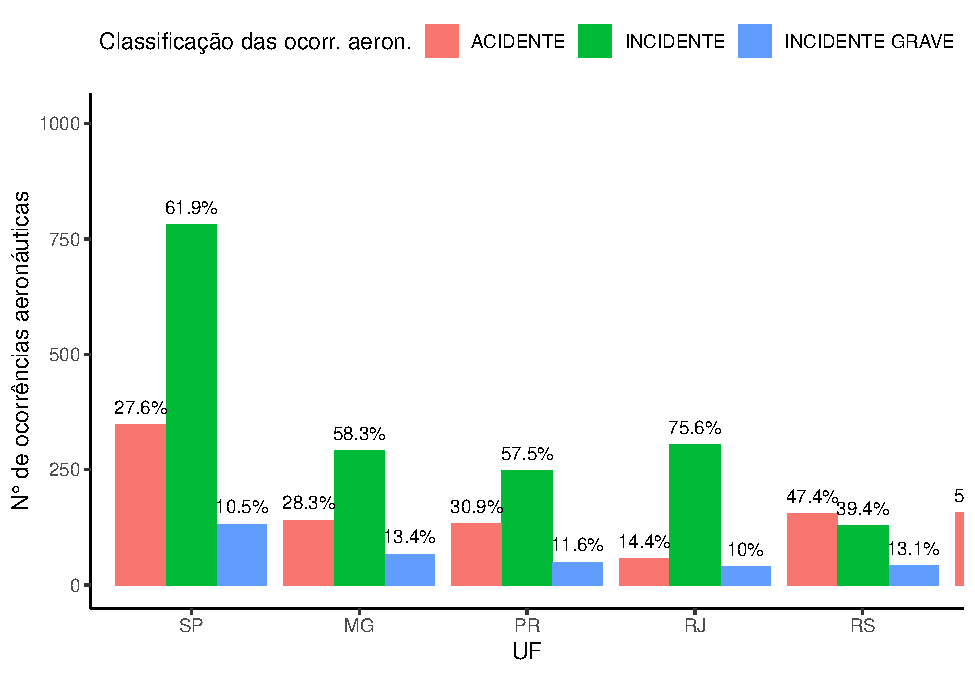
\includegraphics{4.Relatorio/pdf/index_files/figure-latex/unnamed-chunk-31-1} \end{center}

\begin{Shaded}
\begin{Highlighting}[]
\NormalTok{ggplot2\_ocor\_uf\_classif2 }\OtherTok{\textless{}{-}} \FunctionTok{grafico\_tab\_frequencia\_bivariada3}\NormalTok{(}
\NormalTok{    p\_ocor\_uf\_classif,}
    \StringTok{"ocorrencia\_classificacao"}\NormalTok{,}
    \StringTok{"ocorrencia\_uf"}\NormalTok{,}
    \AttributeTok{size =} \DecValTok{2}\NormalTok{,}
    \AttributeTok{tx1 =} \FloatTok{0.025}\NormalTok{,}
    \AttributeTok{tx2 =} \FloatTok{0.00025}\NormalTok{,}
    \AttributeTok{legend=}\ConstantTok{FALSE}
\NormalTok{) }\SpecialCharTok{+}\NormalTok{ gg}\SpecialCharTok{$}\FunctionTok{scale\_fill\_discrete}\NormalTok{(}\AttributeTok{name =} \StringTok{"Classificação das ocorr. aeron."}\NormalTok{) }\SpecialCharTok{+}
\NormalTok{    gg}\SpecialCharTok{$}\FunctionTok{theme}\NormalTok{(}\AttributeTok{legend.position=}\StringTok{"top"}\NormalTok{) }\SpecialCharTok{+} 
\NormalTok{    gg}\SpecialCharTok{$}\FunctionTok{ylab}\NormalTok{(}\StringTok{\textquotesingle{}Proporção de ocorrências aeronáuticas\textquotesingle{}}\NormalTok{) }\SpecialCharTok{+}
\NormalTok{    gg}\SpecialCharTok{$}\FunctionTok{xlab}\NormalTok{(}\StringTok{\textquotesingle{}UF\textquotesingle{}}\NormalTok{)}

\DocumentationTok{\#\#\#\#\#\#\#\#\#\#\#\#\#\#\#\#\#\#\#\#\#\#\#\#\#\#\#\#\#\#\#\#\#\#\#\#\#\#\#\#\#\#\#\#\#\#\#\#\#\#\#\#\#\#\#\#\#\#\#\#\#\#\#\#\#\#\#\# Salva gráfico}

\CommentTok{\#source(\textquotesingle{}funcoes\_auxiliares/salva\_grafico.R\textquotesingle{}, encoding = "UTF{-}8")}
\FunctionTok{salva\_grafico}\NormalTok{(}\AttributeTok{ggplot2\_grafico =}\NormalTok{ ggplot2\_ocor\_uf\_classif2, }\AttributeTok{subir\_eixo\_y =}\NormalTok{ T)}

\DocumentationTok{\#\#\#\#\#\#\#\#\#\#\#\#\#\#\#\#\#\#\#\#\#\#\#\#\#\#\#\#\#\#\#\#\#\#\#\#\#\#\#\#\#\#\#\#\#\#\#\#\#\#\#\#\#\#\#\#\#\#\#\#\#\#\#\#\#\#\#\# Leitura gráfico}

\CommentTok{\#source(\textquotesingle{}funcoes\_auxiliares/leitura\_grafico.R\textquotesingle{}, encoding = "UTF{-}8")}
\FunctionTok{leitura\_grafico}\NormalTok{(}\AttributeTok{ggplot2\_grafico =}\NormalTok{ ggplot2\_ocor\_uf\_classif2)}
\end{Highlighting}
\end{Shaded}

\begin{center}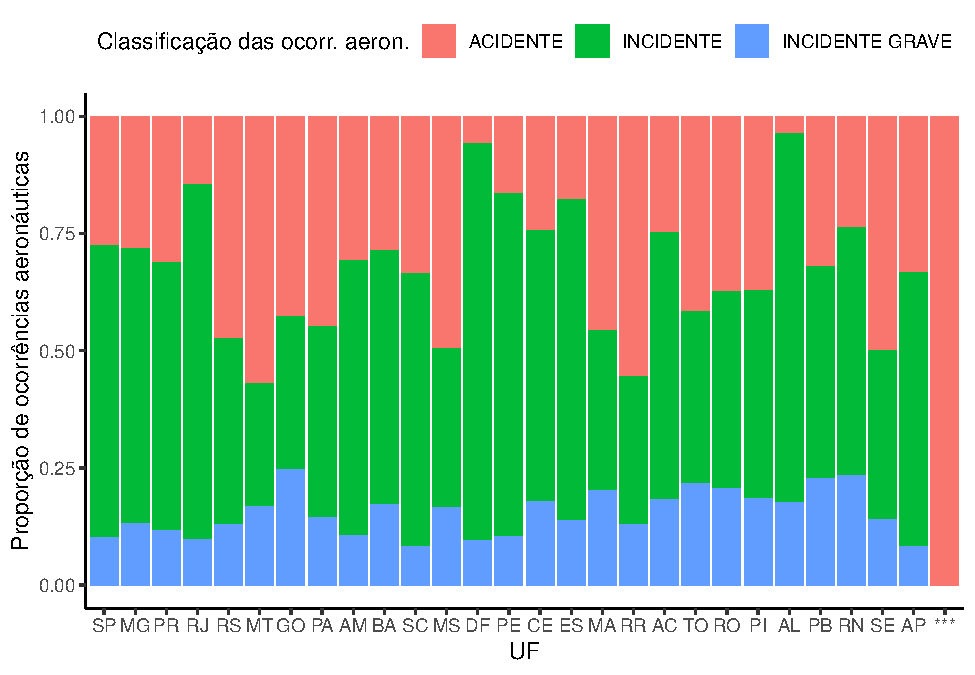
\includegraphics{4.Relatorio/pdf/index_files/figure-latex/unnamed-chunk-32-1} \end{center}

\begin{quote}
Naturalmente, pelo fato de existir maior movimentação de aviões em
estados de alta atividade econômica, esses mesmos têm as maiores
quantidades de ocorrências. Porém, são os estados de
MT(\textasciitilde56.9\%), RR(\textasciitilde55.6\%), e
SE(\textasciitilde50\%) que têm as maiores proporções de acidentes.
\end{quote}

\hypertarget{q4-ocorrem-mais-acidentes-na-sauxedda-da-pista}{%
\subsection{Q4 -- Ocorrem mais acidentes na saída da
pista?}\label{q4-ocorrem-mais-acidentes-na-sauxedda-da-pista}}

\begin{Shaded}
\begin{Highlighting}[]
\NormalTok{p\_ocor\_saida\_pista }\OtherTok{\textless{}{-}} \FunctionTok{calcula\_tab\_frequencia\_dplyr}\NormalTok{(}
    \AttributeTok{tabela\_de\_entrada =}\NormalTok{ ocorrencia,}
    \AttributeTok{nome\_variavel =} \StringTok{\textasciigrave{}}\AttributeTok{ocorrencia\_saida\_pista}\StringTok{\textasciigrave{}}
\NormalTok{)}

\ControlFlowTok{if}\NormalTok{ (kn}\SpecialCharTok{$}\FunctionTok{is\_html\_output}\NormalTok{()) \{}
\NormalTok{    p\_ocor\_saida\_pista}
\NormalTok{\} }\ControlFlowTok{else}\NormalTok{ \{}
\NormalTok{    p\_ocor\_saida\_pista }\SpecialCharTok{\%\textgreater{}\%}\NormalTok{ kn}\SpecialCharTok{$}\FunctionTok{kable}\NormalTok{()}
\NormalTok{\}}
\end{Highlighting}
\end{Shaded}

\begin{longtable}[]{@{}
  >{\raggedright\arraybackslash}p{(\columnwidth - 8\tabcolsep) * \real{0.1233}}
  >{\raggedleft\arraybackslash}p{(\columnwidth - 8\tabcolsep) * \real{0.1370}}
  >{\raggedleft\arraybackslash}p{(\columnwidth - 8\tabcolsep) * \real{0.1507}}
  >{\raggedleft\arraybackslash}p{(\columnwidth - 8\tabcolsep) * \real{0.2877}}
  >{\raggedleft\arraybackslash}p{(\columnwidth - 8\tabcolsep) * \real{0.3014}}@{}}
\toprule
\begin{minipage}[b]{\linewidth}\raggedright
Category
\end{minipage} & \begin{minipage}[b]{\linewidth}\raggedleft
Frequency
\end{minipage} & \begin{minipage}[b]{\linewidth}\raggedleft
Percentage
\end{minipage} & \begin{minipage}[b]{\linewidth}\raggedleft
Cumulative.Frequency
\end{minipage} & \begin{minipage}[b]{\linewidth}\raggedleft
Cumulative.Percentage
\end{minipage} \\
\midrule
\endhead
NÃO & 4684 & 90.652216 & 4684 & 90.65222 \\
SIM & 483 & 9.347784 & 5167 & 100.00000 \\
\bottomrule
\end{longtable}

\begin{Shaded}
\begin{Highlighting}[]
\DocumentationTok{\#\#\#\#\#\#\#\#\#\#\#\#\#\#\#\#\#\#\#\#\#\#\#\#\#\#\#\#\#\#\#\#\#\#\#\#\#\#\#\#\#\#\#\#\#\#\#\#\#\#\#\#\#\#\#\#\#\#\#\#\#\#\#\#\#\#\#\# Cria gráfico}

\CommentTok{\#source(\textquotesingle{}funcoes\_auxiliares/funcoes\_analiseunivariada.R\textquotesingle{},encoding="UTF{-}8")}
\NormalTok{ggplot2\_p\_ocor\_saida\_pista }\OtherTok{\textless{}{-}} \FunctionTok{grafico\_tab\_frequencia}\NormalTok{(}
    \AttributeTok{table\_count\_prop =}\NormalTok{ p\_ocor\_saida\_pista,}
    \AttributeTok{nome\_variavel =} \StringTok{"Category"}\NormalTok{,}
    \AttributeTok{cor\_grafico =} \StringTok{"\#77C6D9"}\NormalTok{,}
    \AttributeTok{hjust\_e =} \SpecialCharTok{{-}}\FloatTok{0.17}\NormalTok{,}
    \AttributeTok{hjust\_d =} \FloatTok{0.15}\NormalTok{,}
    \AttributeTok{size =} \FloatTok{4.5}\NormalTok{,}
    \AttributeTok{tx1 =} \FloatTok{0.05}\NormalTok{,}
    \AttributeTok{tx2 =} \DecValTok{1}\NormalTok{,}
    \AttributeTok{xlab =} \StringTok{"Ocorrências aeronáuticas na saída de pista"}\NormalTok{,}
    \AttributeTok{ylab =} \StringTok{"N° de ocorrências aeronáuticas"}
\NormalTok{)}

\DocumentationTok{\#\#\#\#\#\#\#\#\#\#\#\#\#\#\#\#\#\#\#\#\#\#\#\#\#\#\#\#\#\#\#\#\#\#\#\#\#\#\#\#\#\#\#\#\#\#\#\#\#\#\#\#\#\#\#\#\#\#\#\#\#\#\#\#\#\#\#\# Salva gráfico}

\CommentTok{\#source(\textquotesingle{}funcoes\_auxiliares/salva\_grafico.R\textquotesingle{}, encoding = "UTF{-}8")}
\FunctionTok{salva\_grafico}\NormalTok{(}\AttributeTok{ggplot2\_grafico =}\NormalTok{ ggplot2\_p\_ocor\_saida\_pista)}

\DocumentationTok{\#\#\#\#\#\#\#\#\#\#\#\#\#\#\#\#\#\#\#\#\#\#\#\#\#\#\#\#\#\#\#\#\#\#\#\#\#\#\#\#\#\#\#\#\#\#\#\#\#\#\#\#\#\#\#\#\#\#\#\#\#\#\#\#\#\#\#\# Leitura gráfico}

\CommentTok{\#source(\textquotesingle{}funcoes\_auxiliares/leitura\_grafico.R\textquotesingle{}, encoding = "UTF{-}8")}
\FunctionTok{leitura\_grafico}\NormalTok{(}\AttributeTok{ggplot2\_grafico =}\NormalTok{ ggplot2\_p\_ocor\_saida\_pista)}
\end{Highlighting}
\end{Shaded}

\begin{center}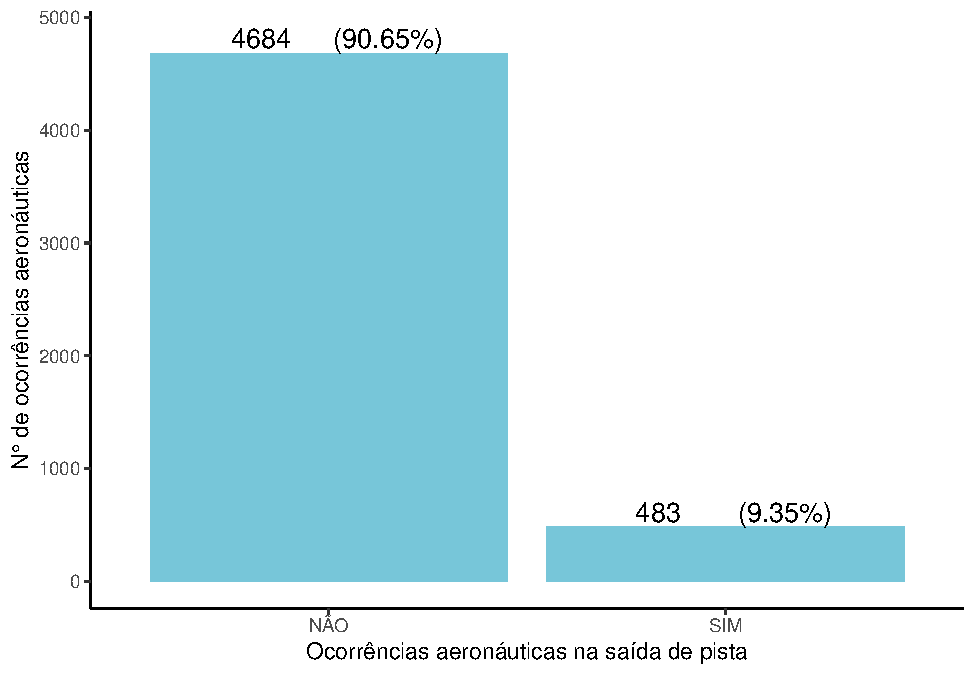
\includegraphics{4.Relatorio/pdf/index_files/figure-latex/unnamed-chunk-35-1} \end{center}

\begin{Shaded}
\begin{Highlighting}[]
\NormalTok{p\_ocor\_saida\_pista\_classif }\OtherTok{\textless{}{-}} \FunctionTok{calcula\_tab\_frequencia\_bivariada\_dplyr}\NormalTok{(ocorrencia,}
                                                             \StringTok{\textasciigrave{}}\AttributeTok{ocorrencia\_saida\_pista}\StringTok{\textasciigrave{}}\NormalTok{,}
                                                             \StringTok{\textasciigrave{}}\AttributeTok{ocorrencia\_classificacao}\StringTok{\textasciigrave{}}\NormalTok{)}
\end{Highlighting}
\end{Shaded}

\begin{verbatim}
## `summarise()` has grouped output by 'ocorrencia_saida_pista'. You can override using the `.groups` argument.
\end{verbatim}

\begin{Shaded}
\begin{Highlighting}[]
\NormalTok{p\_ocor\_saida\_pista\_classif}\SpecialCharTok{$}\StringTok{\textasciigrave{}}\AttributeTok{Percentage}\StringTok{\textasciigrave{}} \OtherTok{\textless{}{-}} \FunctionTok{round}\NormalTok{(p\_ocor\_saida\_pista\_classif}\SpecialCharTok{$}\StringTok{\textasciigrave{}}\AttributeTok{Percentage}\StringTok{\textasciigrave{}}\NormalTok{,}\DecValTok{1}\NormalTok{)}

\ControlFlowTok{if}\NormalTok{ (kn}\SpecialCharTok{$}\FunctionTok{is\_html\_output}\NormalTok{()) \{}
\NormalTok{    p\_ocor\_saida\_pista\_classif}
\NormalTok{\} }\ControlFlowTok{else}\NormalTok{ \{}
\NormalTok{    p\_ocor\_saida\_pista\_classif }\SpecialCharTok{\%\textgreater{}\%}\NormalTok{ kn}\SpecialCharTok{$}\FunctionTok{kable}\NormalTok{()}
\NormalTok{\}}
\end{Highlighting}
\end{Shaded}

\begin{longtable}[]{@{}
  >{\raggedright\arraybackslash}p{(\columnwidth - 8\tabcolsep) * \real{0.2771}}
  >{\raggedright\arraybackslash}p{(\columnwidth - 8\tabcolsep) * \real{0.3012}}
  >{\raggedleft\arraybackslash}p{(\columnwidth - 8\tabcolsep) * \real{0.1205}}
  >{\raggedleft\arraybackslash}p{(\columnwidth - 8\tabcolsep) * \real{0.1687}}
  >{\raggedleft\arraybackslash}p{(\columnwidth - 8\tabcolsep) * \real{0.1325}}@{}}
\toprule
\begin{minipage}[b]{\linewidth}\raggedright
ocorrencia\_saida\_pista
\end{minipage} & \begin{minipage}[b]{\linewidth}\raggedright
ocorrencia\_classificacao
\end{minipage} & \begin{minipage}[b]{\linewidth}\raggedleft
Frequency
\end{minipage} & \begin{minipage}[b]{\linewidth}\raggedleft
sum\_Frequency
\end{minipage} & \begin{minipage}[b]{\linewidth}\raggedleft
Percentage
\end{minipage} \\
\midrule
\endhead
NÃO & INCIDENTE GRAVE & 500 & 4684 & 10.7 \\
NÃO & INCIDENTE & 2767 & 4684 & 59.1 \\
NÃO & ACIDENTE & 1417 & 4684 & 30.3 \\
SIM & INCIDENTE GRAVE & 191 & 483 & 39.5 \\
SIM & ACIDENTE & 250 & 483 & 51.8 \\
SIM & INCIDENTE & 42 & 483 & 8.7 \\
\bottomrule
\end{longtable}

\begin{Shaded}
\begin{Highlighting}[]
\NormalTok{ggplot2\_ocor\_saida\_pista\_classif1 }\OtherTok{\textless{}{-}} \FunctionTok{grafico\_tab\_frequencia\_bivariada2}\NormalTok{(}
\NormalTok{    p\_ocor\_saida\_pista\_classif,}
    \StringTok{"ocorrencia\_classificacao"}\NormalTok{,}
    \StringTok{"ocorrencia\_saida\_pista"}\NormalTok{,}
    \AttributeTok{tx1 =} \FloatTok{0.3}\NormalTok{,}
    \AttributeTok{tx2 =} \FloatTok{1.3}\NormalTok{,}
    \AttributeTok{size =} \DecValTok{4}\NormalTok{,}
    \AttributeTok{legend =} \ConstantTok{TRUE}
\NormalTok{) }\SpecialCharTok{+}\NormalTok{ gg}\SpecialCharTok{$}\FunctionTok{scale\_fill\_discrete}\NormalTok{(}\AttributeTok{name =} \StringTok{"Classificação das ocorr. aeron."}\NormalTok{) }\SpecialCharTok{+}
\NormalTok{    gg}\SpecialCharTok{$}\FunctionTok{theme}\NormalTok{(}\AttributeTok{legend.position=}\StringTok{"top"}\NormalTok{) }\SpecialCharTok{+} 
\NormalTok{    gg}\SpecialCharTok{$}\FunctionTok{ylab}\NormalTok{(}\StringTok{\textquotesingle{}N° de ocorrências aeronáuticas\textquotesingle{}}\NormalTok{) }\SpecialCharTok{+}
\NormalTok{    gg}\SpecialCharTok{$}\FunctionTok{xlab}\NormalTok{(}\StringTok{\textquotesingle{}Ocorrências aeronáuticas na saída de pista\textquotesingle{}}\NormalTok{)}
\end{Highlighting}
\end{Shaded}

\begin{verbatim}
## [1] "Para retirar as porcentagens, use size = 0!"
\end{verbatim}

\begin{Shaded}
\begin{Highlighting}[]
\DocumentationTok{\#\#\#\#\#\#\#\#\#\#\#\#\#\#\#\#\#\#\#\#\#\#\#\#\#\#\#\#\#\#\#\#\#\#\#\#\#\#\#\#\#\#\#\#\#\#\#\#\#\#\#\#\#\#\#\#\#\#\#\#\#\#\#\#\#\#\#\# Salva gráfico}

\CommentTok{\#source(\textquotesingle{}funcoes\_auxiliares/salva\_grafico.R\textquotesingle{}, encoding = "UTF{-}8")}
\FunctionTok{salva\_grafico}\NormalTok{(}\AttributeTok{ggplot2\_grafico =}\NormalTok{ ggplot2\_ocor\_saida\_pista\_classif1)}

\DocumentationTok{\#\#\#\#\#\#\#\#\#\#\#\#\#\#\#\#\#\#\#\#\#\#\#\#\#\#\#\#\#\#\#\#\#\#\#\#\#\#\#\#\#\#\#\#\#\#\#\#\#\#\#\#\#\#\#\#\#\#\#\#\#\#\#\#\#\#\#\# Leitura gráfico}

\CommentTok{\#source(\textquotesingle{}funcoes\_auxiliares/leitura\_grafico.R\textquotesingle{}, encoding = "UTF{-}8")}
\FunctionTok{leitura\_grafico}\NormalTok{(}\AttributeTok{ggplot2\_grafico =}\NormalTok{ ggplot2\_ocor\_saida\_pista\_classif1)}
\end{Highlighting}
\end{Shaded}

\begin{center}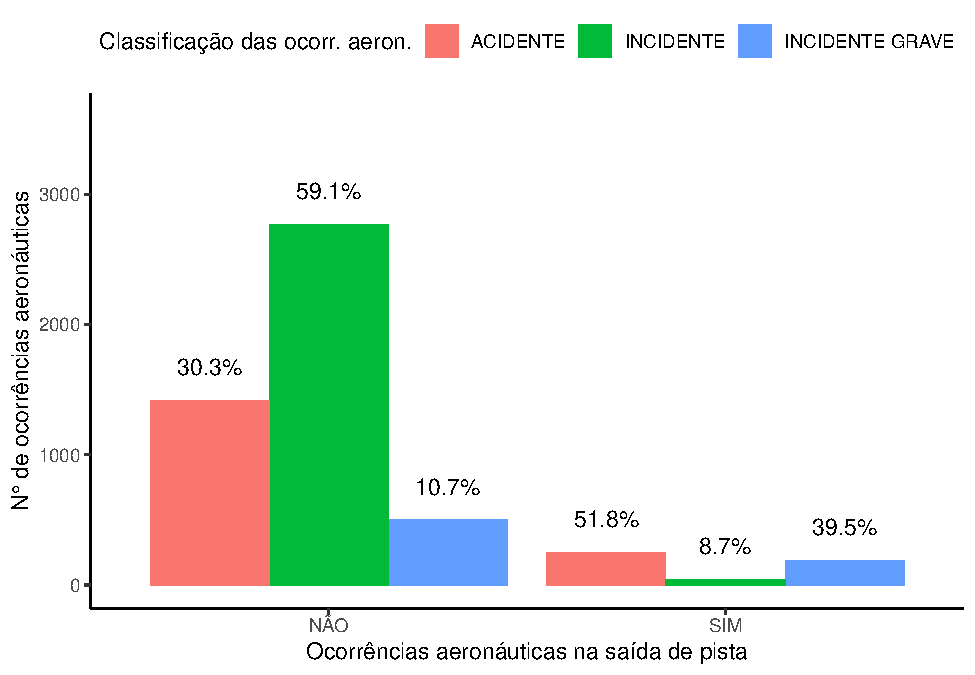
\includegraphics{4.Relatorio/pdf/index_files/figure-latex/unnamed-chunk-37-1} \end{center}

\begin{Shaded}
\begin{Highlighting}[]
\NormalTok{ggplot2\_ocor\_saida\_pista\_classif2 }\OtherTok{\textless{}{-}} \FunctionTok{grafico\_tab\_frequencia\_bivariada3}\NormalTok{(}
\NormalTok{    p\_ocor\_saida\_pista\_classif,}
    \StringTok{"ocorrencia\_classificacao"}\NormalTok{,}
    \StringTok{"ocorrencia\_saida\_pista"}\NormalTok{,}
    \AttributeTok{size =} \DecValTok{5}\NormalTok{,}
    \AttributeTok{tx1 =} \FloatTok{0.025}\NormalTok{,}
    \AttributeTok{tx2 =} \FloatTok{0.00025}\NormalTok{,}
    \AttributeTok{legend=}\ConstantTok{FALSE}
\NormalTok{) }\SpecialCharTok{+}\NormalTok{ gg}\SpecialCharTok{$}\FunctionTok{scale\_fill\_discrete}\NormalTok{(}\AttributeTok{name =} \StringTok{"Classificação das ocorr. aeron."}\NormalTok{) }\SpecialCharTok{+}
\NormalTok{    gg}\SpecialCharTok{$}\FunctionTok{theme}\NormalTok{(}\AttributeTok{legend.position=}\StringTok{"top"}\NormalTok{) }\SpecialCharTok{+} 
\NormalTok{    gg}\SpecialCharTok{$}\FunctionTok{ylab}\NormalTok{(}\StringTok{\textquotesingle{}Proporção de ocorrências aeronáuticas\textquotesingle{}}\NormalTok{) }\SpecialCharTok{+}
\NormalTok{    gg}\SpecialCharTok{$}\FunctionTok{xlab}\NormalTok{(}\StringTok{\textquotesingle{}Ocorrências aeronáuticas na saída de pista\textquotesingle{}}\NormalTok{)}

\DocumentationTok{\#\#\#\#\#\#\#\#\#\#\#\#\#\#\#\#\#\#\#\#\#\#\#\#\#\#\#\#\#\#\#\#\#\#\#\#\#\#\#\#\#\#\#\#\#\#\#\#\#\#\#\#\#\#\#\#\#\#\#\#\#\#\#\#\#\#\#\# Salva gráfico}

\CommentTok{\#source(\textquotesingle{}funcoes\_auxiliares/salva\_grafico.R\textquotesingle{}, encoding = "UTF{-}8")}
\FunctionTok{salva\_grafico}\NormalTok{(}\AttributeTok{ggplot2\_grafico =}\NormalTok{ ggplot2\_ocor\_saida\_pista\_classif2, }\AttributeTok{subir\_eixo\_y =}\NormalTok{ T)}

\DocumentationTok{\#\#\#\#\#\#\#\#\#\#\#\#\#\#\#\#\#\#\#\#\#\#\#\#\#\#\#\#\#\#\#\#\#\#\#\#\#\#\#\#\#\#\#\#\#\#\#\#\#\#\#\#\#\#\#\#\#\#\#\#\#\#\#\#\#\#\#\# Leitura gráfico}

\CommentTok{\#source(\textquotesingle{}funcoes\_auxiliares/leitura\_grafico.R\textquotesingle{}, encoding = "UTF{-}8")}
\FunctionTok{leitura\_grafico}\NormalTok{(}\AttributeTok{ggplot2\_grafico =}\NormalTok{ ggplot2\_ocor\_saida\_pista\_classif2)}
\end{Highlighting}
\end{Shaded}

\begin{center}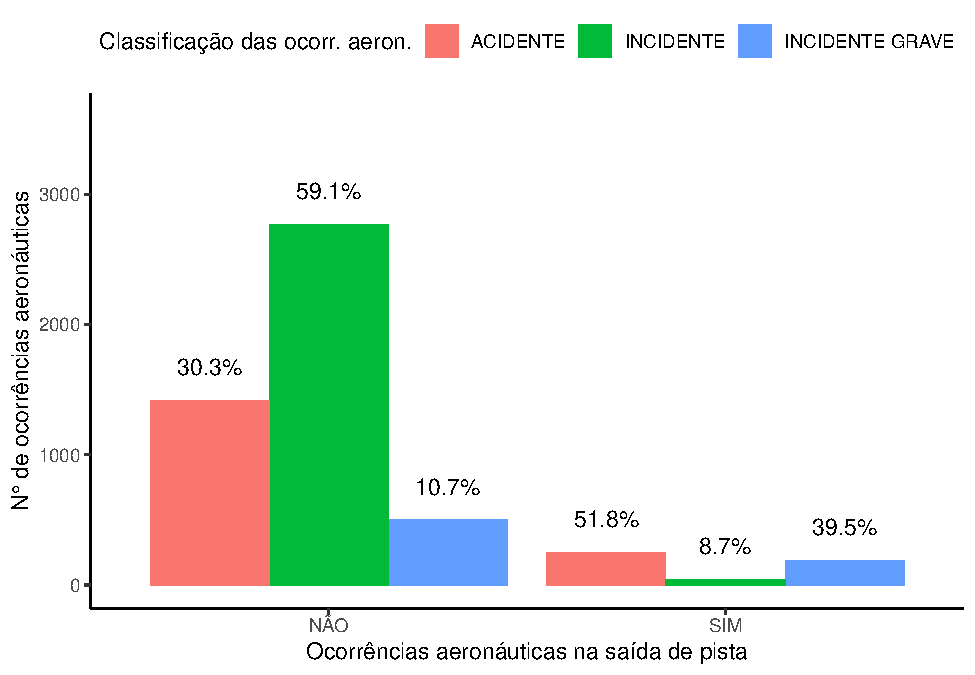
\includegraphics{4.Relatorio/pdf/index_files/figure-latex/unnamed-chunk-38-1} \end{center}

\begin{quote}
Não se observa uma quantidade maior de ocorrências nas saídas de pista,
porém a proporção de ocorrências classificadas como acidentes é maior
quando se tem uma ocorrência na saída de pista (51.8\% \textgreater{}
30.3\%).
\end{quote}

\hypertarget{q5-quais-suxe3o-os-tipos-de-ocorruxeancia-associadas-com-maior-proporuxe7uxe3o-de-acidentes}{%
\subsection{Q5 -- Quais são os tipos de ocorrência associadas com maior
proporção de
acidentes?}\label{q5-quais-suxe3o-os-tipos-de-ocorruxeancia-associadas-com-maior-proporuxe7uxe3o-de-acidentes}}

\begin{Shaded}
\begin{Highlighting}[]
\NormalTok{ocorrenciatipo }\OtherTok{\textless{}{-}}\NormalTok{ dp}\SpecialCharTok{$}\FunctionTok{tbl}\NormalTok{(con, }\StringTok{"ocorrenciatipo"}\NormalTok{)}
\NormalTok{ocorrencia\_ocorrenciatipo }\OtherTok{\textless{}{-}}\NormalTok{ dp}\SpecialCharTok{$}\FunctionTok{tbl}\NormalTok{(con, }\StringTok{"ocorrencia\_ocorrenciatipo"}\NormalTok{)}
\end{Highlighting}
\end{Shaded}

\begin{Shaded}
\begin{Highlighting}[]
\NormalTok{ocorrencia\_ocorrenciatipo\_aux }\OtherTok{\textless{}{-}}
\NormalTok{    dplyr}\SpecialCharTok{::}\FunctionTok{left\_join}\NormalTok{(}\AttributeTok{x =}\NormalTok{ ocorrencia\_ocorrenciatipo,}
                     \AttributeTok{y =}\NormalTok{ ocorrenciatipo,}
                     \AttributeTok{by =} \StringTok{\textquotesingle{}codigo\_ocorrencia\_tipo\textquotesingle{}}\NormalTok{) }\SpecialCharTok{\%\textgreater{}\%}
\NormalTok{    dplyr}\SpecialCharTok{::}\FunctionTok{left\_join}\NormalTok{(}
        \AttributeTok{x =}\NormalTok{ .,}
        \AttributeTok{y =}\NormalTok{ (}
\NormalTok{            ocorrencia\_ocorrenciatipo }\SpecialCharTok{\%\textgreater{}\%}
\NormalTok{                dp}\SpecialCharTok{$}\FunctionTok{select}\NormalTok{(codigo\_ocorrencia) }\SpecialCharTok{\%\textgreater{}\%}
\NormalTok{                dp}\SpecialCharTok{$}\FunctionTok{group\_by}\NormalTok{(codigo\_ocorrencia) }\SpecialCharTok{\%\textgreater{}\%}
\NormalTok{                dp}\SpecialCharTok{$}\FunctionTok{summarise}\NormalTok{(}\AttributeTok{codigo\_ocorrencia\_count =}\NormalTok{ dplyr}\SpecialCharTok{::}\FunctionTok{n}\NormalTok{())}
\NormalTok{        ),}
        \AttributeTok{by =} \StringTok{\textquotesingle{}codigo\_ocorrencia\textquotesingle{}}
\NormalTok{    ) }\SpecialCharTok{\%\textgreater{}\%} 
\NormalTok{    dplyr}\SpecialCharTok{::}\FunctionTok{mutate}\NormalTok{(}\AttributeTok{ocorrencia\_tipo\_new =} \FunctionTok{ifelse}\NormalTok{(codigo\_ocorrencia\_count}\SpecialCharTok{==}\DecValTok{1}\NormalTok{,}
\NormalTok{                                               ocorrencia\_tipo,}
\NormalTok{                                                (}\FunctionTok{ifelse}\NormalTok{(codigo\_ocorrencia\_count}\SpecialCharTok{==}\DecValTok{2}\NormalTok{,}
                                                        \StringTok{\textquotesingle{}2 TIPOS DE OCORRÊNCIA\textquotesingle{}}\NormalTok{,}
\NormalTok{                                                        (}\FunctionTok{ifelse}\NormalTok{(codigo\_ocorrencia\_count}\SpecialCharTok{==}\DecValTok{3}\NormalTok{,}
                                                                \StringTok{\textquotesingle{}3 TIPOS DE OCORRÊNCIA\textquotesingle{}}\NormalTok{,}
                                                                \StringTok{\textquotesingle{}NA\textquotesingle{}}\NormalTok{)) )))) }\SpecialCharTok{\%\textgreater{}\%} 
\NormalTok{    dplyr}\SpecialCharTok{::}\FunctionTok{select}\NormalTok{(codigo\_ocorrencia, codigo\_ocorrencia\_tipo, ocorrencia\_tipo, ocorrencia\_tipo\_new) }\SpecialCharTok{\%\textgreater{}\%} 
    \FunctionTok{as.data.frame}\NormalTok{()}

\NormalTok{ocorrencia\_ocorrenciatipo\_aux1}\FloatTok{.5} \OtherTok{\textless{}{-}}\NormalTok{ocorrencia\_ocorrenciatipo\_aux }\SpecialCharTok{\%\textgreater{}\%}\NormalTok{ dplyr}\SpecialCharTok{::}\FunctionTok{select}\NormalTok{(codigo\_ocorrencia,}
\NormalTok{                                                        ocorrencia\_tipo\_new) }\SpecialCharTok{\%\textgreater{}\%} 
\NormalTok{            dplyr}\SpecialCharTok{::}\FunctionTok{distinct}\NormalTok{() }\SpecialCharTok{\%\textgreater{}\%} \FunctionTok{as.data.frame}\NormalTok{()}

\NormalTok{ocorrencia\_ocorrenciatipo\_aux2 }\OtherTok{\textless{}{-}}\NormalTok{ ocorrencia }\SpecialCharTok{\%\textgreater{}\%}
    \FunctionTok{as.data.frame}\NormalTok{() }\SpecialCharTok{\%\textgreater{}\%} 
\NormalTok{    dplyr}\SpecialCharTok{::}\FunctionTok{select}\NormalTok{(codigo\_ocorrencia, ocorrencia\_classificacao) }\SpecialCharTok{\%\textgreater{}\%}
\NormalTok{    dplyr}\SpecialCharTok{::}\FunctionTok{left\_join}\NormalTok{(}
        \AttributeTok{x =}\NormalTok{ .,}
        \AttributeTok{y =}\NormalTok{ ocorrencia\_ocorrenciatipo\_aux1}\FloatTok{.5}\NormalTok{,}
        \AttributeTok{by =} \StringTok{\textquotesingle{}codigo\_ocorrencia\textquotesingle{}}
\NormalTok{    )}
\end{Highlighting}
\end{Shaded}

\begin{Shaded}
\begin{Highlighting}[]
\NormalTok{p\_ocor\_ocorrencia\_tipo\_new }\OtherTok{\textless{}{-}} \FunctionTok{calcula\_tab\_frequencia\_dplyr}\NormalTok{(}
    \AttributeTok{tabela\_de\_entrada =}\NormalTok{ ocorrencia\_ocorrenciatipo\_aux2,}
    \AttributeTok{nome\_variavel =} \StringTok{\textasciigrave{}}\AttributeTok{ocorrencia\_tipo\_new}\StringTok{\textasciigrave{}}
\NormalTok{)}

\NormalTok{p\_ocor\_ocorrencia\_tipo\_new }\OtherTok{\textless{}{-}}\NormalTok{ p\_ocor\_ocorrencia\_tipo\_new }\SpecialCharTok{\%\textgreater{}\%}\NormalTok{ dp}\SpecialCharTok{$}\FunctionTok{arrange}\NormalTok{(dp}\SpecialCharTok{$}\FunctionTok{desc}\NormalTok{(Frequency))}
\NormalTok{p\_ocor\_ocorrencia\_tipo\_new}\SpecialCharTok{$}\StringTok{\textasciigrave{}}\AttributeTok{Percentage}\StringTok{\textasciigrave{}} \OtherTok{\textless{}{-}} \FunctionTok{round}\NormalTok{(p\_ocor\_ocorrencia\_tipo\_new}\SpecialCharTok{$}\StringTok{\textasciigrave{}}\AttributeTok{Percentage}\StringTok{\textasciigrave{}}\NormalTok{,}\DecValTok{1}\NormalTok{)}
\NormalTok{p\_ocor\_ocorrencia\_tipo\_new[[}\StringTok{\textquotesingle{}Category\textquotesingle{}}\NormalTok{]] }\OtherTok{\textless{}{-}} \FunctionTok{factor}\NormalTok{(p\_ocor\_ocorrencia\_tipo\_new[[}\StringTok{\textquotesingle{}Category\textquotesingle{}}\NormalTok{]],}
                                                   \AttributeTok{levels=}\FunctionTok{rev}\NormalTok{(p\_ocor\_ocorrencia\_tipo\_new[[}\StringTok{\textquotesingle{}Category\textquotesingle{}}\NormalTok{]]))}

\ControlFlowTok{if}\NormalTok{ (kn}\SpecialCharTok{$}\FunctionTok{is\_html\_output}\NormalTok{()) \{}
\NormalTok{    p\_ocor\_ocorrencia\_tipo\_new}
\NormalTok{\} }\ControlFlowTok{else}\NormalTok{ \{}
\NormalTok{    p\_ocor\_ocorrencia\_tipo\_new }\SpecialCharTok{\%\textgreater{}\%}\NormalTok{ kn}\SpecialCharTok{$}\FunctionTok{kable}\NormalTok{()}
\NormalTok{\}}
\end{Highlighting}
\end{Shaded}

\begin{longtable}[]{@{}
  >{\raggedright\arraybackslash}p{(\columnwidth - 8\tabcolsep) * \real{0.5924}}
  >{\raggedleft\arraybackslash}p{(\columnwidth - 8\tabcolsep) * \real{0.0637}}
  >{\raggedleft\arraybackslash}p{(\columnwidth - 8\tabcolsep) * \real{0.0701}}
  >{\raggedleft\arraybackslash}p{(\columnwidth - 8\tabcolsep) * \real{0.1338}}
  >{\raggedleft\arraybackslash}p{(\columnwidth - 8\tabcolsep) * \real{0.1401}}@{}}
\toprule
\begin{minipage}[b]{\linewidth}\raggedright
Category
\end{minipage} & \begin{minipage}[b]{\linewidth}\raggedleft
Frequency
\end{minipage} & \begin{minipage}[b]{\linewidth}\raggedleft
Percentage
\end{minipage} & \begin{minipage}[b]{\linewidth}\raggedleft
Cumulative.Frequency
\end{minipage} & \begin{minipage}[b]{\linewidth}\raggedleft
Cumulative.Percentage
\end{minipage} \\
\midrule
\endhead
FALHA DO MOTOR EM VOO & 655 & 12.7 & 2667 & 51.6160248 \\
FALHA OU MAU FUNCIONAMENTO DE SISTEMA / COMPONENTE & 589 & 11.4 & 3288 &
63.6346042 \\
ESTOURO DE PNEU & 571 & 11.1 & 1896 & 36.6944068 \\
PERDA DE CONTROLE NO SOLO & 313 & 6.1 & 4624 & 89.4910006 \\
COM TREM DE POUSO & 295 & 5.7 & 1246 & 24.1145733 \\
PERDA DE CONTROLE EM VOO & 293 & 5.7 & 4311 & 83.4333269 \\
OUTROS & 244 & 4.7 & 3859 & 74.6855042 \\
COLISÃO COM AVE & 198 & 3.8 & 512 & 9.9090381 \\
COLISÃO COM OBSTÁCULO DURANTE A DECOLAGEM E POUSO & 168 & 3.3 & 702 &
13.5862202 \\
2 TIPOS DE OCORRÊNCIA & 166 & 3.2 & 167 & 3.2320495 \\
INDETERMINADO & 125 & 2.4 & 3527 & 68.2601123 \\
POUSO BRUSCO & 90 & 1.7 & 4731 & 91.5618347 \\
COLISÃO COM OBSTÁCULOS NO SOLO & 86 & 1.7 & 788 & 15.2506290 \\
PANE SECA & 86 & 1.7 & 3945 & 76.3499129 \\
POUSO EM LOCAL NÃO PREVISTO & 86 & 1.7 & 4817 & 93.2262435 \\
CAUSADO POR FENÔMENO METEOROLÓGICO EM VOO & 82 & 1.6 & 288 &
5.5738339 \\
POUSO SEM TREM & 77 & 1.5 & 4947 & 95.7422102 \\
TRÁFEGO AÉREO & 77 & 1.5 & 5066 & 98.0452874 \\
EXCURSÃO DE PISTA & 76 & 1.5 & 1972 & 38.1652797 \\
OPERAÇÃO A BAIXA ALTITUDE & 71 & 1.4 & 3606 & 69.7890459 \\
COM PARA-BRISAS / JANELA / PORTA & 67 & 1.3 & 933 & 18.0568996 \\
POUSO LONGO & 53 & 1.0 & 4870 & 94.2519837 \\
VAZAMENTO DE OUTROS FLUIDOS & 48 & 0.9 & 5136 & 99.4000387 \\
PERDA DE COMPONENTE EM VOO & 46 & 0.9 & 3995 & 77.3175924 \\
DESCOMPRESSÃO NÃO INTENCIONAL / EXPLOSIVA & 40 & 0.8 & 1320 &
25.5467389 \\
F.O.D. & 39 & 0.8 & 2012 & 38.9394233 \\
VOO CONTROLADO CONTRA O TERRENO & 31 & 0.6 & 5167 & 100.0000000 \\
FALHA OU MAU FUNCIONAMENTO DO MOTOR & 29 & 0.6 & 3317 & 64.1958583 \\
FUMAÇA NA CABINE & 25 & 0.5 & 3375 & 65.3183666 \\
FALHA DO MOTOR NO SOLO & 24 & 0.5 & 2691 & 52.0805109 \\
COLISÃO COM FAUNA & 22 & 0.4 & 534 & 10.3348171 \\
COM COMANDOS DE VOO & 22 & 0.4 & 839 & 16.2376621 \\
PERDA DE COMPONENTE NO SOLO & 21 & 0.4 & 4016 & 77.7240178 \\
COM HÉLICE & 20 & 0.4 & 859 & 16.6247339 \\
INCURSÃO EM PISTA & 20 & 0.4 & 3402 & 65.8409135 \\
FOGO NO SOLO & 18 & 0.3 & 3341 & 64.6603445 \\
POUSO ANTES DA PISTA & 15 & 0.3 & 4640 & 89.8006580 \\
ALARME FALSO DE FOGO OU DE SUPERAQUECIMENTO & 14 & 0.3 & 206 &
3.9868396 \\
SOPRO DE REATOR & 14 & 0.3 & 4972 & 96.2260499 \\
SUPERAQUECIMENTO & 14 & 0.3 & 4989 & 96.5550610 \\
VAZAMENTO DE COMBUSTÍVEL & 14 & 0.3 & 5088 & 98.4710664 \\
COLISÃO COM AERONAVE NO SOLO & 13 & 0.3 & 314 & 6.0770273 \\
AERONAVE ATINGIDA POR OBJETO & 12 & 0.2 & 192 & 3.7158893 \\
CAUSADO POR FENÔMENO METEOROLÓGICO NO SOLO & 12 & 0.2 & 300 &
5.8060770 \\
COM ROTOR & 11 & 0.2 & 949 & 18.3665570 \\
COMBUSTÍVEL & 10 & 0.2 & 1256 & 24.3081092 \\
COLISÃO DE AERONAVES EM VOO & 9 & 0.2 & 797 & 15.4248113 \\
COLISÃO DE VEÍCULO COM AERONAVE & 9 & 0.2 & 806 & 15.5989936 \\
CONTATO ANORMAL COM A PISTAA & 9 & 0.2 & 1269 & 24.5597058 \\
OPERAÇÕES NO SOLO & 9 & 0.2 & 3615 & 69.9632282 \\
PROBLEMAS FISIOLÓGICOS & 9 & 0.2 & 4956 & 95.9163925 \\
FALHA ESTRUTURAL & 8 & 0.2 & 2699 & 52.2353397 \\
MANOBRA ABRUPTA & 8 & 0.2 & 3535 & 68.4149410 \\
TURBULÊNCIA & 8 & 0.2 & 5074 & 98.2001161 \\
3 TIPOS DE OCORRÊNCIA & 7 & 0.1 & 174 & 3.3675247 \\
COM CARGAS EXTERNAS & 7 & 0.1 & 817 & 15.8118831 \\
FOGO/FUMAÇA (SEM IMPACTO) & 7 & 0.1 & 3348 & 64.7958196 \\
AERÓDROMO & 6 & 0.1 & 180 & 3.4836462 \\
CORTE INVOLUNTÁRIO DO MOTOR & 6 & 0.1 & 1280 & 24.7725953 \\
FOGO EM VOO & 6 & 0.1 & 3323 & 64.3119799 \\
COM PESSOAL EM VOO & 5 & 0.1 & 938 & 18.1536675 \\
CORTANTE DE VENTO / TEMPESTADE & 5 & 0.1 & 1274 & 24.6564738 \\
DESORIENTAÇÃO ESPACIAL & 5 & 0.1 & 1325 & 25.6435069 \\
GERENCIAMENTO DE TRÁFEGO AÉREO (ATM) / SERVIÇO DE COMUNICAÇÃO NAVEGAÇÃO,
OU VIGILÂNCIA (CNS) & 5 & 0.1 & 3380 & 65.4151345 \\
COM LANÇAMENTO DE CARGA & 4 & 0.1 & 863 & 16.7021482 \\
CONTATO ANORMAL COM A PISTA & 4 & 0.1 & 1260 & 24.3855235 \\
PERDA DA CONSCIÊNCIA & 4 & 0.1 & 3949 & 76.4273273 \\
COM LANÇAMENTO DE PESSOAS & 3 & 0.1 & 866 & 16.7602090 \\
SOPRO DE ROTOR & 3 & 0.1 & 4975 & 96.2841107 \\
COLISÃO EM VOO COM OBSTÁCULO & 2 & 0.0 & 808 & 15.6377008 \\
COLISÃO NO SOLO & 2 & 0.0 & 810 & 15.6764080 \\
COM TRANSPORTE DE CARGA & 2 & 0.0 & 951 & 18.4052642 \\
FORMAÇÃO DE GELO & 2 & 0.0 & 3350 & 64.8345268 \\
PERDA DE CONDIÇÕES DE SUSTENTAÇÃO EM ROTA & 2 & 0.0 & 4018 &
77.7627250 \\
& 1 & 0.0 & 1 & 0.0193536 \\
CAUSADO POR RICOCHETE & 1 & 0.0 & 301 & 5.8254306 \\
EXPLOSÃO & 1 & 0.0 & 1973 & 38.1846332 \\
HIPÓXIA & 1 & 0.0 & 3381 & 65.4344881 \\
IMC NÃO INTENCIONAL & 1 & 0.0 & 3382 & 65.4538417 \\
PERDA DE SEPARAÇÃO / COLISÃO EM VOO & 1 & 0.0 & 4625 & 89.5103542 \\
POUSO AQUÉM/ALÉM DA PISTA & 1 & 0.0 & 4641 & 89.8200116 \\
REBOQUE DE PLANADOR & 1 & 0.0 & 4957 & 95.9357461 \\
RELACIONADO COM SECURITY & 1 & 0.0 & 4958 & 95.9550997 \\
\bottomrule
\end{longtable}

\begin{Shaded}
\begin{Highlighting}[]
\DocumentationTok{\#\#\#\#\#\#\#\#\#\#\#\#\#\#\#\#\#\#\#\#\#\#\#\#\#\#\#\#\#\#\#\#\#\#\#\#\#\#\#\#\#\#\#\#\#\#\#\#\#\#\#\#\#\#\#\#\#\#\#\#\#\#\#\#\#\#\#\# Cria gráfico}

\CommentTok{\#source(\textquotesingle{}funcoes\_auxiliares/funcoes\_analiseunivariada.R\textquotesingle{},encoding="UTF{-}8")}
\NormalTok{ggplot2\_p\_ocor\_ocorrencia\_tipo\_new }\OtherTok{\textless{}{-}} \FunctionTok{grafico\_tab\_frequencia2}\NormalTok{(}
    \AttributeTok{table\_count\_prop =}\NormalTok{ p\_ocor\_ocorrencia\_tipo\_new,}
    \AttributeTok{nome\_variavel =} \StringTok{\textquotesingle{}ocorrencia\_tipo\_new\textquotesingle{}}\NormalTok{,}
    \AttributeTok{cor\_grafico =} \StringTok{\textquotesingle{}\#77C6D9\textquotesingle{}}\NormalTok{,}
    \AttributeTok{size =} \DecValTok{5}\NormalTok{,}
    \AttributeTok{tx1 =} \FloatTok{1.5}\NormalTok{,}
    \AttributeTok{tx2 =} \FloatTok{1.2}
\NormalTok{)}

\NormalTok{ggplot2\_p\_ocor\_ocorrencia\_tipo\_new }\OtherTok{\textless{}{-}}\NormalTok{ ggplot2\_p\_ocor\_ocorrencia\_tipo\_new }\SpecialCharTok{+} 
\NormalTok{                                        gg}\SpecialCharTok{$}\FunctionTok{scale\_x\_discrete}\NormalTok{(}
                                        \AttributeTok{labels =} \ControlFlowTok{function}\NormalTok{(x) \{}
\NormalTok{                                              is\_long }\OtherTok{\textless{}{-}} \FunctionTok{nchar}\NormalTok{(x) }\SpecialCharTok{\textgreater{}} \DecValTok{25}
\NormalTok{                                              x[is\_long] }\OtherTok{\textless{}{-}} \FunctionTok{paste0}\NormalTok{(}\FunctionTok{substr}\NormalTok{(x[is\_long], }\DecValTok{1}\NormalTok{, }\DecValTok{25}\NormalTok{), }\StringTok{"."}\NormalTok{)}
\NormalTok{                                              x}
\NormalTok{                                            \}}
\NormalTok{                                          ) }\SpecialCharTok{+}
\NormalTok{    gg}\SpecialCharTok{$}\FunctionTok{coord\_flip}\NormalTok{(}\AttributeTok{xlim=}\FunctionTok{c}\NormalTok{(p\_ocor\_ocorrencia\_tipo\_new[[}\StringTok{\textquotesingle{}Category\textquotesingle{}}\NormalTok{]][}\DecValTok{1}\NormalTok{],}
\NormalTok{                         p\_ocor\_ocorrencia\_tipo\_new[[}\StringTok{\textquotesingle{}Category\textquotesingle{}}\NormalTok{]][}\DecValTok{6}\NormalTok{])) }\SpecialCharTok{+}
\NormalTok{    gg}\SpecialCharTok{$}\FunctionTok{xlab}\NormalTok{(}\StringTok{\textquotesingle{}Tipo de ocorr. aeron.\textquotesingle{}}\NormalTok{) }\SpecialCharTok{+}
\NormalTok{    gg}\SpecialCharTok{$}\FunctionTok{ylab}\NormalTok{(}\StringTok{\textquotesingle{}N° de ocorrências aeronáuticas\textquotesingle{}}\NormalTok{)}

\DocumentationTok{\#\#\#\#\#\#\#\#\#\#\#\#\#\#\#\#\#\#\#\#\#\#\#\#\#\#\#\#\#\#\#\#\#\#\#\#\#\#\#\#\#\#\#\#\#\#\#\#\#\#\#\#\#\#\#\#\#\#\#\#\#\#\#\#\#\#\#\# Salva gráfico}

\CommentTok{\#source(\textquotesingle{}funcoes\_auxiliares/salva\_grafico.R\textquotesingle{}, encoding = "UTF{-}8")}
\FunctionTok{salva\_grafico}\NormalTok{(}\AttributeTok{ggplot2\_grafico =}\NormalTok{ ggplot2\_p\_ocor\_ocorrencia\_tipo\_new)}

\DocumentationTok{\#\#\#\#\#\#\#\#\#\#\#\#\#\#\#\#\#\#\#\#\#\#\#\#\#\#\#\#\#\#\#\#\#\#\#\#\#\#\#\#\#\#\#\#\#\#\#\#\#\#\#\#\#\#\#\#\#\#\#\#\#\#\#\#\#\#\#\# Leitura gráfico}

\CommentTok{\#source(\textquotesingle{}funcoes\_auxiliares/leitura\_grafico.R\textquotesingle{}, encoding = "UTF{-}8")}
\FunctionTok{leitura\_grafico}\NormalTok{(}\AttributeTok{ggplot2\_grafico =}\NormalTok{ ggplot2\_p\_ocor\_ocorrencia\_tipo\_new)}
\end{Highlighting}
\end{Shaded}

\begin{center}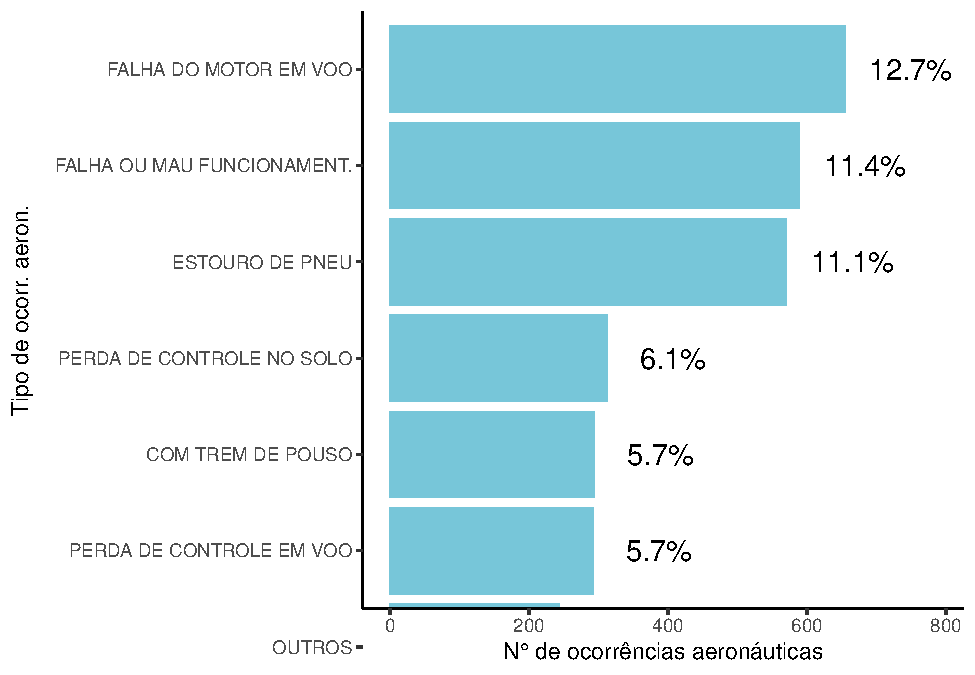
\includegraphics{4.Relatorio/pdf/index_files/figure-latex/unnamed-chunk-43-1} \end{center}

\begin{Shaded}
\begin{Highlighting}[]
\NormalTok{p\_ocor\_ocorrencia\_tipo\_new\_classif }\OtherTok{\textless{}{-}} \FunctionTok{calcula\_tab\_frequencia\_bivariada\_dplyr}\NormalTok{(ocorrencia\_ocorrenciatipo\_aux2,}
                                                             \StringTok{\textasciigrave{}}\AttributeTok{ocorrencia\_tipo\_new}\StringTok{\textasciigrave{}}\NormalTok{,}
                                                             \StringTok{\textasciigrave{}}\AttributeTok{ocorrencia\_classificacao}\StringTok{\textasciigrave{}}\NormalTok{)}
\end{Highlighting}
\end{Shaded}

\begin{verbatim}
## `summarise()` has grouped output by 'ocorrencia_tipo_new'. You can override using the `.groups` argument.
\end{verbatim}

\begin{Shaded}
\begin{Highlighting}[]
\NormalTok{p\_ocor\_ocorrencia\_tipo\_new\_classif }\OtherTok{\textless{}{-}}\NormalTok{ p\_ocor\_ocorrencia\_tipo\_new\_classif }\SpecialCharTok{\%\textgreater{}\%} 
\NormalTok{                    dplyr}\SpecialCharTok{::}\FunctionTok{arrange}\NormalTok{(}\FunctionTok{match}\NormalTok{(}\StringTok{\textasciigrave{}}\AttributeTok{ocorrencia\_tipo\_new}\StringTok{\textasciigrave{}}\NormalTok{, p\_ocor\_ocorrencia\_tipo\_new[[}\StringTok{\textquotesingle{}Category\textquotesingle{}}\NormalTok{]]))}
\NormalTok{p\_ocor\_ocorrencia\_tipo\_new\_classif}\SpecialCharTok{$}\StringTok{\textasciigrave{}}\AttributeTok{Percentage}\StringTok{\textasciigrave{}} \OtherTok{\textless{}{-}} \FunctionTok{round}\NormalTok{(p\_ocor\_ocorrencia\_tipo\_new\_classif}\SpecialCharTok{$}\StringTok{\textasciigrave{}}\AttributeTok{Percentage}\StringTok{\textasciigrave{}}\NormalTok{,}\DecValTok{1}\NormalTok{)}
\NormalTok{p\_ocor\_ocorrencia\_tipo\_new\_classif[[}\StringTok{\textquotesingle{}ocorrencia\_tipo\_new\textquotesingle{}}\NormalTok{]] }\OtherTok{\textless{}{-}}\NormalTok{ fc}\SpecialCharTok{$}\FunctionTok{fct\_rev}\NormalTok{(fc}\SpecialCharTok{$}\FunctionTok{fct\_inorder}\NormalTok{(}
\NormalTok{    p\_ocor\_ocorrencia\_tipo\_new\_classif[[}\StringTok{\textquotesingle{}ocorrencia\_tipo\_new\textquotesingle{}}\NormalTok{]])}
\NormalTok{    )}

\ControlFlowTok{if}\NormalTok{ (kn}\SpecialCharTok{$}\FunctionTok{is\_html\_output}\NormalTok{()) \{}
\NormalTok{    p\_ocor\_ocorrencia\_tipo\_new\_classif}
\NormalTok{\} }\ControlFlowTok{else}\NormalTok{ \{}
\NormalTok{    p\_ocor\_ocorrencia\_tipo\_new\_classif }\SpecialCharTok{\%\textgreater{}\%}\NormalTok{ kn}\SpecialCharTok{$}\FunctionTok{kable}\NormalTok{()}
\NormalTok{\}}
\end{Highlighting}
\end{Shaded}

\begin{longtable}[]{@{}
  >{\raggedright\arraybackslash}p{(\columnwidth - 8\tabcolsep) * \real{0.6078}}
  >{\raggedright\arraybackslash}p{(\columnwidth - 8\tabcolsep) * \real{0.1634}}
  >{\raggedleft\arraybackslash}p{(\columnwidth - 8\tabcolsep) * \real{0.0654}}
  >{\raggedleft\arraybackslash}p{(\columnwidth - 8\tabcolsep) * \real{0.0915}}
  >{\raggedleft\arraybackslash}p{(\columnwidth - 8\tabcolsep) * \real{0.0719}}@{}}
\toprule
\begin{minipage}[b]{\linewidth}\raggedright
ocorrencia\_tipo\_new
\end{minipage} & \begin{minipage}[b]{\linewidth}\raggedright
ocorrencia\_classificacao
\end{minipage} & \begin{minipage}[b]{\linewidth}\raggedleft
Frequency
\end{minipage} & \begin{minipage}[b]{\linewidth}\raggedleft
sum\_Frequency
\end{minipage} & \begin{minipage}[b]{\linewidth}\raggedleft
Percentage
\end{minipage} \\
\midrule
\endhead
FALHA DO MOTOR EM VOO & ACIDENTE & 332 & 655 & 50.7 \\
FALHA DO MOTOR EM VOO & INCIDENTE & 230 & 655 & 35.1 \\
FALHA DO MOTOR EM VOO & INCIDENTE GRAVE & 93 & 655 & 14.2 \\
FALHA OU MAU FUNCIONAMENTO DE SISTEMA / COMPONENTE & ACIDENTE & 37 & 589
& 6.3 \\
FALHA OU MAU FUNCIONAMENTO DE SISTEMA / COMPONENTE & INCIDENTE & 539 &
589 & 91.5 \\
FALHA OU MAU FUNCIONAMENTO DE SISTEMA / COMPONENTE & INCIDENTE GRAVE &
13 & 589 & 2.2 \\
ESTOURO DE PNEU & ACIDENTE & 4 & 571 & 0.7 \\
ESTOURO DE PNEU & INCIDENTE & 558 & 571 & 97.7 \\
ESTOURO DE PNEU & INCIDENTE GRAVE & 9 & 571 & 1.6 \\
PERDA DE CONTROLE NO SOLO & ACIDENTE & 147 & 313 & 47.0 \\
PERDA DE CONTROLE NO SOLO & INCIDENTE & 73 & 313 & 23.3 \\
PERDA DE CONTROLE NO SOLO & INCIDENTE GRAVE & 93 & 313 & 29.7 \\
COM TREM DE POUSO & ACIDENTE & 47 & 295 & 15.9 \\
COM TREM DE POUSO & INCIDENTE & 143 & 295 & 48.5 \\
COM TREM DE POUSO & INCIDENTE GRAVE & 105 & 295 & 35.6 \\
PERDA DE CONTROLE EM VOO & ACIDENTE & 282 & 293 & 96.2 \\
PERDA DE CONTROLE EM VOO & INCIDENTE GRAVE & 11 & 293 & 3.8 \\
OUTROS & ACIDENTE & 47 & 244 & 19.3 \\
OUTROS & INCIDENTE & 181 & 244 & 74.2 \\
OUTROS & INCIDENTE GRAVE & 16 & 244 & 6.6 \\
COLISÃO COM AVE & ACIDENTE & 2 & 198 & 1.0 \\
COLISÃO COM AVE & INCIDENTE & 193 & 198 & 97.5 \\
COLISÃO COM AVE & INCIDENTE GRAVE & 3 & 198 & 1.5 \\
COLISÃO COM OBSTÁCULO DURANTE A DECOLAGEM E POUSO & ACIDENTE & 117 & 168
& 69.6 \\
COLISÃO COM OBSTÁCULO DURANTE A DECOLAGEM E POUSO & INCIDENTE & 29 & 168
& 17.3 \\
COLISÃO COM OBSTÁCULO DURANTE A DECOLAGEM E POUSO & INCIDENTE GRAVE & 22
& 168 & 13.1 \\
2 TIPOS DE OCORRÊNCIA & ACIDENTE & 104 & 166 & 62.7 \\
2 TIPOS DE OCORRÊNCIA & INCIDENTE & 13 & 166 & 7.8 \\
2 TIPOS DE OCORRÊNCIA & INCIDENTE GRAVE & 49 & 166 & 29.5 \\
INDETERMINADO & ACIDENTE & 108 & 125 & 86.4 \\
INDETERMINADO & INCIDENTE & 10 & 125 & 8.0 \\
INDETERMINADO & INCIDENTE GRAVE & 7 & 125 & 5.6 \\
POUSO BRUSCO & ACIDENTE & 35 & 90 & 38.9 \\
POUSO BRUSCO & INCIDENTE & 42 & 90 & 46.7 \\
POUSO BRUSCO & INCIDENTE GRAVE & 13 & 90 & 14.4 \\
COLISÃO COM OBSTÁCULOS NO SOLO & ACIDENTE & 19 & 86 & 22.1 \\
COLISÃO COM OBSTÁCULOS NO SOLO & INCIDENTE & 64 & 86 & 74.4 \\
COLISÃO COM OBSTÁCULOS NO SOLO & INCIDENTE GRAVE & 3 & 86 & 3.5 \\
PANE SECA & ACIDENTE & 61 & 86 & 70.9 \\
PANE SECA & INCIDENTE & 6 & 86 & 7.0 \\
PANE SECA & INCIDENTE GRAVE & 19 & 86 & 22.1 \\
POUSO EM LOCAL NÃO PREVISTO & ACIDENTE & 21 & 86 & 24.4 \\
POUSO EM LOCAL NÃO PREVISTO & INCIDENTE & 39 & 86 & 45.3 \\
POUSO EM LOCAL NÃO PREVISTO & INCIDENTE GRAVE & 26 & 86 & 30.2 \\
CAUSADO POR FENÔMENO METEOROLÓGICO EM VOO & ACIDENTE & 11 & 82 & 13.4 \\
CAUSADO POR FENÔMENO METEOROLÓGICO EM VOO & INCIDENTE & 70 & 82 &
85.4 \\
CAUSADO POR FENÔMENO METEOROLÓGICO EM VOO & INCIDENTE GRAVE & 1 & 82 &
1.2 \\
POUSO SEM TREM & ACIDENTE & 25 & 77 & 32.5 \\
POUSO SEM TREM & INCIDENTE & 9 & 77 & 11.7 \\
POUSO SEM TREM & INCIDENTE GRAVE & 43 & 77 & 55.8 \\
TRÁFEGO AÉREO & ACIDENTE & 1 & 77 & 1.3 \\
TRÁFEGO AÉREO & INCIDENTE & 62 & 77 & 80.5 \\
TRÁFEGO AÉREO & INCIDENTE GRAVE & 14 & 77 & 18.2 \\
EXCURSÃO DE PISTA & ACIDENTE & 33 & 76 & 43.4 \\
EXCURSÃO DE PISTA & INCIDENTE & 9 & 76 & 11.8 \\
EXCURSÃO DE PISTA & INCIDENTE GRAVE & 34 & 76 & 44.7 \\
OPERAÇÃO A BAIXA ALTITUDE & ACIDENTE & 46 & 71 & 64.8 \\
OPERAÇÃO A BAIXA ALTITUDE & INCIDENTE & 7 & 71 & 9.9 \\
OPERAÇÃO A BAIXA ALTITUDE & INCIDENTE GRAVE & 18 & 71 & 25.4 \\
COM PARA-BRISAS / JANELA / PORTA & ACIDENTE & 2 & 67 & 3.0 \\
COM PARA-BRISAS / JANELA / PORTA & INCIDENTE & 61 & 67 & 91.0 \\
COM PARA-BRISAS / JANELA / PORTA & INCIDENTE GRAVE & 4 & 67 & 6.0 \\
POUSO LONGO & ACIDENTE & 30 & 53 & 56.6 \\
POUSO LONGO & INCIDENTE & 7 & 53 & 13.2 \\
POUSO LONGO & INCIDENTE GRAVE & 16 & 53 & 30.2 \\
VAZAMENTO DE OUTROS FLUIDOS & INCIDENTE & 46 & 48 & 95.8 \\
VAZAMENTO DE OUTROS FLUIDOS & INCIDENTE GRAVE & 2 & 48 & 4.2 \\
PERDA DE COMPONENTE EM VOO & ACIDENTE & 11 & 46 & 23.9 \\
PERDA DE COMPONENTE EM VOO & INCIDENTE & 28 & 46 & 60.9 \\
PERDA DE COMPONENTE EM VOO & INCIDENTE GRAVE & 7 & 46 & 15.2 \\
DESCOMPRESSÃO NÃO INTENCIONAL / EXPLOSIVA & INCIDENTE & 36 & 40 &
90.0 \\
DESCOMPRESSÃO NÃO INTENCIONAL / EXPLOSIVA & INCIDENTE GRAVE & 4 & 40 &
10.0 \\
F.O.D. & INCIDENTE & 38 & 39 & 97.4 \\
F.O.D. & INCIDENTE GRAVE & 1 & 39 & 2.6 \\
VOO CONTROLADO CONTRA O TERRENO & ACIDENTE & 29 & 31 & 93.5 \\
VOO CONTROLADO CONTRA O TERRENO & INCIDENTE GRAVE & 2 & 31 & 6.5 \\
FALHA OU MAU FUNCIONAMENTO DO MOTOR & ACIDENTE & 2 & 29 & 6.9 \\
FALHA OU MAU FUNCIONAMENTO DO MOTOR & INCIDENTE & 22 & 29 & 75.9 \\
FALHA OU MAU FUNCIONAMENTO DO MOTOR & INCIDENTE GRAVE & 5 & 29 & 17.2 \\
FUMAÇA NA CABINE & ACIDENTE & 1 & 25 & 4.0 \\
FUMAÇA NA CABINE & INCIDENTE & 22 & 25 & 88.0 \\
FUMAÇA NA CABINE & INCIDENTE GRAVE & 2 & 25 & 8.0 \\
FALHA DO MOTOR NO SOLO & ACIDENTE & 1 & 24 & 4.2 \\
FALHA DO MOTOR NO SOLO & INCIDENTE & 22 & 24 & 91.7 \\
FALHA DO MOTOR NO SOLO & INCIDENTE GRAVE & 1 & 24 & 4.2 \\
COLISÃO COM FAUNA & ACIDENTE & 6 & 22 & 27.3 \\
COLISÃO COM FAUNA & INCIDENTE & 14 & 22 & 63.6 \\
COLISÃO COM FAUNA & INCIDENTE GRAVE & 2 & 22 & 9.1 \\
COM COMANDOS DE VOO & ACIDENTE & 8 & 22 & 36.4 \\
COM COMANDOS DE VOO & INCIDENTE & 12 & 22 & 54.5 \\
COM COMANDOS DE VOO & INCIDENTE GRAVE & 2 & 22 & 9.1 \\
PERDA DE COMPONENTE NO SOLO & ACIDENTE & 2 & 21 & 9.5 \\
PERDA DE COMPONENTE NO SOLO & INCIDENTE & 16 & 21 & 76.2 \\
PERDA DE COMPONENTE NO SOLO & INCIDENTE GRAVE & 3 & 21 & 14.3 \\
COM HÉLICE & ACIDENTE & 9 & 20 & 45.0 \\
COM HÉLICE & INCIDENTE & 7 & 20 & 35.0 \\
COM HÉLICE & INCIDENTE GRAVE & 4 & 20 & 20.0 \\
INCURSÃO EM PISTA & ACIDENTE & 4 & 20 & 20.0 \\
INCURSÃO EM PISTA & INCIDENTE & 11 & 20 & 55.0 \\
INCURSÃO EM PISTA & INCIDENTE GRAVE & 5 & 20 & 25.0 \\
FOGO NO SOLO & ACIDENTE & 3 & 18 & 16.7 \\
FOGO NO SOLO & INCIDENTE & 11 & 18 & 61.1 \\
FOGO NO SOLO & INCIDENTE GRAVE & 4 & 18 & 22.2 \\
POUSO ANTES DA PISTA & ACIDENTE & 12 & 15 & 80.0 \\
POUSO ANTES DA PISTA & INCIDENTE GRAVE & 3 & 15 & 20.0 \\
ALARME FALSO DE FOGO OU DE SUPERAQUECIMENTO & ACIDENTE & 1 & 14 & 7.1 \\
ALARME FALSO DE FOGO OU DE SUPERAQUECIMENTO & INCIDENTE & 13 & 14 &
92.9 \\
SOPRO DE REATOR & INCIDENTE & 14 & 14 & 100.0 \\
SUPERAQUECIMENTO & ACIDENTE & 1 & 14 & 7.1 \\
SUPERAQUECIMENTO & INCIDENTE & 13 & 14 & 92.9 \\
VAZAMENTO DE COMBUSTÍVEL & INCIDENTE & 14 & 14 & 100.0 \\
COLISÃO COM AERONAVE NO SOLO & ACIDENTE & 4 & 13 & 30.8 \\
COLISÃO COM AERONAVE NO SOLO & INCIDENTE & 8 & 13 & 61.5 \\
COLISÃO COM AERONAVE NO SOLO & INCIDENTE GRAVE & 1 & 13 & 7.7 \\
AERONAVE ATINGIDA POR OBJETO & ACIDENTE & 1 & 12 & 8.3 \\
AERONAVE ATINGIDA POR OBJETO & INCIDENTE & 11 & 12 & 91.7 \\
CAUSADO POR FENÔMENO METEOROLÓGICO NO SOLO & ACIDENTE & 6 & 12 & 50.0 \\
CAUSADO POR FENÔMENO METEOROLÓGICO NO SOLO & INCIDENTE & 4 & 12 &
33.3 \\
CAUSADO POR FENÔMENO METEOROLÓGICO NO SOLO & INCIDENTE GRAVE & 2 & 12 &
16.7 \\
COM ROTOR & ACIDENTE & 3 & 11 & 27.3 \\
COM ROTOR & INCIDENTE & 7 & 11 & 63.6 \\
COM ROTOR & INCIDENTE GRAVE & 1 & 11 & 9.1 \\
COMBUSTÍVEL & ACIDENTE & 4 & 10 & 40.0 \\
COMBUSTÍVEL & INCIDENTE & 1 & 10 & 10.0 \\
COMBUSTÍVEL & INCIDENTE GRAVE & 5 & 10 & 50.0 \\
COLISÃO DE AERONAVES EM VOO & ACIDENTE & 4 & 9 & 44.4 \\
COLISÃO DE AERONAVES EM VOO & INCIDENTE & 2 & 9 & 22.2 \\
COLISÃO DE AERONAVES EM VOO & INCIDENTE GRAVE & 3 & 9 & 33.3 \\
COLISÃO DE VEÍCULO COM AERONAVE & ACIDENTE & 1 & 9 & 11.1 \\
COLISÃO DE VEÍCULO COM AERONAVE & INCIDENTE & 7 & 9 & 77.8 \\
COLISÃO DE VEÍCULO COM AERONAVE & INCIDENTE GRAVE & 1 & 9 & 11.1 \\
CONTATO ANORMAL COM A PISTAA & ACIDENTE & 1 & 9 & 11.1 \\
CONTATO ANORMAL COM A PISTAA & INCIDENTE & 6 & 9 & 66.7 \\
CONTATO ANORMAL COM A PISTAA & INCIDENTE GRAVE & 2 & 9 & 22.2 \\
OPERAÇÕES NO SOLO & ACIDENTE & 1 & 9 & 11.1 \\
OPERAÇÕES NO SOLO & INCIDENTE & 8 & 9 & 88.9 \\
PROBLEMAS FISIOLÓGICOS & ACIDENTE & 2 & 9 & 22.2 \\
PROBLEMAS FISIOLÓGICOS & INCIDENTE & 6 & 9 & 66.7 \\
PROBLEMAS FISIOLÓGICOS & INCIDENTE GRAVE & 1 & 9 & 11.1 \\
FALHA ESTRUTURAL & ACIDENTE & 6 & 8 & 75.0 \\
FALHA ESTRUTURAL & INCIDENTE & 1 & 8 & 12.5 \\
FALHA ESTRUTURAL & INCIDENTE GRAVE & 1 & 8 & 12.5 \\
MANOBRA ABRUPTA & ACIDENTE & 1 & 8 & 12.5 \\
MANOBRA ABRUPTA & INCIDENTE & 4 & 8 & 50.0 \\
MANOBRA ABRUPTA & INCIDENTE GRAVE & 3 & 8 & 37.5 \\
TURBULÊNCIA & ACIDENTE & 2 & 8 & 25.0 \\
TURBULÊNCIA & INCIDENTE & 6 & 8 & 75.0 \\
3 TIPOS DE OCORRÊNCIA & ACIDENTE & 4 & 7 & 57.1 \\
3 TIPOS DE OCORRÊNCIA & INCIDENTE & 2 & 7 & 28.6 \\
3 TIPOS DE OCORRÊNCIA & INCIDENTE GRAVE & 1 & 7 & 14.3 \\
COM CARGAS EXTERNAS & ACIDENTE & 1 & 7 & 14.3 \\
COM CARGAS EXTERNAS & INCIDENTE & 6 & 7 & 85.7 \\
FOGO/FUMAÇA (SEM IMPACTO) & INCIDENTE & 6 & 7 & 85.7 \\
FOGO/FUMAÇA (SEM IMPACTO) & INCIDENTE GRAVE & 1 & 7 & 14.3 \\
AERÓDROMO & ACIDENTE & 1 & 6 & 16.7 \\
AERÓDROMO & INCIDENTE & 3 & 6 & 50.0 \\
AERÓDROMO & INCIDENTE GRAVE & 2 & 6 & 33.3 \\
CORTE INVOLUNTÁRIO DO MOTOR & ACIDENTE & 3 & 6 & 50.0 \\
CORTE INVOLUNTÁRIO DO MOTOR & INCIDENTE & 3 & 6 & 50.0 \\
FOGO EM VOO & ACIDENTE & 1 & 6 & 16.7 \\
FOGO EM VOO & INCIDENTE & 3 & 6 & 50.0 \\
FOGO EM VOO & INCIDENTE GRAVE & 2 & 6 & 33.3 \\
COM PESSOAL EM VOO & ACIDENTE & 3 & 5 & 60.0 \\
COM PESSOAL EM VOO & INCIDENTE & 2 & 5 & 40.0 \\
CORTANTE DE VENTO / TEMPESTADE & INCIDENTE & 5 & 5 & 100.0 \\
DESORIENTAÇÃO ESPACIAL & ACIDENTE & 4 & 5 & 80.0 \\
DESORIENTAÇÃO ESPACIAL & INCIDENTE GRAVE & 1 & 5 & 20.0 \\
GERENCIAMENTO DE TRÁFEGO AÉREO (ATM) / SERVIÇO DE COMUNICAÇÃO NAVEGAÇÃO,
OU VIGILÂNCIA (CNS) & INCIDENTE & 5 & 5 & 100.0 \\
COM LANÇAMENTO DE CARGA & INCIDENTE & 4 & 4 & 100.0 \\
CONTATO ANORMAL COM A PISTA & INCIDENTE & 3 & 4 & 75.0 \\
CONTATO ANORMAL COM A PISTA & INCIDENTE GRAVE & 1 & 4 & 25.0 \\
PERDA DA CONSCIÊNCIA & ACIDENTE & 2 & 4 & 50.0 \\
PERDA DA CONSCIÊNCIA & INCIDENTE & 1 & 4 & 25.0 \\
PERDA DA CONSCIÊNCIA & INCIDENTE GRAVE & 1 & 4 & 25.0 \\
COM LANÇAMENTO DE PESSOAS & ACIDENTE & 2 & 3 & 66.7 \\
COM LANÇAMENTO DE PESSOAS & INCIDENTE & 1 & 3 & 33.3 \\
SOPRO DE ROTOR & INCIDENTE & 3 & 3 & 100.0 \\
COLISÃO EM VOO COM OBSTÁCULO & ACIDENTE & 2 & 2 & 100.0 \\
COLISÃO NO SOLO & ACIDENTE & 1 & 2 & 50.0 \\
COLISÃO NO SOLO & INCIDENTE & 1 & 2 & 50.0 \\
COM TRANSPORTE DE CARGA & INCIDENTE & 2 & 2 & 100.0 \\
FORMAÇÃO DE GELO & ACIDENTE & 1 & 2 & 50.0 \\
FORMAÇÃO DE GELO & INCIDENTE & 1 & 2 & 50.0 \\
PERDA DE CONDIÇÕES DE SUSTENTAÇÃO EM ROTA & ACIDENTE & 1 & 2 & 50.0 \\
PERDA DE CONDIÇÕES DE SUSTENTAÇÃO EM ROTA & INCIDENTE GRAVE & 1 & 2 &
50.0 \\
& ACIDENTE & 1 & 1 & 100.0 \\
CAUSADO POR RICOCHETE & INCIDENTE & 1 & 1 & 100.0 \\
EXPLOSÃO & INCIDENTE & 1 & 1 & 100.0 \\
HIPÓXIA & INCIDENTE GRAVE & 1 & 1 & 100.0 \\
IMC NÃO INTENCIONAL & ACIDENTE & 1 & 1 & 100.0 \\
PERDA DE SEPARAÇÃO / COLISÃO EM VOO & INCIDENTE & 1 & 1 & 100.0 \\
POUSO AQUÉM/ALÉM DA PISTA & ACIDENTE & 1 & 1 & 100.0 \\
REBOQUE DE PLANADOR & ACIDENTE & 1 & 1 & 100.0 \\
RELACIONADO COM SECURITY & INCIDENTE GRAVE & 1 & 1 & 100.0 \\
\bottomrule
\end{longtable}

\begin{Shaded}
\begin{Highlighting}[]
\NormalTok{ggplot2\_ocor\_ocorrencia\_tipo\_new\_classif1 }\OtherTok{\textless{}{-}} \FunctionTok{grafico\_tab\_frequencia\_bivariada2}\NormalTok{(}
\NormalTok{    p\_ocor\_ocorrencia\_tipo\_new\_classif,}
    \StringTok{"ocorrencia\_classificacao"}\NormalTok{,}
    \StringTok{"ocorrencia\_tipo\_new"}\NormalTok{,}
    \AttributeTok{tx1 =} \FloatTok{1.2}\NormalTok{,}
    \AttributeTok{tx2 =} \FloatTok{1.3}\NormalTok{,}
    \AttributeTok{size =} \DecValTok{3}\NormalTok{,}
    \AttributeTok{legend =} \ConstantTok{TRUE}
    
\NormalTok{) }\SpecialCharTok{+}\NormalTok{ gg}\SpecialCharTok{$}\FunctionTok{scale\_fill\_discrete}\NormalTok{(}\AttributeTok{name =} \StringTok{"Classif. ocor. aeron."}\NormalTok{) }\SpecialCharTok{+}
\NormalTok{    gg}\SpecialCharTok{$}\FunctionTok{theme}\NormalTok{(}\AttributeTok{legend.position=}\StringTok{"top"}\NormalTok{) }\SpecialCharTok{+} 
\NormalTok{    gg}\SpecialCharTok{$}\FunctionTok{coord\_flip}\NormalTok{(}\AttributeTok{xlim=}\FunctionTok{c}\NormalTok{(p\_ocor\_ocorrencia\_tipo\_new\_classif[[}\StringTok{\textquotesingle{}ocorrencia\_tipo\_new\textquotesingle{}}\NormalTok{]][}\DecValTok{1}\NormalTok{],}
\NormalTok{                         p\_ocor\_ocorrencia\_tipo\_new\_classif[[}\StringTok{\textquotesingle{}ocorrencia\_tipo\_new\textquotesingle{}}\NormalTok{]][}\DecValTok{20}\NormalTok{])) }\SpecialCharTok{+}
\NormalTok{    gg}\SpecialCharTok{$}\FunctionTok{scale\_x\_discrete}\NormalTok{(}
  \AttributeTok{labels =} \ControlFlowTok{function}\NormalTok{(x) \{}
\NormalTok{        is\_long }\OtherTok{\textless{}{-}} \FunctionTok{nchar}\NormalTok{(x) }\SpecialCharTok{\textgreater{}} \DecValTok{20}
\NormalTok{        x[is\_long] }\OtherTok{\textless{}{-}} \FunctionTok{paste0}\NormalTok{(}\FunctionTok{substr}\NormalTok{(x[is\_long], }\DecValTok{1}\NormalTok{, }\DecValTok{20}\NormalTok{), }\StringTok{"."}\NormalTok{)}
\NormalTok{        x}
\NormalTok{      \}) }\SpecialCharTok{+}
\NormalTok{    ggplot2}\SpecialCharTok{::}\FunctionTok{ylab}\NormalTok{(}\StringTok{"N° de ocorrências aeronáuticas"}\NormalTok{) }\SpecialCharTok{+}
\NormalTok{    ggplot2}\SpecialCharTok{::}\FunctionTok{xlab}\NormalTok{(}\StringTok{"Tipo de ocorr. aeron."}\NormalTok{)}
\end{Highlighting}
\end{Shaded}

\begin{verbatim}
## [1] "Para retirar as porcentagens, use size = 0!"
\end{verbatim}

\begin{Shaded}
\begin{Highlighting}[]
\DocumentationTok{\#\#\#\#\#\#\#\#\#\#\#\#\#\#\#\#\#\#\#\#\#\#\#\#\#\#\#\#\#\#\#\#\#\#\#\#\#\#\#\#\#\#\#\#\#\#\#\#\#\#\#\#\#\#\#\#\#\#\#\#\#\#\#\#\#\#\#\# Salva gráfico}

\CommentTok{\#source(\textquotesingle{}funcoes\_auxiliares/salva\_grafico.R\textquotesingle{}, encoding = "UTF{-}8")}
\FunctionTok{salva\_grafico}\NormalTok{(}\AttributeTok{ggplot2\_grafico =}\NormalTok{ ggplot2\_ocor\_ocorrencia\_tipo\_new\_classif1, }\AttributeTok{y=}\FloatTok{1.075}\NormalTok{)}

\DocumentationTok{\#\#\#\#\#\#\#\#\#\#\#\#\#\#\#\#\#\#\#\#\#\#\#\#\#\#\#\#\#\#\#\#\#\#\#\#\#\#\#\#\#\#\#\#\#\#\#\#\#\#\#\#\#\#\#\#\#\#\#\#\#\#\#\#\#\#\#\# Leitura gráfico}

\CommentTok{\#source(\textquotesingle{}funcoes\_auxiliares/leitura\_grafico.R\textquotesingle{}, encoding = "UTF{-}8")}
\FunctionTok{leitura\_grafico}\NormalTok{(}\AttributeTok{ggplot2\_grafico =}\NormalTok{ ggplot2\_ocor\_ocorrencia\_tipo\_new\_classif1)}
\end{Highlighting}
\end{Shaded}

\begin{center}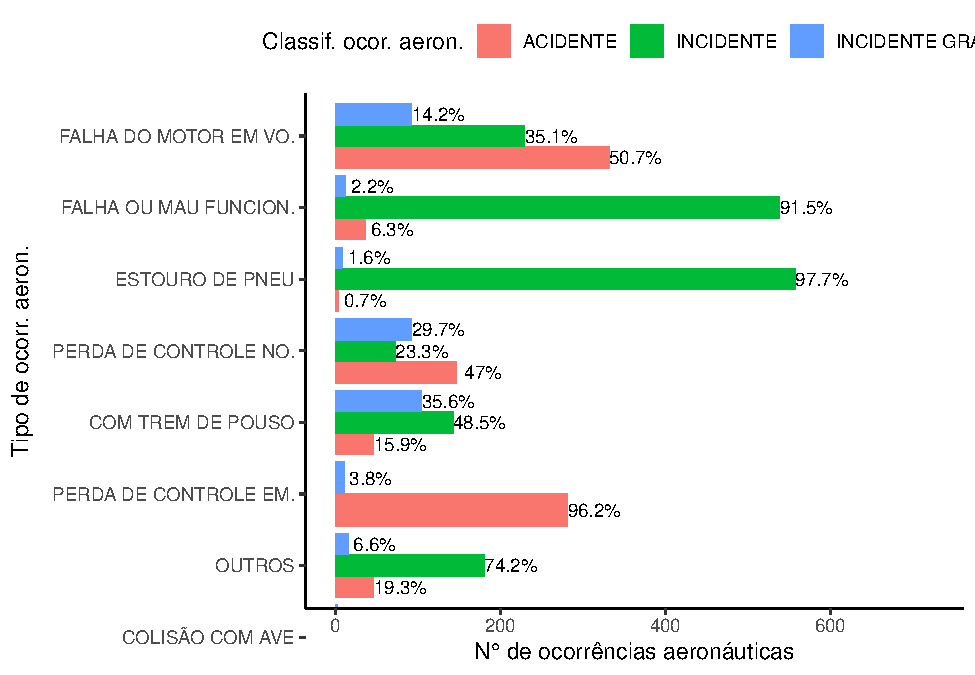
\includegraphics{4.Relatorio/pdf/index_files/figure-latex/unnamed-chunk-45-1} \end{center}

\begin{Shaded}
\begin{Highlighting}[]
\NormalTok{ggplot2\_ocor\_ocorrencia\_tipo\_new\_classif2 }\OtherTok{\textless{}{-}} \FunctionTok{grafico\_tab\_frequencia\_bivariada3}\NormalTok{(}
\NormalTok{    p\_ocor\_ocorrencia\_tipo\_new\_classif,}
    \StringTok{"ocorrencia\_classificacao"}\NormalTok{,}
    \StringTok{"ocorrencia\_tipo\_new"}\NormalTok{,}
    \AttributeTok{size =} \DecValTok{2}\NormalTok{,}
    \AttributeTok{tx1 =} \FloatTok{0.025}\NormalTok{,}
    \AttributeTok{tx2 =} \FloatTok{0.00025}\NormalTok{,}
    \AttributeTok{legend=}\ConstantTok{FALSE}
\NormalTok{) }\SpecialCharTok{+}\NormalTok{ gg}\SpecialCharTok{$}\FunctionTok{scale\_fill\_discrete}\NormalTok{(}\AttributeTok{name =} \StringTok{"Classif. ocor. aeron."}\NormalTok{) }\SpecialCharTok{+}
\NormalTok{    gg}\SpecialCharTok{$}\FunctionTok{theme}\NormalTok{(}\AttributeTok{legend.position=}\StringTok{"top"}\NormalTok{) }\SpecialCharTok{+} 
\NormalTok{    gg}\SpecialCharTok{$}\FunctionTok{coord\_flip}\NormalTok{(}\AttributeTok{xlim=}\FunctionTok{c}\NormalTok{(p\_ocor\_ocorrencia\_tipo\_new\_classif[[}\StringTok{\textquotesingle{}ocorrencia\_tipo\_new\textquotesingle{}}\NormalTok{]][}\DecValTok{1}\NormalTok{],}
\NormalTok{                         p\_ocor\_ocorrencia\_tipo\_new\_classif[[}\StringTok{\textquotesingle{}ocorrencia\_tipo\_new\textquotesingle{}}\NormalTok{]][}\DecValTok{20}\NormalTok{])) }\SpecialCharTok{+}
\NormalTok{    gg}\SpecialCharTok{$}\FunctionTok{scale\_x\_discrete}\NormalTok{(}
  \AttributeTok{labels =} \ControlFlowTok{function}\NormalTok{(x) \{}
\NormalTok{        is\_long }\OtherTok{\textless{}{-}} \FunctionTok{nchar}\NormalTok{(x) }\SpecialCharTok{\textgreater{}} \DecValTok{20}
\NormalTok{        x[is\_long] }\OtherTok{\textless{}{-}} \FunctionTok{paste0}\NormalTok{(}\FunctionTok{substr}\NormalTok{(x[is\_long], }\DecValTok{1}\NormalTok{, }\DecValTok{20}\NormalTok{), }\StringTok{"."}\NormalTok{)}
\NormalTok{        x}
\NormalTok{      \}) }\SpecialCharTok{+}
\NormalTok{    gg}\SpecialCharTok{$}\FunctionTok{ylab}\NormalTok{(}\StringTok{\textquotesingle{}Proporção de ocorrências aeronáuticas\textquotesingle{}}\NormalTok{) }\SpecialCharTok{+}
\NormalTok{    gg}\SpecialCharTok{$}\FunctionTok{xlab}\NormalTok{(}\StringTok{\textquotesingle{}Tipo de ocorr. aeron.\textquotesingle{}}\NormalTok{)}
\CommentTok{\# }
\end{Highlighting}
\end{Shaded}

\begin{Shaded}
\begin{Highlighting}[]
\NormalTok{p\_ocor\_ocorrencia\_tipo\_new\_classif3 }\OtherTok{\textless{}{-}}\NormalTok{ p\_ocor\_ocorrencia\_tipo\_new\_classif}
\NormalTok{aux }\OtherTok{\textless{}{-}}\NormalTok{ p\_ocor\_ocorrencia\_tipo\_new\_classif3 }\SpecialCharTok{\%\textgreater{}\%} 
\NormalTok{    dp}\SpecialCharTok{$}\FunctionTok{filter}\NormalTok{(}\StringTok{\textasciigrave{}}\AttributeTok{ocorrencia\_classificacao}\StringTok{\textasciigrave{}} \SpecialCharTok{==} \StringTok{"ACIDENTE"}\NormalTok{) }\SpecialCharTok{\%\textgreater{}\%} 
\NormalTok{    dp}\SpecialCharTok{$}\FunctionTok{arrange}\NormalTok{(dp}\SpecialCharTok{$}\FunctionTok{desc}\NormalTok{(}\StringTok{\textasciigrave{}}\AttributeTok{Percentage}\StringTok{\textasciigrave{}}\NormalTok{)) }\SpecialCharTok{\%\textgreater{}\%} 
\NormalTok{    dp}\SpecialCharTok{$}\FunctionTok{pull}\NormalTok{(ocorrencia\_tipo\_new)}
\NormalTok{p\_ocor\_ocorrencia\_tipo\_new\_classif3 }\OtherTok{\textless{}{-}}\NormalTok{ p\_ocor\_ocorrencia\_tipo\_new\_classif3 }\SpecialCharTok{\%\textgreater{}\%} 
\NormalTok{                    dplyr}\SpecialCharTok{::}\FunctionTok{arrange}\NormalTok{(}\FunctionTok{match}\NormalTok{(}\StringTok{\textasciigrave{}}\AttributeTok{ocorrencia\_tipo\_new}\StringTok{\textasciigrave{}}\NormalTok{, aux)) }\SpecialCharTok{\%\textgreater{}\%} 
\NormalTok{    dp}\SpecialCharTok{$}\FunctionTok{mutate}\NormalTok{(}\StringTok{\textasciigrave{}}\AttributeTok{ocorrencia\_tipo\_new}\StringTok{\textasciigrave{}} \OtherTok{=}\NormalTok{ bs}\SpecialCharTok{$}\FunctionTok{as.character}\NormalTok{(}\StringTok{\textasciigrave{}}\AttributeTok{ocorrencia\_tipo\_new}\StringTok{\textasciigrave{}}\NormalTok{)) }\SpecialCharTok{\%\textgreater{}\%} 
\NormalTok{    dp}\SpecialCharTok{$}\FunctionTok{mutate}\NormalTok{(}\StringTok{\textasciigrave{}}\AttributeTok{ocorrencia\_tipo\_new}\StringTok{\textasciigrave{}} \OtherTok{=}\NormalTok{ bs}\SpecialCharTok{$}\FunctionTok{ifelse}\NormalTok{(}\StringTok{\textasciigrave{}}\AttributeTok{ocorrencia\_tipo\_new}\StringTok{\textasciigrave{}} \SpecialCharTok{==} \StringTok{""}\NormalTok{, }\StringTok{"NULL"}\NormalTok{,}
                                             \StringTok{\textasciigrave{}}\AttributeTok{ocorrencia\_tipo\_new}\StringTok{\textasciigrave{}}\NormalTok{)) }\SpecialCharTok{\%\textgreater{}\%} 
\NormalTok{    dp}\SpecialCharTok{$}\FunctionTok{mutate}\NormalTok{(}\StringTok{\textasciigrave{}}\AttributeTok{ocorrencia\_tipo\_new}\StringTok{\textasciigrave{}} \OtherTok{=}\NormalTok{ fc}\SpecialCharTok{$}\FunctionTok{fct\_rev}\NormalTok{(fc}\SpecialCharTok{$}\FunctionTok{fct\_inorder}\NormalTok{(}\StringTok{\textasciigrave{}}\AttributeTok{ocorrencia\_tipo\_new}\StringTok{\textasciigrave{}}\NormalTok{)))}
    

\NormalTok{ggplot2\_ocor\_ocorrencia\_tipo\_new\_classif3 }\OtherTok{\textless{}{-}} \FunctionTok{grafico\_tab\_frequencia\_bivariada3}\NormalTok{(}
\NormalTok{    p\_ocor\_ocorrencia\_tipo\_new\_classif3,}
    \StringTok{"ocorrencia\_classificacao"}\NormalTok{,}
    \StringTok{"ocorrencia\_tipo\_new"}\NormalTok{,}
    \AttributeTok{size =} \FloatTok{1.8}\NormalTok{,}
    \AttributeTok{tx1 =} \FloatTok{0.025}\NormalTok{,}
    \AttributeTok{tx2 =} \FloatTok{0.00025}\NormalTok{,}
    \AttributeTok{legend=}\ConstantTok{FALSE}
    
\NormalTok{) }\SpecialCharTok{+}\NormalTok{ gg}\SpecialCharTok{$}\FunctionTok{scale\_x\_discrete}\NormalTok{(}
    \AttributeTok{labels =} \ControlFlowTok{function}\NormalTok{(k) \{}
\NormalTok{        is\_long }\OtherTok{\textless{}{-}} \FunctionTok{nchar}\NormalTok{(k) }\SpecialCharTok{\textgreater{}} \DecValTok{19}
\NormalTok{        k[is\_long] }\OtherTok{\textless{}{-}} \FunctionTok{paste0}\NormalTok{(}\FunctionTok{substr}\NormalTok{(k[is\_long], }\DecValTok{1}\NormalTok{, }\DecValTok{19}\NormalTok{), }\StringTok{"."}\NormalTok{)}
\NormalTok{        k}
\NormalTok{    \}}
\NormalTok{) }\SpecialCharTok{+}
\NormalTok{    gg}\SpecialCharTok{$}\FunctionTok{coord\_flip}\NormalTok{(}
        \AttributeTok{xlim =} \FunctionTok{c}\NormalTok{(}
\NormalTok{            p\_ocor\_ocorrencia\_tipo\_new\_classif3[[}\StringTok{\textquotesingle{}ocorrencia\_tipo\_new\textquotesingle{}}\NormalTok{]][}\DecValTok{1}\NormalTok{],}
\NormalTok{            p\_ocor\_ocorrencia\_tipo\_new\_classif3[[}\StringTok{\textquotesingle{}ocorrencia\_tipo\_new\textquotesingle{}}\NormalTok{]][}\DecValTok{30}\NormalTok{]}
\NormalTok{        )}
\NormalTok{    ) }\SpecialCharTok{+}
\NormalTok{    gg}\SpecialCharTok{$}\FunctionTok{scale\_fill\_discrete}\NormalTok{(}\AttributeTok{name =} \StringTok{"Classif. ocor. aeron."}\NormalTok{) }\SpecialCharTok{+}
\NormalTok{    gg}\SpecialCharTok{$}\FunctionTok{theme}\NormalTok{(}\AttributeTok{legend.position =} \StringTok{"top"}\NormalTok{) }\SpecialCharTok{+}
\NormalTok{    gg}\SpecialCharTok{$}\FunctionTok{ylab}\NormalTok{(}\StringTok{\textquotesingle{}Proporção de ocorrências aeronáuticas\textquotesingle{}}\NormalTok{) }\SpecialCharTok{+}
\NormalTok{    gg}\SpecialCharTok{$}\FunctionTok{xlab}\NormalTok{(}\StringTok{\textquotesingle{}Tipo de ocorr. aeron.\textquotesingle{}}\NormalTok{)}
\end{Highlighting}
\end{Shaded}

\begin{Shaded}
\begin{Highlighting}[]
\DocumentationTok{\#\#\#\#\#\#\#\#\#\#\#\#\#\#\#\#\#\#\#\#\#\#\#\#\#\#\#\#\#\#\#\#\#\#\#\#\#\#\#\#\#\#\#\#\#\#\#\#\#\#\#\#\#\#\#\#\#\#\#\#\#\#\#\#\#\#\#\# Salva gráfico}

\CommentTok{\#source(\textquotesingle{}funcoes\_auxiliares/salva\_grafico.R\textquotesingle{}, encoding = "UTF{-}8")}
\FunctionTok{salva\_grafico}\NormalTok{(}\AttributeTok{ggplot2\_grafico =}\NormalTok{ ggplot2\_ocor\_ocorrencia\_tipo\_new\_classif2, }\AttributeTok{y=}\FloatTok{1.14}\NormalTok{)}

\DocumentationTok{\#\#\#\#\#\#\#\#\#\#\#\#\#\#\#\#\#\#\#\#\#\#\#\#\#\#\#\#\#\#\#\#\#\#\#\#\#\#\#\#\#\#\#\#\#\#\#\#\#\#\#\#\#\#\#\#\#\#\#\#\#\#\#\#\#\#\#\# Leitura gráfico}

\CommentTok{\#source(\textquotesingle{}funcoes\_auxiliares/leitura\_grafico.R\textquotesingle{}, encoding = "UTF{-}8")}
\FunctionTok{leitura\_grafico}\NormalTok{(}\AttributeTok{ggplot2\_grafico =}\NormalTok{ ggplot2\_ocor\_ocorrencia\_tipo\_new\_classif2)}
\end{Highlighting}
\end{Shaded}

\begin{center}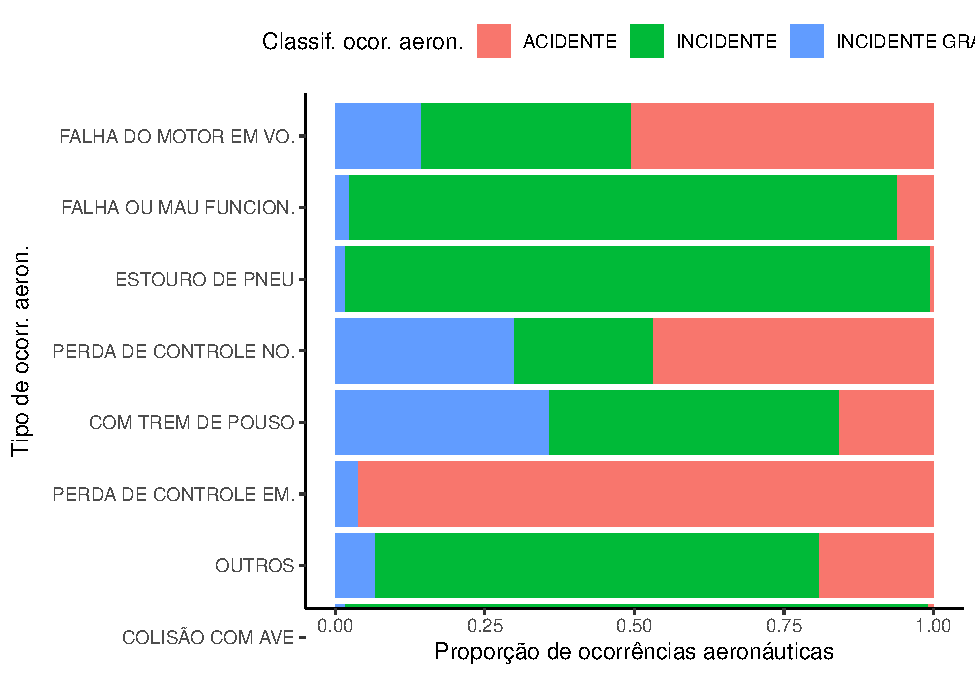
\includegraphics{4.Relatorio/pdf/index_files/figure-latex/unnamed-chunk-48-1} \end{center}

\begin{Shaded}
\begin{Highlighting}[]
\DocumentationTok{\#\#\#\#\#\#\#\#\#\#\#\#\#\#\#\#\#\#\#\#\#\#\#\#\#\#\#\#\#\#\#\#\#\#\#\#\#\#\#\#\#\#\#\#\#\#\#\#\#\#\#\#\#\#\#\#\#\#\#\#\#\#\#\#\#\#\#\# Salva gráfico}

\CommentTok{\#source(\textquotesingle{}funcoes\_auxiliares/salva\_grafico.R\textquotesingle{}, encoding = "UTF{-}8")}
\FunctionTok{salva\_grafico}\NormalTok{(}\AttributeTok{ggplot2\_grafico =}\NormalTok{ ggplot2\_ocor\_ocorrencia\_tipo\_new\_classif3, }\AttributeTok{y=}\FloatTok{1.14}\NormalTok{)}

\DocumentationTok{\#\#\#\#\#\#\#\#\#\#\#\#\#\#\#\#\#\#\#\#\#\#\#\#\#\#\#\#\#\#\#\#\#\#\#\#\#\#\#\#\#\#\#\#\#\#\#\#\#\#\#\#\#\#\#\#\#\#\#\#\#\#\#\#\#\#\#\# Leitura gráfico}

\CommentTok{\#source(\textquotesingle{}funcoes\_auxiliares/leitura\_grafico.R\textquotesingle{}, encoding = "UTF{-}8")}
\FunctionTok{leitura\_grafico}\NormalTok{(}\AttributeTok{ggplot2\_grafico =}\NormalTok{ ggplot2\_ocor\_ocorrencia\_tipo\_new\_classif3)}
\end{Highlighting}
\end{Shaded}

\begin{center}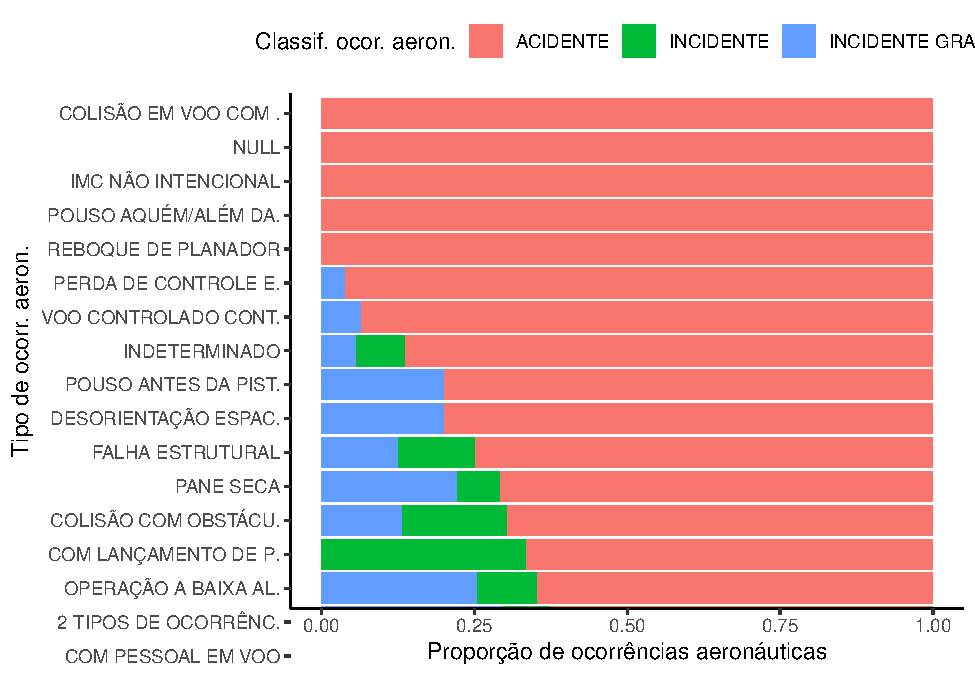
\includegraphics{4.Relatorio/pdf/index_files/figure-latex/unnamed-chunk-48-2} \end{center}

\begin{quote}
É possível observar que existem vários tipos de ocorrência, porém alguns
tipos são mais propensos a serem classificados como acidentes, tais
como: Perda de controle em voo, pane seca, operação a baixa altitude,
etc.
\end{quote}

\hypertarget{conclusuxf5es-e-insights-gerados}{%
\section{Conclusões e insights
gerados}\label{conclusuxf5es-e-insights-gerados}}

\begin{quote}
Apesar de incidentes (\textasciitilde{} 54.4\%) ocorrerem mais do que
incidentes graves ou acidentes (\textasciitilde{} 45.6\%), este último
número ainda é preocupante. O ideal é que se tenha uma porcentagem mais
baixa de incidentes graves e acidentes para que pessoas não sofram
qualquer lesão corporal.
\end{quote}

\begin{quote}
É possível perceber que o número absoluto de ocorrências aeronáuticas
teve uma queda até o ano de 2016 e voltou a subir a partir desse ano.
Nota-se que essa tendência também ocorre nas ocorrências de
classificação do tipo ``INCIDENTE'' e em menor grau na classificação do
tipo ``INCIDENTE GRAVE''. Comportamento diferente é observado na
tendência do número de ocorrências aeronáuticas com classificação do
tipo ``ACIDENTE'' que se manteve em queda desde 2012. Além disso, é
importante ressaltar que as somas das frequências relativas de
``ACIDENTES'' e ``INCIDENTES GRAVES'' ao longo dos anos variaram com
valores mínimo e máximo iguais à 41\% em 2013 e 55.2\% em 2018,
respectivamente.
\end{quote}

\begin{quote}
Naturalmente, pelo fato de existir maior movimentação de aviões em
estados de alta atividade econômica, esses mesmos têm as maiores
quantidades de ocorrências. Porém, são os estados de
MT(\textasciitilde56.9\%), RR(\textasciitilde55.6\%), e
SE(\textasciitilde50\%) que têm as maiores proporções de acidentes.
\end{quote}

\begin{quote}
Não se observa uma quantidade maior de ocorrências nas saídas de pista,
porém a proporção de ocorrências classificadas como acidentes é maior
quando se tem uma ocorrência na saída de pista (51.8\% \textgreater{}
30.3\%).
\end{quote}

\begin{quote}
É possível observar que existem vários tipos de ocorrência, porém alguns
tipos são mais propensos a serem classificados como acidentes, tais
como: Perda de controle em voo, pane seca, operação a baixa altitude,
etc.
\end{quote}

\hypertarget{referuxeancias}{%
\section{Referências}\label{referuxeancias}}

\begin{itemize}
\tightlist
\item
  \href{https://www3.fmb.unesp.br/sete/pluginfile.php/20354/mod_page/content/2/A_Investigacao_de_acidentes_aeronauticos_Conforme_a_Lei_no_7.pdf}{A
  Investigação de acidentes aeronáuticos}
\item
  \href{https://dados.gov.br/dataset/ocorrencias-aeronauticas-da-aviacao-civil-brasileira}{CENIPA
  - Ocorrências Aeronáuticas na Aviação Civil Brasileira}
\item
  \href{https://www.tidyverse.org/}{tidyverse}
\item
  \href{https://dplyr.tidyverse.org/}{dplyr}
\item
  \href{https://ggplot2.tidyverse.org/}{ggplot2}
\item
  \href{https://dbi.r-dbi.org/}{DBI}
\item
  \href{https://rpostgres.r-dbi.org/}{RPostgres}
\item
  \href{http://www.htmlwidgets.org/index.html}{htmlwidgets}
\item
  \href{https://plot.ly/r}{Plotly}
\item
  \href{https://www.highcharts.com/}{HighCharts}
\item
  \href{http://jkunst.com/highcharter/}{HighCharter}
\item
  \href{https://www.tmbish.me/lab/highcharter-cookbook/}{HighCharter
  Cookbook - Tom Bishop}
\item
  \href{https://rmarkdown.rstudio.com}{R Markdown}
\item
  \href{http://yihui.name/knitr}{knitr}
\item
  \href{https://github.com/yihui/xaringan}{yihui/xaringan}
\item
  \href{https://github.com/gadenbuie/xaringanthemer}{gadenbuie/xaringanthemer}
\item
  \href{https://github.com/gadenbuie/xaringanExtra}{gadenbuie/xaringanExtra}
\item
  \href{https://r-ladies-sao-paulo.github.io/xaringan/slides.html\#7}{Imagem:
  Ilustração por Allison Horst - Twitter: @allison\_horst - Adaptado de
  Wickham e Grolemund, 2017}
\item
  \href{https://hbctraining.github.io/In-depth-NGS-Data-Analysis-Course/sessionVI/lessons/knitr_rmarkdown.html}{Imagem:
  Reproducible reports in R}
\end{itemize}

\end{document}
